\documentclass[
    a4paper,
    brazil,
    12pt,
        ]{icmc}

%\voffset=0pt
%\usepackage[none]{hyphenat}	para evitar hifenizacao
\hyphenpenalty=2000 		% (nao ta funcionando)
\tolerance=400			%
\clubpenalty=10000		% Altera��o Vin�cius
\widowpenalty=10000		%
\displaywidowpenalty=10000	%

% alteracao Vin�cius
%\usepackage{tocloft}

%\newlength\mylena
%\settowidth\mylena{Figura}
%\newlength\mylenb
%\settowidth\mylenb{Tabela}

%\addtolength\cftfignumwidth{\mylena}
%\addtolength\cfttabnumwidth{\mylenb}

%\renewcommand\cftfigpresnum{Figura }
%\renewcommand\cfttabpresnum{Tabela }
%fim
%
\usepackage{listings,listings}

\usepackage{pdfpages}
\usepackage[brazil]{babel}
\usepackage[latin1]{inputenc}

%Landir -------------------------------------------
\usepackage{multirow}
\newcommand{\conj}[4]{#1=\{#3~|~#2 \leq #3 \leq #4, ~#3 \in \mathbb{N}\}}
\newcommand{\matrizz}[7]{#1_{#2 \times #3} \textrm{, } #4_{#5 #6} \in \mathbb{#7}}
\newcommand{\matrizzz}[9]{#1_{#2 \times #3 \times #4} \textrm{, } #5_{#6 #7 #8} \in \mathbb{#9}}
\newcommand{\interval}[3]{#1 \leq #2 \leq #3}
\newcommand{\quintupla}[5]{\langle #1,#2,#3,#4,#5 \rangle}
\newcommand{\tripla}[3]{\langle #1,#2,#3 \rangle}
\newcommand{\parord}[2]{\langle #1,#2 \rangle}

%ambiente para defini��es, teoremas etc...
\newtheorem{defi}{Defini��o}[chapter]
\newtheorem{propri}{Propriedade}[chapter]
\newtheorem{conce}{Conceito}[chapter]
\newtheorem{propo}{Proposi��o}[chapter]
\newcommand{\dsum}{\displaystyle\sum}
\usepackage{algorithm}
\usepackage{clrscode3e}
\usepackage{lscape}	%pagina em formato paisagem
%--------------------------------------------------

\usepackage[toc,page]{appendix}
\usepackage{isoaccent}
\usepackage{setspace}
\usepackage{babel}
\usepackage{float}
\usepackage{longtable}
\usepackage[nottoc]{tocbibind}
\usepackage{graphicx}
\usepackage{epstopdf}
%--------------------------------------------------
\usepackage{subfigure}
\graphicspath{{figuras/}}

%--------------------------------------------------

\usepackage{amssymb, amsmath}
%% --------------------------------------------------------------
%% se for quali, substitua "capaUEM" por "capaUEMquali" 
\usepackage{capaUEM}      % Para formata��o de capa e folhas de rosto
%%
%% ---------------------------------------------------------------
\usepackage[
    sort&compress,
    %numbers,
    authoryear,
    ]{natbib} % Para usar estilo novo de refer�ncias
\usepackage{verbatim}
\usepackage{titlesec}
\usepackage{enumerate}
\usepackage{pdfpages}
\usepackage{colortbl}
\usepackage{color}
\usepackage{textfit}
\usepackage{tabularx}
\usepackage{rotating}
\usepackage{fancyhdr}
\usepackage{url}
\usepackage{placeins}
\usepackage{afterpage}
\usepackage{setspace}
\usepackage{amsmath}

\usepackage{booktabs}
\usepackage{adjustbox}

%\singlespacing
\onehalfspacing
%\doublespacing
%\setstretch{1.1}

\RequirePackage{ifthen}
%
% Importando APUD do abntcite.sty
%
\newcommand{\apudname}{apud}
\def\citeopen{(}
\def\citeclose{)}

\newcommand{\apud}[3][]{\citeopen\citeauthor{#2}, \citeyear{#2} \apudname\ %
\citeauthor{#3}, \citeyear{#3}%
\ifthenelse{\equal{#1}{\empty}}{}{, #1}\citeclose}

\let\cite=\citep    % O natbib requer \citep para refer�ncias. Ent�o, se vc j� escreveu muita coisa usando \cite, este comando substitui na hora de compilar

\usepackage[a4paper, top=3cm, bottom=2cm, %   footskip=15pt,
    verbose,
    left=3cm,
    right=2cm,
  ]{geometry}

%\widowpenalty=350 % comentado por Vinicius
%\clubpenalty=350  % ''

\exhyphenpenalty=10000 \hyphenpenalty=800

\vfuzz1pc % Don't bother to report overfull boxes if over-edge is < 1pc
\hfuzz1pc % Don't bother to report overfull boxes if over-edge is < 1pc

\newcommand{\atributo}[1]{\textbf{\textit{#1}}}


%% Limpa os cabe�alhos, deixando s� o n�mero da p�gina
\renewcommand{\headrulewidth}{0pt}
\pagestyle{fancyplain}
\fancyhf{}
\rhead{\fancyplain{}{\thepage}}

%% Muda a formata�ao dos t�tulos das listas de figuras, tabelas e sum�rio
\makeatletter

\def\tableofcontents{
\newpage
\pagestyle{empty}
\centerline{\large \textbf{SUM�RIO}}
\@mkboth{SUM�RIO}{SUM�RIO}
\@starttoc{toc}
}

\def\listoffigures{
\newpage
\pagestyle{empty}
\centerline{\large LISTA DE FIGURAS}
\@mkboth{LISTA DE FIGURAS}{LISTA DE FIGURAS}
\@starttoc{lof}
}



\def\listoftables{
\newpage
\pagestyle{empty}
\centerline{\large LISTA DE TABELAS}
\@mkboth{LISTA DE TABELAS}{LISTA DE TABELAS}
\@starttoc{lot}
}
\makeatother
\hyphenation{proba-bi-li-da-des}
\hyphenation{apre-sen-tar}
\hyphenation{gra-ma-ti-cais}
\hyphenation{e-qui-va-le}
\hyphenation{es-ta-be-le-ci-das}
\hyphenation{cate-goria}

%%%%%%%%%%%%%%%%%%%%%%%%%%%%%%%%%%%%%%%%%%%%%%%%%%%%%%%%%%%%%%%%%%%%%%%%%%%%%%%%%%%%%%%%%%%%%%%%%%%
% Estilos diferentes para cabe�alho de cap�tulo - by Adenilso
%%%%%%%%%%%%%%%%%%%%%%%%%%%%%%%%%%%%%%%%%%%%%%%%%%%%%%%%%%%%%%%%%%%%%%%%%%%%%%%%%%%%%%%%%%%%%%%%%%%

\makeatletter  %usado para que o @ seja considerado
 \newcounter{capkind}
 \setcounter{capkind}{1}   % define qual tipo de cabe�alho usar
    
     
 \ifcase\value{capkind}
 \def\@makechapterhead#1{%
 \begingroup
 \centering
   \vspace*{50\p@}%
         \noindent\begin{tabular}{p{0.34\textwidth}|p{0.22\textwidth}|p{0.34\textwidth}}
   \cline{2-2}
   \raisebox{0pt}[25pt][15pt]{}& \centering\large{\sffamily\scshape{\@chapapp}}\space \itshape\thechapter & \\
   \hline
   \hline
       \multicolumn{3}{|p{0.97\textwidth}|}{\raisebox{0pt}[30pt][20pt]{}\centering\Huge \bfseries #1}\\
   \hline
   \hline
   \raisebox{0pt}[10pt][10pt]{}&  & \\	
   \cline{2-2}
   \end{tabular}\par
   \vspace*{40\p@}%
 \endgroup
 }
 \def\@makeschapterhead#1{%
 \begingroup
 \centering
   \vspace*{50\p@}%
         \noindent\begin{tabular}{p{0.34\textwidth}|p{0.22\textwidth}|p{0.34\textwidth}}
   \cline{2-2}
   \raisebox{0pt}[10pt][10pt]{}&  & \\
   \hline
   \hline
       \multicolumn{3}{|p{0.97\textwidth}|}{\raisebox{0pt}[30pt][20pt]{}\centering\Huge \bfseries #1}\\
   \hline
   \hline
   \raisebox{0pt}[10pt][10pt]{}&  & \\	
   \cline{2-2}
   \end{tabular}\par
   \vspace*{40\p@}%
 \endgroup
 }
 \or %%%%%%%%%%%%%%%%%%%%%%%
 
 \def\@makechapterhead#1{%
 \begingroup
   \vspace*{50\p@}%
      \noindent
       \sffamily\Huge\hrulefill          
      {\begin{tabular}{|c|}
          %\rowcolor{black}
          \hline
          \color{white} \large \scshape % \@chapapp{} \\
          %\hline
          \vspace{-2ex}\\ %coloquei para aumentar o espa�o entre o t�tulo e o n�mero
          \Huge \slshape \scaletoheight{1cm}{\thechapter} \\ \hline
      \end{tabular}     
      }
   
      \par
      \vspace*{18\p@}
      {\Huge\bfseries\begin{flushright} #1\end{flushright}}\par
      \vspace*{-6\p@}
      \hspace*{0pt plus 1fill}
     	\rule{.8\textwidth}{0.5pt}\\[-36\p@]
     \hspace*{0pt plus 1fill}
      \rule{.8\textwidth}{3pt}
      \vskip 1.7ex
 \endgroup
     }
                               
 \def\@makeschapterhead#1{%       Essa parte configura o cabe�alho do cap�tulo refer�ncias
  
 \begingroup
   \vspace*{30\p@}%
      \noindent
      \sffamily\Huge
      {\Huge\bfseries \begin{flushright} #1\end{flushright}}\par
      \vspace*{0\p@}
 %     \hspace*{0pt plus 1fill}
 %     	\rule{.8\textwidth}{0.5pt}\par
      \vspace*{-12\p@}
      \hspace*{0pt plus 1fill}
       \rule{.8\textwidth}{3pt}
      \vskip 1.7ex
      
 \endgroup
      
   
     }
     \def\@schap#1{%      
  	 \begingroup
   \vspace*{30\p@}%
      \noindent
      \sffamily\Huge
      {\Huge\bfseries \begin{flushright} #1\end{flushright}}\par
      \vspace*{0\p@}
 %     \hspace*{0pt plus 1fill}
 %     	\rule{.8\textwidth}{0.5pt}\par
      \vspace*{-12\p@}
      \hspace*{0pt plus 1fill}
       \rule{.8\textwidth}{3pt}
      \vskip 1.7ex
      
 \endgroup
      
   
     }

  


\fi

\makeatother %para voltar a ignorar o @
%\includeonly{gerenciamento}
\begin{document}

%%%%%%%%%%%%%%%%%%%%%%%%%%%%%%%%%%%%%%%%%%%%%%%%%%%%%%%%%%%%%%%%%%%%%%%%%%%%%%%%%%%%%%%%%%%%%%%%%%%
%% DADOS PARA CAPA, FOLHA DE ROSTO E FOLHA DE APROVAO

% Dados autor
\Jautor{HENRIQUE VIGNANDO}

% Dados trabalho: ttulo e subttulo (opcional)

\Jtitulo{Uma Ontologia para Experimentos e Quasi-Experimentos Controlados para Linha de Produto de Software - OntoExper-LPS}
%\Jsubtitulo{: uma nova soluo ...} %% descomente essa linha caso haja um subttulo
%\Jtituloabs{Efficient neighborhood ... applied to the ...}
%\Jsubtituloabs{: a new solution...} %% descomente essa linha caso haja um subttulo

% Ano da defesa
\Jdata{2020}

% Dados orienta��o
\Jtipoorientador{o} %% caso seja orientador
\Jorientador{Edson A. Oliveira Junior}
%\JtipobancaC{o} %% caso seja professor (usado na folha de aprovao)

%\Jcoorientador{o}{Edson Oliveira Junior} %% caso no haja coorientador(a) comente esta linha e a prxima
%\Jtipocoorientador{o} %% caso seja coorientador
%\Jtipocoorientador{a} %% caso seja coorientadora
%\JtipobancaC{a}  %% caso seja professora (usado na folha de aprovao)


% Dados da banca
%\JtipobancaA{a} %% caso seja professora
\JtipobancaA{o}  %% caso seja professor
\JbancaA{Fulano 1}
\JinstituicaoA{Universidade Estadual de Maring� --- DIN/UEM}

%\JtipobancaB{a}  %% caso seja professora
\JtipobancaB{o} %% caso seja professor
\JbancaB{Fulano 2}
\JinstituicaoB{Universidade Federal do Fim do Mundo --- DEINFO/UFFM}

% Dados da defesa
\Jdatadefesa{21 de Fevereiro de 2019.}
\Jlocaldefesa{Sala 101, Bloco C56, \textit{campus} da Universidade Estadual de Maring�.}


%%%%%%%%%%%%%%%%%%%%%%%%%%%%%%%%%%%%%%%%%%%%%%%%%%%%%%%%%%%%%%%%%%%%%%%%%%%%%%%%%%%%%%%%%%%%%%%%%%%
\frontmatter
\Jcapa
\mainmatter

\Jfolhaderosto


%\Jfichacatalografica
%\include{ficha}
%\include{errata}
\Jfolhaaprovacao
\geometry{left=2.5cm}


\geometry{left=3cm}
%\include{dedicatoria}
\clearpage
\thispagestyle{empty}

\begin{center}	
	{\large AGRADECIMENTOS}
\end{center}
%\vspace*{0.5cm}
\normalsize
\noindent


Agrade�o a Deus por ter me aben�oado nesta caminhada e as pessoas que contribu�ram na realiza��o deste trabalho. Em especial:

A minha fam�lia pelo carinho, apoio e incentivo.

Ao meu orientador professor Dr. xxxxxxxxxxxx pelo apoio, coment�rios e sugest�es no desenvolvimento deste projeto.

Aos demais professores das disciplinas que cursei e aos colegas ...

E a Coordena��o de Aperfei�oamento de Pessoal de N�vel Superior (CAPES) pelo apoio financeiro concedido a este trabalho.


\clearpage
\thispagestyle{empty}

\noindent{\large\bf\dadoTitulo}
\noindent{\large\dadoSubTitulo}

\normalsize
\begin{center}	
	\vspace*{0.5cm}
	\textbf{RESUMO}
\end{center}

O processo de experimentação em Engenharia de Software (ES) é fundamental para ciclo de vida de um software. Com ele é possível reduzir grandes esforços de desenvolvimento e principalmente de manutenção. A comunidade de ES vem discutindo e avaliando como melhorar a qualidade dos experimentos, visando aumentar a confiabilidade dos seus resultados. Por mais que eles tem abordado a qualidade de experimentos controlados de forma geral, ainda não há evidencias que estão analisando em contextos específicos, como é o caso de Linhas de produto de Software (LPS). Neste caso, ainda existe uma falta de instrumentação e medição especifica da qualidade dos experimentos em LPS. Por isso torna-se necessário fornecer um corpo de conhecimento confiável e replicável no contexto de LPS. Devido essa importância, projetar, executar e analisar os resultados de um experimento em LPS torna-se crucial para garantir a qualidade dos mesmos. Neste sentido propomos uma ontologia (SMartyOntology) para experimentos em LPS, pois possui centenas de experimentos publicados. A ontologia é concebida principalmente com base em diretrizes definidas e é projetada usando linguagem OWL, suportada pelo ambiente Protégé para verificação de sintaxe e avaliação inicial. A ontologia foi preenchida com mais de 150 experimentos em linhas de produtos de software, reunidos em um estudo de mapeamento sistemático. Surge também a oportunidade de investigar a elaboração de um sistema de recomendação para experimentos em LPS se baseando em na modelagem de informação estruturada pela ontologia proposta. Portanto, este trabalho apresenta conceitos fundamentais para elaboração de uma ontologia voltada para experimentos em LPS, e para criação de um sistema de recomendação para experimentos em LPS. Acreditamos que essa ontologia  bem como o sistema de recomendação pode contribuir para documentar melhor os elementos essenciais de um experimento, promovendo assim a repetição, a replicação e a reprodutibilidade dos experimentos. Na qual, possa levar qualidade para os projetos experimentais e resultados obtidos por meio dos experimento recomendados. Ontologias e Sistemas de recomendação são bem conhecidos na ES, acredita-se ser possível aplicar essas teorias para recomendar experimentos em LPS. Apresentamos também uma avaliação de viabilidade da ontologia proposta. Ao final temos um sistema de recomendação que apresenta bons resultados em recomendações para experimentos controlado. Espera-se também com este projeto, contribuir com a comunidade de LPS no sentido de melhorar os projetos e execução de experimentos, aumentando a confiança do corpo de conhecimento visando a transferência de tecnologia para indústria.\\

\noindent \textbf{Palavras-chave:} Experimento Controlado de Software. Linha de Produto de Software. Ontologia. Qualidade de Experimentos. Sistemas de Recomendação em Engenharia de Software. Sistemas de Recomendação.

\pagebreak

\clearpage
\thispagestyle{empty}

\noindent{\large\bf\dadoTituloAbs}
\noindent{\large\dadoSubTituloAbs}

\normalsize
\begin{center}	
	\vspace*{0.5cm}
	\textbf{\textit{ABSTRACT}}
\end{center}

The process of experimentation in Software Engineering (ES) has been fundamental for the software life cycle. With it it is possible to reduce major development efforts and especially maintenance. The higher education community has been discussing and evaluating how to improve the quality of higher education experiments in order to increase the reliability of their results. As much as the quality of experiments has been addressed, there is still a lack in specific contexts, such as Software Product Lines (LPS). Thus, planning, executing, and analyzing the results of an LPS experiment becomes crucial in supporting the evolution of LPS and providing a reliable and auditable body of knowledge. In this sense, this paper presents an ontology to support LPS experiments, OntoExper-SPL. The ontology was designed based on predefined guidelines, designed using the Ontology Web Language (OWL) text and supported by the Prot�g� environment. OntoExper-SPL was populated with over 200 LPS experiments. The ontology was evaluated based on a feasibility study with 17 LPS and ontology specialists. In addition, a Prototype Recommendation System (SR) capable of using ontology to make inferences about data from LPS experiments was implemented. Thus, it is believed that ontology can directly contribute to better documentation of LPS experiments, disseminate LPS experimentation knowledge, support the culture of experimentation in academia and industry, and improve software design and experiment execution by increasing the confidence of the body of knowledge to transfer technology to industry. \\

\noindent \textbf{\textit{Keywords:}} Experiment in SPL. Software Product Line. Ontology. Ontology in Software Engineering. Software Engineering Recommendation System. Recommendation Systems.

\pagebreak

 


\listoffigures

\listoftables

\clearpage
\thispagestyle{empty}

\noindent{\large\bf\dadoTituloAbs}
\noindent{\large\dadoSubTituloAbs}

\normalsize
\begin{center}
	LISTA DE SIGLAS E ABREVIATURAS
\end{center}


\noindent{\textbf{ALM}}: \textit{Application Lifecycle Management}

\noindent{\textbf{API}}: \textit{Application Programming Interface}

\noindent{\textbf{AQ}}: Avaliação de Qualidade

\noindent{\textbf{CBF}}: \textit{Content-based Filterin}

\noindent{\textbf{ES}}: Engenharia de Software

\noindent{\textbf{ETL}}: \textit{Extract, Transform, Load}

\noindent{\textbf{GRSSE}}: Grupo de pesquisa em Reuso Sistemático de Software e Experimentação

\noindent{\textbf{ID}}: Identificador Único

\noindent{\textbf{LPS}}: Linha de Produto de Software

\noindent{\textbf{PDI}}: \textit{Pentaho Data Integration}

\noindent{\textbf{POO}}: Programação Orientado a Objetos

\noindent{\textbf{RSSE}}: \textit{Recommendation System in Software Engineering}


\pagebreak
\tableofcontents

\chapter{Introdu��o}
\pagestyle{plain}

\section{Contextualiza��o}

Experimenta��o em Engenharia de Software (ES) tem se tornado fundamental para desenvolver e melhorar m�todos e ferramentas, bem como melhorar os processos de manuten��o de software \cite{kitchenham2007large}. Essa discuss�o permite que o conhecimento seja gerado de forma sistem�tica, disciplinada, quantific�vel e controlada \cite{wohlin2012experimentation}. Dessa forma, melhorando-se a qualidade dos experimentos \footnote[1]{Neste trabalho usaremos o termo "experimento" para denotar ambos os conceitos de ``experimento'' e ``\textit{quasi}-experimento''.} pode ser obtido um corpo de conhecimento confi�vel e referente em um dado t�pico de pesquisa. 

Atualmente, n�o h� diretrizes espec�ficas para avaliar a qualidade de experimentos em ES especialmente. Para �reas emergentes e em processo de consolida��o como � o caso de Linha de Produto de Software (LPS), em que aspectos espec�ficos do dom�nio como, por exemplo, os artefatos utilizados como objetos experimentais, a complexidade do treinamento, a dificuldade de sele��o de participantes qualificados e a falta de reposit�rios, podem influenciar os experimentos. Al�m disso, tem-se percebido uma constante car�ncia de documenta��o adequada dos experimentos que acabam por inviabilizar a repeti��o e auditoria dos estudos em LPS \cite{Furtado2018}.

Para permitir a repeti��o, reprodu��o e a replica��o de experimento � necess�ria uma formaliza��o dos principais conceitos. Para isso, pode-se obter vantagem do uso de ontologias.

Ontologias est�o entre os m�todos mais utilizados para formalizar informa��es. Ontologias s�o representa��es formais de uma abstra��o contendo defini��es formais de nomenclatura, conceitos, propriedades e rela��es entre os conceitos, a fim de definir um vocabul�rio controlado de termos e rela��es de conceitos \cite{gruber1993ontology}. Assim, o uso de ontologias para representar informa��es sobre experimentos permite padronizar dados facilitando a interoperabilidade, a troca de informa��es e a replica��o de experimentos.

Por mais atraente que seja, uma solu��o geral de ontologia para experimentos de ES � muito esparsa. Dadas as particularidades de cada t�pico de pesquisa em ES, seria complexo projetar uma ontologia capaz de representar todas as caracter�sticas particulares de cada t�pico. Dessa forma este trabalho, concentra esfor�os no campo de LPS, por causa da ampla gama de dados de experimentos neste assunto e experi�ncia do grupo de pesquisa em experimenta��o de LPS da UEM \cite{Furtado2018}.

% devido � nossa experi�ncia em grupo, uma vez que um mapeamento sistem�tico foi realizado em centenas de experimentos publicados em LPS \cite{Furtado2018}. (Grupo de Pesquisa em Reutiliza��o Sistem�tica de Software e Experimenta��o Cont�nua - GReater).

% Uma LPS � determinado por um conjunto e produtos de um determinado segmento de mercado (Northrop et al., 2007), como um sistema para aparelhos celulares, onde h� ativos centrais com as principais funcionalidades que o software deve implementar, chamadas semelhan�as, e pode haver um conjunto de funcionalidades espec�ficas para determinados dispositivos, chamados variabilidades. 

Experimentos no campo de LPS requerem consider�vel experi�ncia em ES, pois durante o planejamento e execu��o dos experimentos v�rios artefatos espec�ficos de ES e LPS podem ser gerados. Assim, a curva de aprendizado � longa o suficiente para extrair e apresentar os resultados de experimentos de LPS satisfatoriamente \cite{Furtado2018} e \cite{Furtado2019JCR}.

Portanto, a defini��o de uma ontologia para experimentos de LPS se destina a apoiar pesquisadores e profissionais no desenvolvimento e replica��o de experimentos, al�m de auxiliar na auditoria e valida��o de experimentos baseados em diretrizes determinadas pela ontologia.

Al�m disso, dados formalmente representados permitem o desenvolvimento de sistemas especialistas, como sistemas de recomenda��o. Um sistema de recomenda��o para experimenta��o ES poderia ser �til de duas maneiras: (i) didaticamente, para ajudar alunos, professores e profissionais a pesquisar experimentos relacionados; e, (ii) ajudar os profissionais da Engenharia de Software Experimental (ESE) a planejar e executar um experimento seguindo a experi�ncia de outros, baseando-se em consultas e recomenda��es de experimentos correlacionadas � sua �rea de atua��o.

% Portanto, o objetivo deste trabalho de mestrado � propor uma ontologia para representar formalmente essa diretriz, a fim de padronizar os experimentos de SPL. Esperamos facilitar a representa��o dos dados de experimentos para aumentar o uso geral de experimenta��o em ES, aumentar o n�mero de replica��es e o compartilhamento de dados.

% Resultados obtidos com a avalia��o da qualidade e viabilidade da ontologia indicam a possibilidade de criar infer�ncias aos dados e diretrizes sobre os experimentos, dessa forma � poss�vel criar como prova de conceito, modelos de infer�ncia para um sistema de recomenda��o sobre esta proposta de ontologia.


\section{Motiva��o e Justificativa}
\label{sec:motivacao}

Realizar um experimento em LPS exige alguns pontos de aten��o espec�ficos para garantir a qualidade do experimento. Esses pontos foram investigados no trabalho de \citet{Furtado2018}. Nesse trabalho foram elaboradas diretrizes para determinar a qualidade de experimentos em LPS. Essa tarefa possui um �rduo trabalho para garantir que, aspectos espec�ficos do dom�nio como, por exemplo, os artefatos utilizados, que s�o, os objetos experimentais, a complexidade do treinamento, a dificuldade de sele��o de participantes qualificados em LPS e a falta de reposit�rios de LPS, n�o influenciam nos experimentos ao ponto de invalid�-los. A falta de experimentos com qualidade afeta diretamente a possibilidade de repeti��o dos estudos em LPS.

Sabendo que para realizar um experimento em LPS com qualidade exige-se seguir alguns modelos e diretrizes, construir uma modelagem formal por meio de uma ontologia para representa��o desse conhecimento adquirido pode proporcionar maior facilidade ao desenvolvimento dos mesmos, incentivando a cultura de desenvolvimento de experimentos na academia e ind�stria, seguindo um modelo formal de estrutura do conhecimento sobre experimento em LPS. Sendo assim, surge como uma oportunidade de pesquisa responder a seguinte quest�o: \textbf{Como formalizar o conhecimento de experimenta��o em LPS?}

% Al�m disso, tal ontologia, pode contribuir diretamente com o ensino e aprendizagem de experimenta��o em ES.


\section{Objetivos}
\label{sec:objetivos}

Esta pesquisa tem como objetivo geral especificar uma ontologia que representa formalmente o conhecimento adquirido do estado da arte e do pr�tico sobre experimentos de LPS. Nomeada \textbf{OntoExper-SPL}, uma ontologia para apoiar experimentos em LPS.

Os objetivos espec�ficos desta disserta��o s�o:

\begin{itemize}
	\item gerar e representar um conjunto de metadados a partir de informa��es sobre experimentos de LPS;
	\item definir um modelo de ontologia para experimentos de LPS; e
	\item avaliar empiricamente a ontologia proposta.
	% \item provar ontologia com experimentos de LPS;
	% \item avaliar a qualidade e viabilidade do modelo proposto;
	% \item elaborar um sistema de recomenda��o como prova de conceito do modelo de ontologia; e
	% \item avaliar e empacotar o modelo, os resultados da avalia��o e o sistema de recomenda��o.
\end{itemize}


\section{Metodologia de Desenvolvimento}
\label{sec:metodologia}

Para o desenvolvimento deste trabalho foi necess�ria uma pesquisa explorat�ria para definir um modelo de ontologia para experimentos de LPS. Para tal: foi realizada um pesquisa n�o sistem�tica sobre ontologias para experimentos, foi desenvolvido um projeto de ontologia (OntoExper-SPL), foi criado um programa automatizado para povoar a mesma, foi realizada uma avalia��o da qualidade e viabilidade do modelo, e em seguida, foi elaborado um prot�tipo de sistema de recomenda��o como prova de conceito. A \ref{fig:metodologia_flow} apresenta as etapas da metodologia segundo neste trabalho, descritas a seguir:

\begin{figure}[htb]
	\centering					
	\caption{Etapas da Metodologia de Desenvolvimento de Pesquisa}
	{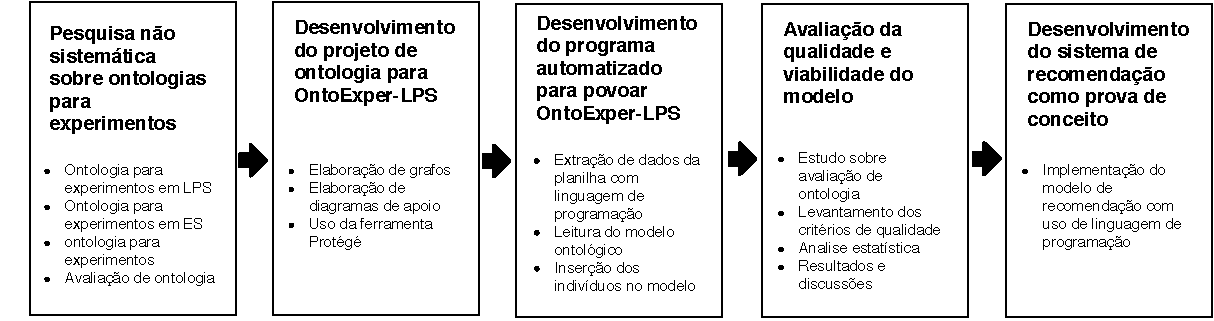
\includegraphics[scale=.75]{metodologia.pdf}}
	\label{fig:metodologia_flow}
	\source{O Autor}
\end{figure}

\begin{itemize}
	\item \textbf{Pesquisa n�o sistem�tica sobre ontologias para experimentos:} foram realizado estudos n�o sistem�ticos para encontrar trabalhos relacionados descrevendo ontologias para experimentos de ES e avalia��o de ontologia. Alguns estudos encontrados serviram de apoio � essa pesquisa, est�o descritos na Se��o \ref{sec:trabalhos_relacionados};
	
	\item \textbf{Desenvolvimento do projeto de ontologia:} trata do desenvolvimento da OntoExper-SPL, que incluiu realizar a escolha das tecnologias e ferramentas de constru��o de ontologia, como por exemplo o Prot�g�, envolver os \textit{stakeholders} no projeto com experi�ncia no dom�nio de experimenta��o, selecionar abordagens e modelos de ontologias relacionados, prototipa��o e diagrama��o do projeto;
	
	\item \textbf{Desenvolvimento do programa automatizado para povoar OntoExper-SPL:} refere-se ao processo de desenvolvimento do programa automatizado de povoamento da ontologia. Para isso foi necess�rio o uso de ferramentas, bibliotecas e linguagens de programa��o. Foram mais de 200 experimentos encontrados na literatura. Em seguida foi executado o programa de extra��o de dados, povoando a ontologia por meio dos metadados mais o programa de extra��o;
	
	\item \textbf{Avalia��o da qualidade e viabilidade do modelo:} refere-se ao estudo emp�rico, com objetivo de avaliar a qualidade da OntoExper-SPL. Para isso foi elaborado um question�rio com oito crit�rios de qualidade, enviado para especialistas responderem, e posteriormente realizada uma an�lise estat�stica das respostas, bem como pontos de melhorias encontrados durante a avalia��o; e
	
	\item \textbf{Desenvolvimento do prot�tipo de sistema de recomenda��o como prova de conceito:} ap�s processar os indiv�duos na OntoExper-SPL foi elaborado um prot�tipo de sistema de recomenda��o utilizando o modelos de recomenda��o \textit{Collaborative Filtering}, al�m de \textit{frameworks} e linguagens de programa��o.
\end{itemize}


\section{Organiza��o do texto}

Este cap�tulo apresentou a contextualiza��o desta disserta��o, a motiva��o e a justificativa, objetivos e metodologia. O restante da disserta��o est� estruturado da seguinte forma: o Cap�tulo \ref{sec:fundamentacao_teorica} apresenta a fundamenta��o te�rica sobre LPS, experimentos em ES, qualidade de experimentos em ES e ontologias; o Cap�tulo \ref{sec:ontologia} apresenta uma ontologia para experimentos de LPS - OntoExper-SPL, destacando desde a concep��o ao povoamento da ontologia proposta e pr�-an�lise de pontos de falha da ontologia; o Cap�tulo \ref{sec:avaliacao} apresenta uma avalia��o emp�rica sobre a qualidade da OntoExper-SPL por especialistas da �rea; o Cap�tulo \ref{sec:recsys} apresenta um sistema de recomenda��o para experimentos de LPS, usando como modelo de dados a OntoExper-SPL; e o Cap�tulo \ref{sec:conclusao} apresenta a conclus�o acerca deste trabalho e as suas contribui��es, limita��es e trabalhos futuros.



\chapter{Fundamentação Teórica}
\label{sec:revisao}

Este tópico apresenta conceitos fundamentais sobre Linha de Produto de Software, Experimento e \textit{Quasi}-Experimento em Engenharia de Software, Qualidade de Experimentos e \textit{Quasi}-Experimento em Engenharia de Software, Ontologia e Sistemas de Recomendação tradicional e voltado para Engenharia de Software.

\section{Linha de Produto de Software}
\label{sec:lin_prod_software}

Uma Linha de Produto de Software (LPS) é um conjunto de produtos que endereçam a um determinado segmento de mercado ou missão particular \cite{northrop2007framework}. Esse conjunto de produtos também é denominado família de produtos, no qual os membros desta família são produtos específicos gerados a partir da reutilização de uma infraestrutura comum, denominada núcleo de artefatos (\textit{Core assets}). 

O núcleo de artefatos é composto por um conjunto de características comuns chamadas de similaridades, e características variáveis chamadas de variabilidades \cite{van2007product}. Este núcleo forma a base da LPS que determina a Arquitetura de uma LPS, que são eles, componentes reusáveis, modelos de domínios, requisitos da LPS, planos de testes e modelos de características de variabilidades.

O modelo de características contém todas as características de uma LPS e os seus inter-relacionamentos. De acordo com \citeauthor{apel2013analytic}, "uma característica é um comportamento característico ou visível ao usuário final de um sistema de software". Uma característica pode ser obrigatória, opcional ou alternativa. O modelo de características representa as variabilidades e as variantes de uma LPS \cite{apel2013analytic}.

\begin{itemize}
	\item Variabilidades são descritas por: Ponto de variação que permite a resolução de variabilidades em artefatos genéricos de uma LPS, e; 
	\item Variante é representa pelos: os possessíveis elementos que podem ser escolhidos para resolver um ponto de variação.
\end{itemize}

Restrições entre variantes, estabelecem os relacionamentos entre uma ou mais variantes, com o objetivo de resolver seus respectivos pontos de variação ou variabilidade em um dado tempo de resolução \cite{halmans2003communicating}.

O \textit{MobileMedia} é um exemplo didático de LPS, o produto final é um software que gerencia as mídias de um aparelho celular. O núcleo de artefatos deve conter algumas das seguintes características, opções de criar, visualizar, remover e editar a legenda da imagem. As características variantes opcionais podem ser, a capturar uma nova imagem, ordenar e favoritar imagens. As características variantes alternativas podem ser os diversos tamanhos de tela. O produto final deve possuir ao menos uma variante alternativa.

\begin{figure}[htb]
	\centering					
	{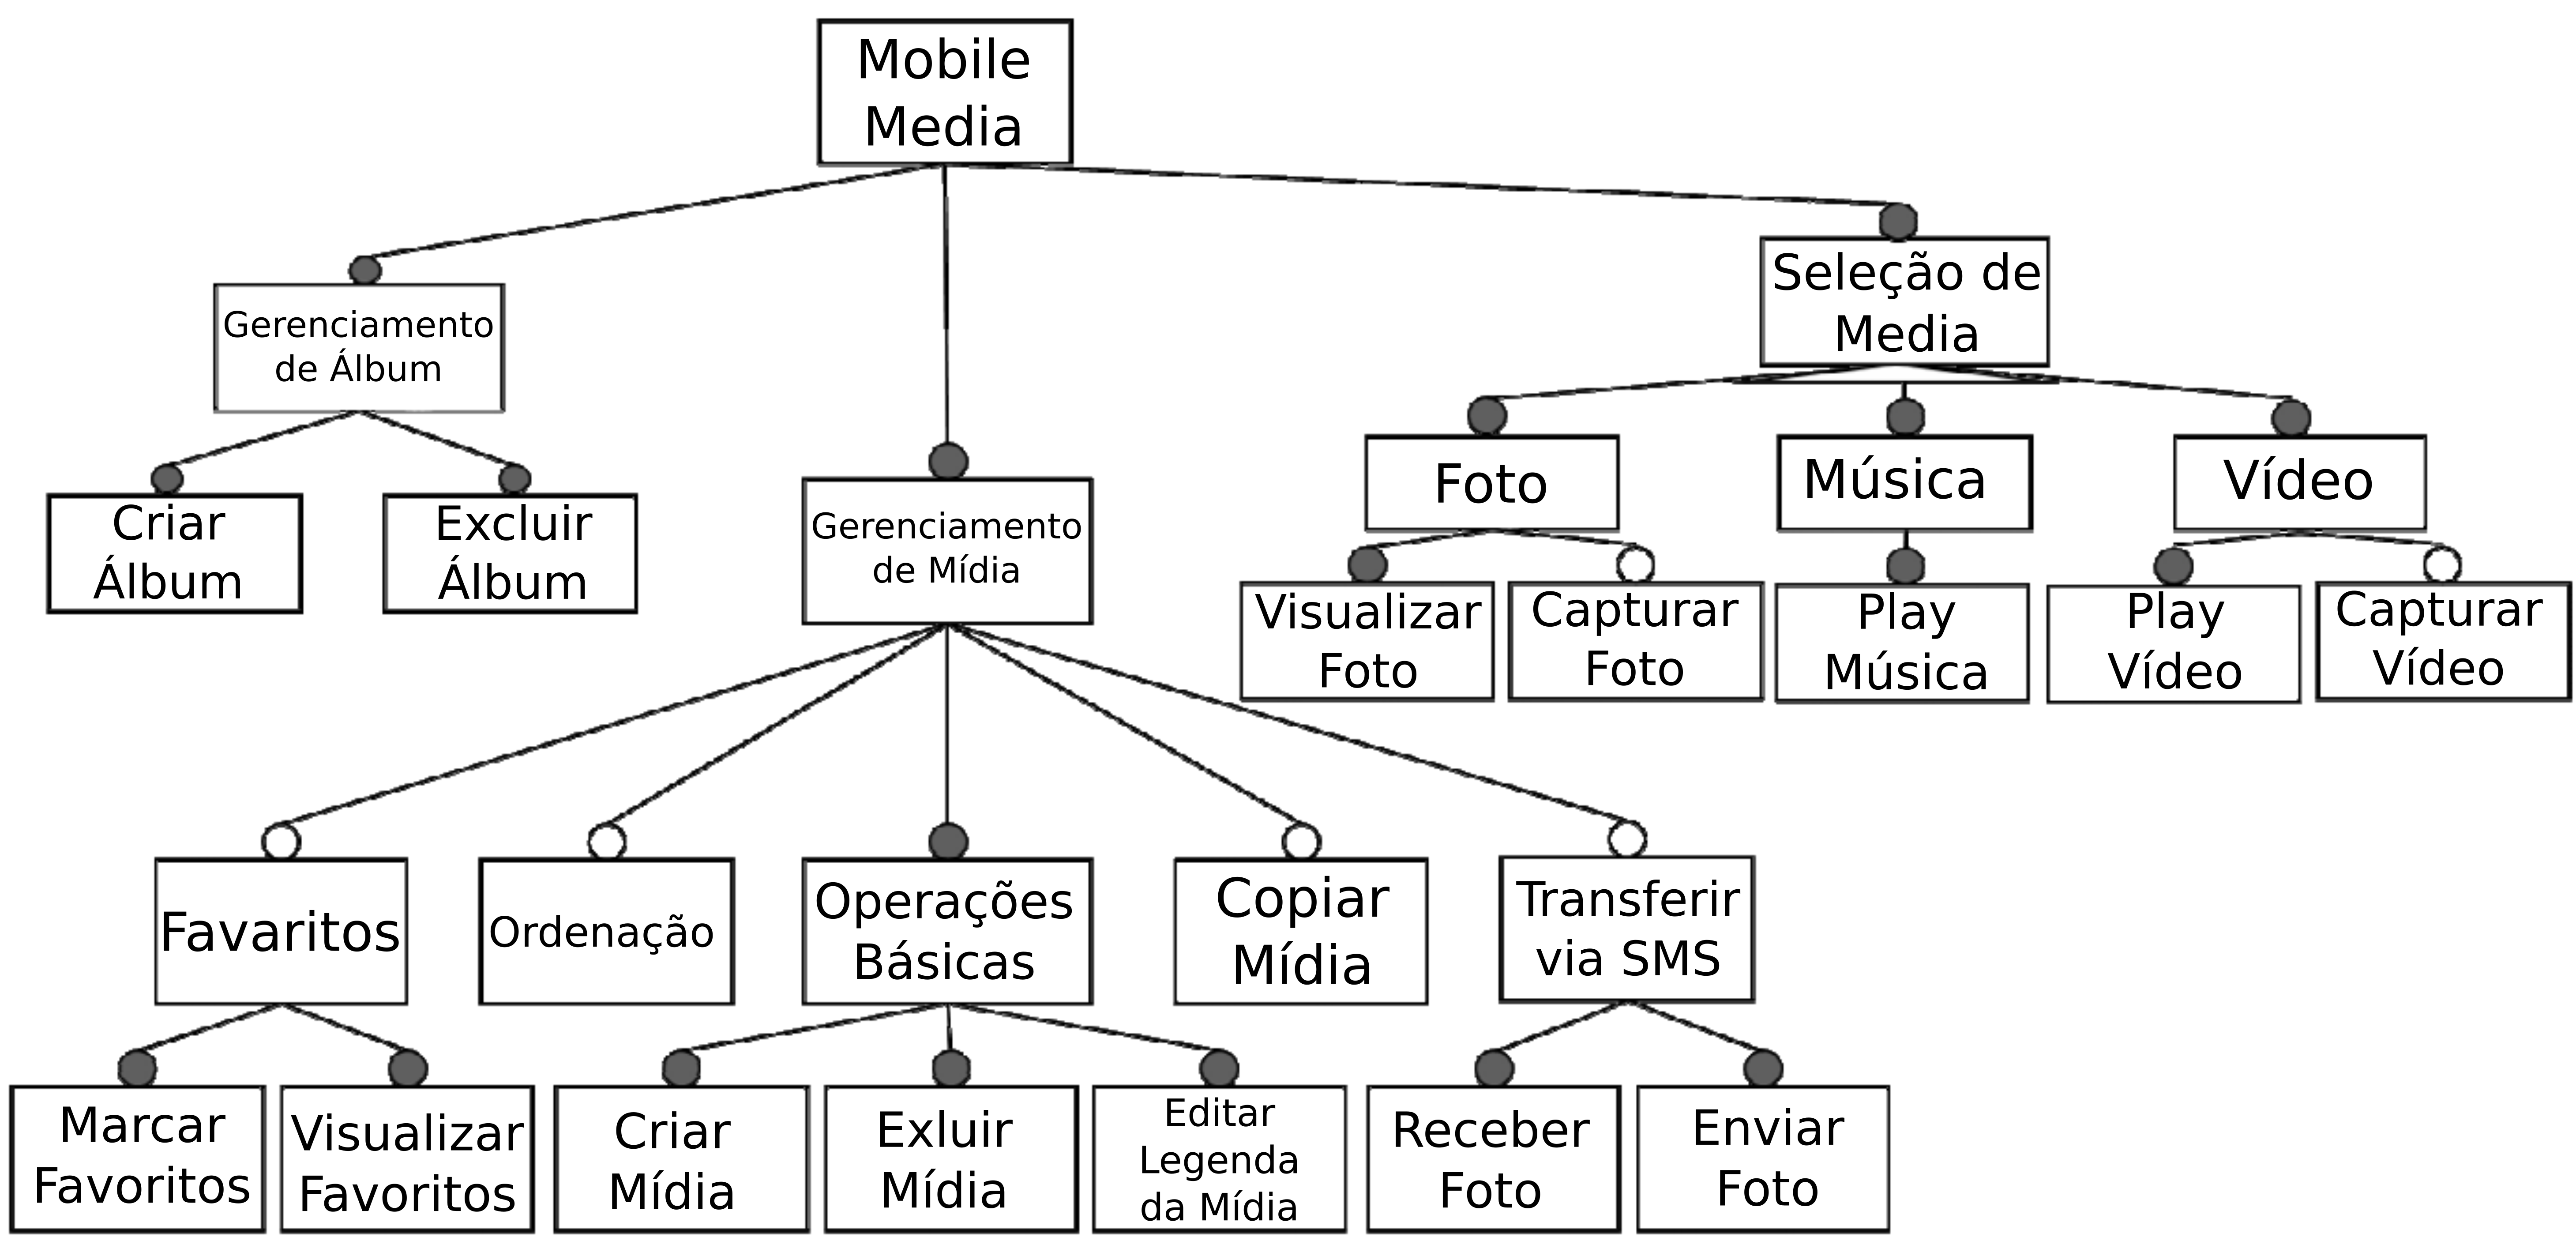
\includegraphics[scale=.33]{exemplo_lps_pt.png}}
	
	\caption{Um modelo de Características. Traduzido de \citet{sommerville2011software} }
	\label{fig:exemplo-lps}
\end{figure}

A \ref{fig:exemplo-lps} apresenta um grafo com o Modelo de Características da LPS \textit{MobileMedia}. As arestas com círculos preenchido representa as características pertencentes ao \textit{core asset}. As arestas com círculos vazios representa características opcionais. As arestas ligadas por um triangulo, como as que saem do vértice Seleção de Mídia, representam características alternativas, por exemplo, uma instância desta LPS deve possuir ao menos um tipo de seleção de mídia, seja ele, por Foto, Música ou Vídeo. 

Uma instancia deste exemplo teria as seguintes características no seu produto de software final:
\begin{itemize}
	\item Gerenciamento de Álbum; 
	\subitem Criar Álbum;
	\subitem Excluir Álbum;
	\item Gerenciamento de Mídia;
	\begin{itemize}
		\item Operações Básicas
		\subitem Criar Mídia
		\subitem Excluir Mídia
		\subitem Editar Legenda Mídia			
		\item Favoritos;
		\subitem Marcar Favoritos
		\subitem Visualizar Favoritos			
	\end{itemize}
	\item Seleção de Mídia;
	\subitem Foto
	\subitem Visualizar Foto
	\subitem Capturar Foto			
\end{itemize}

\citeauthor*{pohl2005software} desenvolveram o \textit{framework} para engenharia de LPS. O objetivo deste de \textit{framework} é incorporar os conceitos centrais da engenharia de linha de produto tradicional, proporcionando a reutilização de artefatos e a customização em massa por meio de variabilidades. O \textit{framework} está dividido em dois processos, o de Engenharia de Domínio e o de Engenharia de Aplicação, conforme apresentado na \ref{fig:framework-lps}.

\begin{itemize}
	\item \textbf{Engenharia de Domínio:} processo em que as similaridades e as variabilidades das LPSs são identificadas e realizadas. No qual, é composto de cinco subprocessos principais, sendo eles: Gerenciamento de Produto, Engenharia de Requisitos do Domínio, Projeto do Domínio, Realização do Domínio e Teste de Domínio;

	\item \textbf{Engenharia de Aplicação:} processo em que as aplicações de uma LPS são construídas por meio da reutilização de artefatos de domínio, explorando as variabilidades de uma linha de produto. No qual, é composto pelos subprocessos: Engenharia de Requisitos da Aplicação, Projeto da Aplicação, Realização da Aplicação e Teste da Aplicação.
\end{itemize}

\begin{figure}[htb]
	\centering					
	{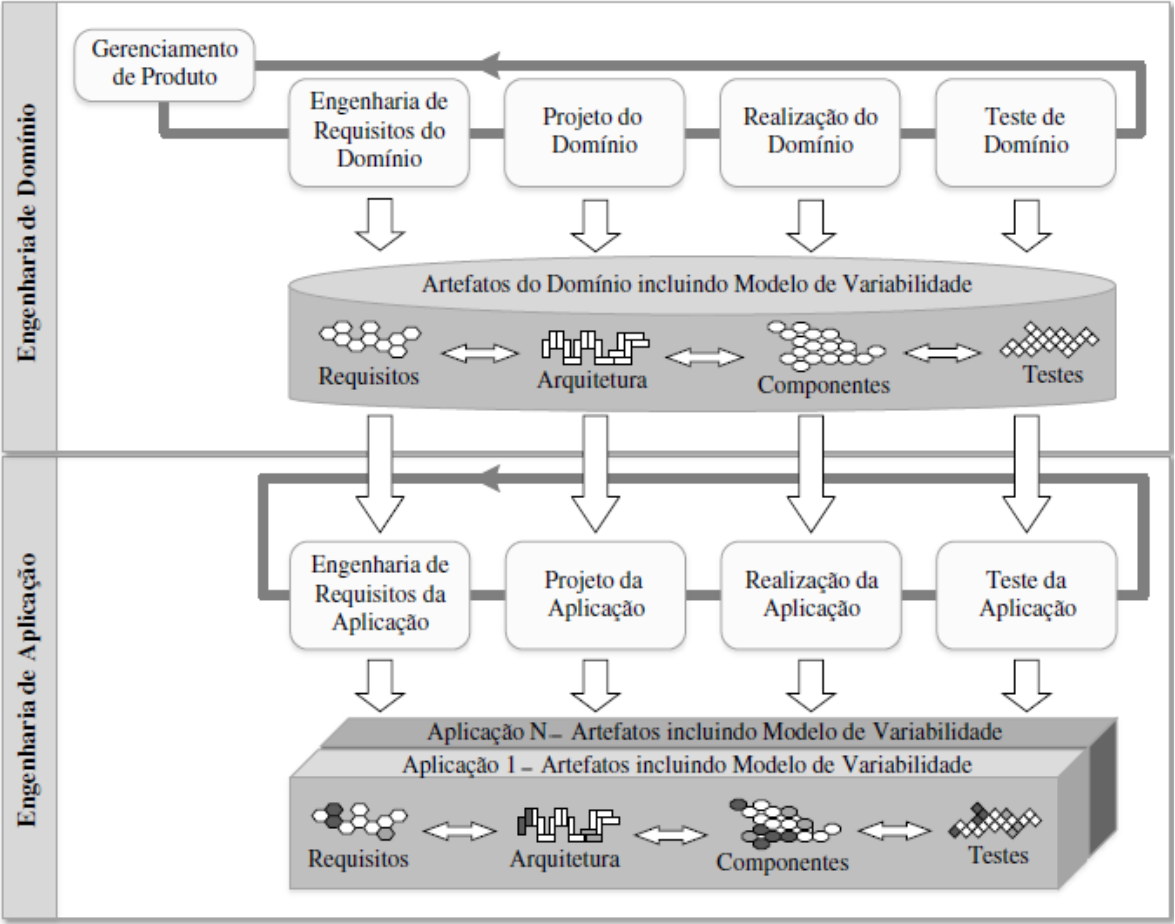
\includegraphics[scale=.37]{framewor_lps.png}}
	
	\caption{\textit{Framework} de Engenharia de LPS (Pohl et al., 2005). Traduzido por Geraldi (2015) }
	\label{fig:framework-lps}
\end{figure}


\section{Experimentos e \textit{Quasi}-Experimento em Engenharia de Software}
\label{sec:exp_eng_software}

Existe uma diferença relevante entre experimento e \textit{quasi}-experimento, esta diferença está relacionada a amostra do experimento. Quando se trata de um experimento a amostra é uma representação aleatória e válida de uma determinada população, ou seja, a amostra é uma representação da população. Quando se trata de \textit{quasi}-experimento a amostra não é aleatória e não representa sua população. É difícil realizar experimentos em LPS, devido a dificuldade de determinar uma amostra representativa e aleatória da população, pois normalmente estas amostras são pessoas \cite{wohlin2012experimentation}.

Por meio de um modelo teórico entre dois ou mais fenômenos relacionados a fim de determinar se este modelo proposto pode ser considerado correto, se desenvolve o experimento onde relacionamos a causa e o efeito deste modelo. Assim, utiliza-se o modelo para criar uma hipótese em relação às mudanças particulares nos fenômenos (a causa) que levarão a mudanças no outro (o efeito). Logo, o papel do experimento é testar a hipótese para decidir se é verdadeira ou falsa \cite{kitchenham2015evidence}. A \ref{fig:experimento} apresenta à ideia de uma relação causa e efeito em teoria, na qual a parte superior à linha trastejada se encontra a teoria e, na parte inferior a observação \cite{wohlin2012experimentation}.

\begin{figure}[htb]
	\centering					
	{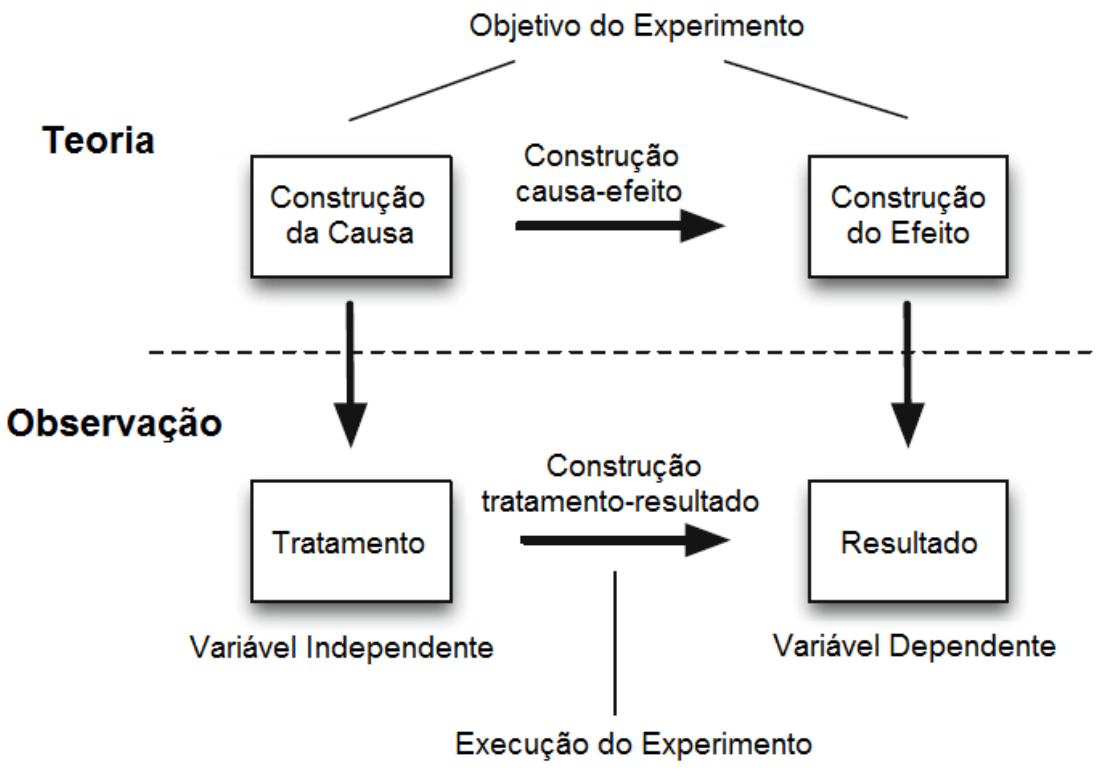
\includegraphics[scale=.37]{experimento.png}}
	
	\caption{Conceitos Essenciais de um Experimento. Traduzido de \citet{wohlin2012experimentation} }
	\label{fig:experimento}
\end{figure}

Um dos principais elementos de um experimento são as variáveis dependentes e independentes. 

\begin{itemize}
	\item \textbf{Variáveis independentes:} estão associadas à causa e controladas como resultado das atividades do experimentador, também são chamadas de fatores que podem assumir valores denominados tratamentos;
	\item \textbf{Variáveis dependentes:} estão associadas ao efeito e resultam nas mudanças que o experimentador realiza nas variáveis independentes \cite{kitchenham2015evidence}. 
\end{itemize}

Segundo \citealt{kitchenham2015evidence}, existe uma característica dita fator de confusão em experimentos de ES que envolvem seres humanos. Esse fator pode ser representado pela presença de algum elemento indesejável no estudo que dificulta distinguir entre duas ou mais causas possíveis de um efeito que foi medido pela variável dependente como, por exemplo, os níveis de habilidade dos participantes e a extensão de suas experiências anteriores com o objeto experimental.

Em Engenharia de Software, especialmente em LPS, é difícil de se executar experimentos dado que estes devem possuir aleatoriedade completa em suas variáveis. Isto se deve à dificuldade de alocar os participantes e/ou objetos a diferentes tratamentos de maneira aleatória, bem como, à falta de representatividade do número de participantes em uma amostra da população. Portanto, os experimentos realizados nesta área são, frequentemente, \textit{quasi}-experimentos, nos quais não há aleatoriedade dos participantes e/ou dos objetos experimentais, em ES chamados de artefatos de software, podendo ser processos ou ferramentas \cite{wohlin2012experimentation}.

Segundo \citealt{wohlin2012experimentation} a realização de um experimento pode ser dividido em um processo contendo cinco atividades, conforme apresentadas na \ref{fig:proc_exp} e descritas a seguir:

\begin{figure}[htb]
	\centering					
	{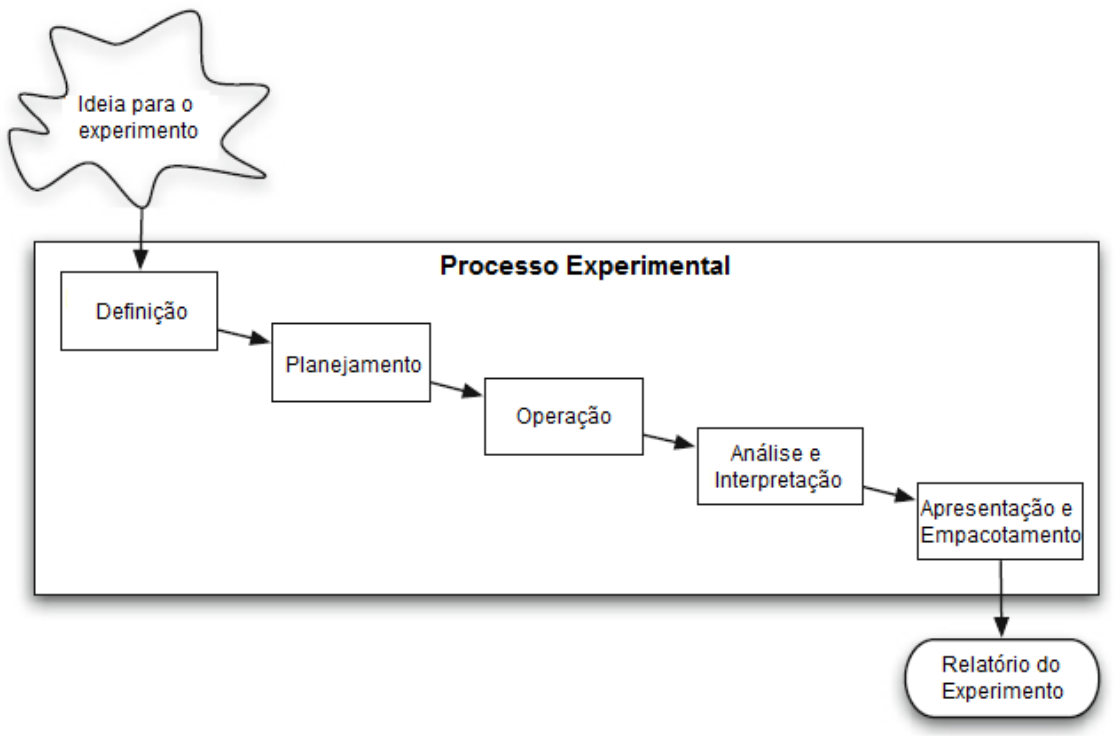
\includegraphics[scale=.37]{proc_exp.png}}
	
	\caption{Visão Geral do Processo Experimental. Traduzido de \citet{wohlin2012experimentation}}
	\label{fig:proc_exp}
\end{figure}


\begin{itemize}
	\item \textbf{Definição:} é a primeira atividade, onde define-se o problema, objetivo e metas do experimento. Caso não seja devidamente estabelecida, pode ocorrer retrabalho ou o experimento não pode ser utilizado para se estudar o que era almejado;

	\item \textbf{Planejamento:} é uma preparação de como o experimento será conduzido, em que ocorre a determinação do contexto do experimento, a formulação das hipóteses, sendo \textbf{hipótese nula} que o experimentador espera rejeitar com a maior confiança possível e a \textbf{hipótese alternativa} que se espera aceitar, a seleção de variáveis (dependentes e independentes), a seleção dos participantes, o projeto do experimento, a instrumentação e a avaliação da validade, dividida em quatro tipos, sendo \textbf{validade interna} refere-se ao relacionamento tratamento-resultado; \textbf{validade externa} apresenta a generalização dos resultados a uma população maior; \textbf{validade de \textit{constructo}} demonstra a relação entre a teoria e observação; e \textbf{validade de conclusão} refere-se a como os experimentadores foram aptos de analisar os resultados de um estudo e se a forma como foi feita é apropriada \cite{kitchenham2015evidence}.

	\item \textbf{Operação:} essa atividade é composta da \textbf{preparação} dos participantes e dos materiais necessários (instrumentação); \textbf{execução} das tarefas pelos participantes de acordo com diferentes tratamentos e coleta dos dados; e \textbf{validação dos dados} pelo experimentador, verificando os dados informados pelos participantes, de forma que os resultados do experimento sejam válidos; 
	
	\item \textbf{Análise e Interpretação:} os dados coletados na atividade anterior são analisados utilizando a estatística descritiva. Após isso, é verificada a necessidade de redução do conjunto de dados, de forma a garantir que os dados representam uma informação correta e/ou esperada. Por fim, realiza-se o teste de hipóteses para avaliar estatisticamente se hipótese nula pôde ser rejeitada. 
	
	\item \textbf{Apresentação e Empacotamento:} nessa atividade, os resultados são reportados, por exemplo, como artigos em conferência e/ou periódico, relatórios de tomada de decisão e empacotados para permitir a replicação do experimento, como material educativo, entre outros.
\end{itemize}

\section{Qualidade de Experimentos em Engenharia de Software}
\label{sec:qual_exp_eng_software}

Segundo \citet{dieste2013challenges}, o conceito de qualidade de experimentos em ES pode ser visto em dois pontos de vista diferentes, o primeiro é considerar a qualidade como o resultado da validade interna de um bom experimento e o segundo é tornar a qualidade operacional assim como a quantidade de vieses nos resultados experimentais. Outro ponto colocado por \citeauthor{dieste2013challenges}, é a validade externa que também tem uma função chave ao analisar se um experimento tem boa qualidade, porém essa função é contrária à validade interna.

Na \ref{tab:conceito_qualidade} são apresentadas as definições dos conceitos de qualidade citados anteriormente.

% Please add the following required packages to your document preamble:
% \usepackage{booktabs}
\begin{table}[]
	\centering
	\caption{Definições dos conceitos de qualidade em experimentos em Engenharia de
		Software. Traduzido de \citet{kitchenham2007large}}
	\label{tab:conceito_qualidade}
	\begin{tabular}{@{}lll@{}}
		\toprule
		Termo & Sinônimo & Definição \\ \midrule
		Viés & Erro sistemático & \begin{tabular}[c]{@{}l@{}}Uma tendência para produzir resultados \\ que partem sistematicamente de resultados \\ "verdadeiros". Resultados sem viés são\\ válidos internamente.\end{tabular} \\
		Validade Interna & Validade & \begin{tabular}[c]{@{}l@{}}O alcance em que o projeto e a condução \\ do estudo são possíveis de evitar erro sistemático. \\ A validade interna é um pré-requisito \\ para a validade externa.\end{tabular} \\
		Validade Externa & \begin{tabular}[c]{@{}l@{}}Generabilidade, \\ Aplicabilidade\end{tabular} & \begin{tabular}[c]{@{}l@{}}O alcance em que os efeitos observados no estudo \\ são aplicáveis fora do estudo.\end{tabular} \\ \bottomrule
	\end{tabular}
\end{table}

Segundo \citet{dieste2011systematic} os experimentos de boa qualidade são aqueles livres de vieses. O viés está relacionado com a validade interna, por exemplo, quão bem os experimentos são planejados, executados e analisados \cite{dieste2013challenges}. Para minimizar os vieses existem alguns métodos como, aleatorização para criar grupos experimentais homogêneos, imparcialidade para alocar os indivíduos. Desta forma os resultados podem ser analisados mesmo depois do experimento ter sido realizado com replicações. Enquanto os experimentos de baixa qualidade seriam os que usam pouco ou nenhum dos métodos citados \cite{dieste2011systematic}.

Como o viés não pode ser medido, existem algumas abordagens para avaliá-lo. Os instrumentos de Avaliação de Qualidade (AQ), são projetados para avaliar a validade interna e inferir a qualidade de experimentos, tais como, abordagens simples (questionários), \textit{checklists} (contem ou não contem), escalas de qualidade, opinião de especialista \cite{dieste2011systematic,dieste2013challenges,teixeira2014analise}.

Por outro lado a qualidade de um experimento em ES também pode ser avaliada considerando o projeto e análise dos experimentos, em termos de poder estatístico, análise do tamanho de efeito (resultado), \textit{quasi}-experimentais e relatório de experimento \cite{kampenes2007quality}.

Até o momento não se tem conhecimento de trabalhos que tratam a qualidade de experimentos em área especifica de ES. Entretanto, foram recuperados alguns trabalhos, por meio de pesquisas não sistemáticas, que estão relacionados com a avaliação de qualidade dos experimentos em Engenharia de Software, descritos a seguir:

\begin{itemize}
	\item \citet{kitchenham2007large} propõem um \textit{checklist} de avaliação de qualidade de experimentos em ES contendo cinquenta questões para avaliar a qualidade de experimentos, em que sugerem que os pesquisadores selecionem apenas as questões do \textit{checklist} mais adequadas ao contexto de suas próprias questões de pesquisa.
	
	\item \citet{kitchenham2015evidence} apresentam um \textit{checklist} de avaliação de qualidade de experimentos em ES com nove questões, onde cada questão possui subquestões	categorizadas em: (i) "Questões sobre objetivo", (ii) "Questões sobre o projeto, coleta de dados e análise do dados" e (iii) "Questões sobre o resultado do estudo".
	
	\item \citet{dieste2011systematic}  desenvolveram uma escala de qualidade para determinar a qualidade de experimentos, contendo dez questões baseadas nas cinco dimensões de \citet{kitchenham2007large}, sendo: contexto experimental, projeto experimental, análise, interpretação dos resultados e apresentação dos resultados. As respostas de cada questão são "sim" ou "não".	
\end{itemize}


\section{Ontologia}
\label{sec:ontologia}

A palavra ontologia é formada por meio dos termos gregos ontos (ser) e logos (estudo, discurso), que engloba algumas questões abstratas como a existência de determinadas entidades, o que se pode dizer que existe, qual o significado do ser, etc. Segundo \citet{wolff1962philosophia}, ontologia é um ramo da filosofia que estuda a realidade e existência, ou o ser enquanto ser. Em outras palavras, é o estudo da descrição de coisas do mundo real. Outro ponto de vista proposto por \citet{gruber1993ontology}, diz que ontologias são uma especificação formal de uma contextualização e uma contextualização é uma visão abstrata e simplificada do mundo.

Ontologia em Computação, Sistemas de Informação e Ciência da Informação, é definida como um modelo de dados que representa um conjunto de conceitos dentro de um domínio e os relacionamentos entre estes. Uma ontologia é utilizada para realizar inferência sobre os objetos do domínio. No cenário atual, as ontologia em ciências da informação são utilizadas como uma forma de representação de conhecimento lógico, possibilitando a inferência de novos fatos com base nos dados armazenados na ontologia.

Uma ontologia define primitivas/diretrizes de um domínio de conhecimento, estas primitivas/diretrizes podem ser definidas como classes, atributos, propriedades e restrições. Essas definições seguem o padrão de representação conhecido como lógica descritiva. A lógica descritiva representa os conceitos de um domínio (chamado de \textbf{TBox} - \textit{Terminological Box}) separadamente dos indivíduos (chamado de \textbf{ABox} - \textit{Assertion Box}) \cite{calvanese2005dl}. A lógica descritiva é mais representativa e eficiente que a lógica proposicional e a lógica de predicados (usados em linguagens de programação lógica, como Prolog).

Portanto uma ontologia para a representação de um conhecimento possui a seguinte estrutura: Uma base de conhecimento onde estão os dois conjuntos de conhecimento terminológico (\textbf{TBox}) e o conjunto de conhecimento sobre objetos (\textbf{ABox}), seguido de um mecanismo de inferência e uma aplicação para atuar na manipulação de informações extraídas do mecanismo de inferência, A \ref{fig:estrct_onto} apresenta essa estrutura.

\begin{figure}[htb]
	\centering					
	{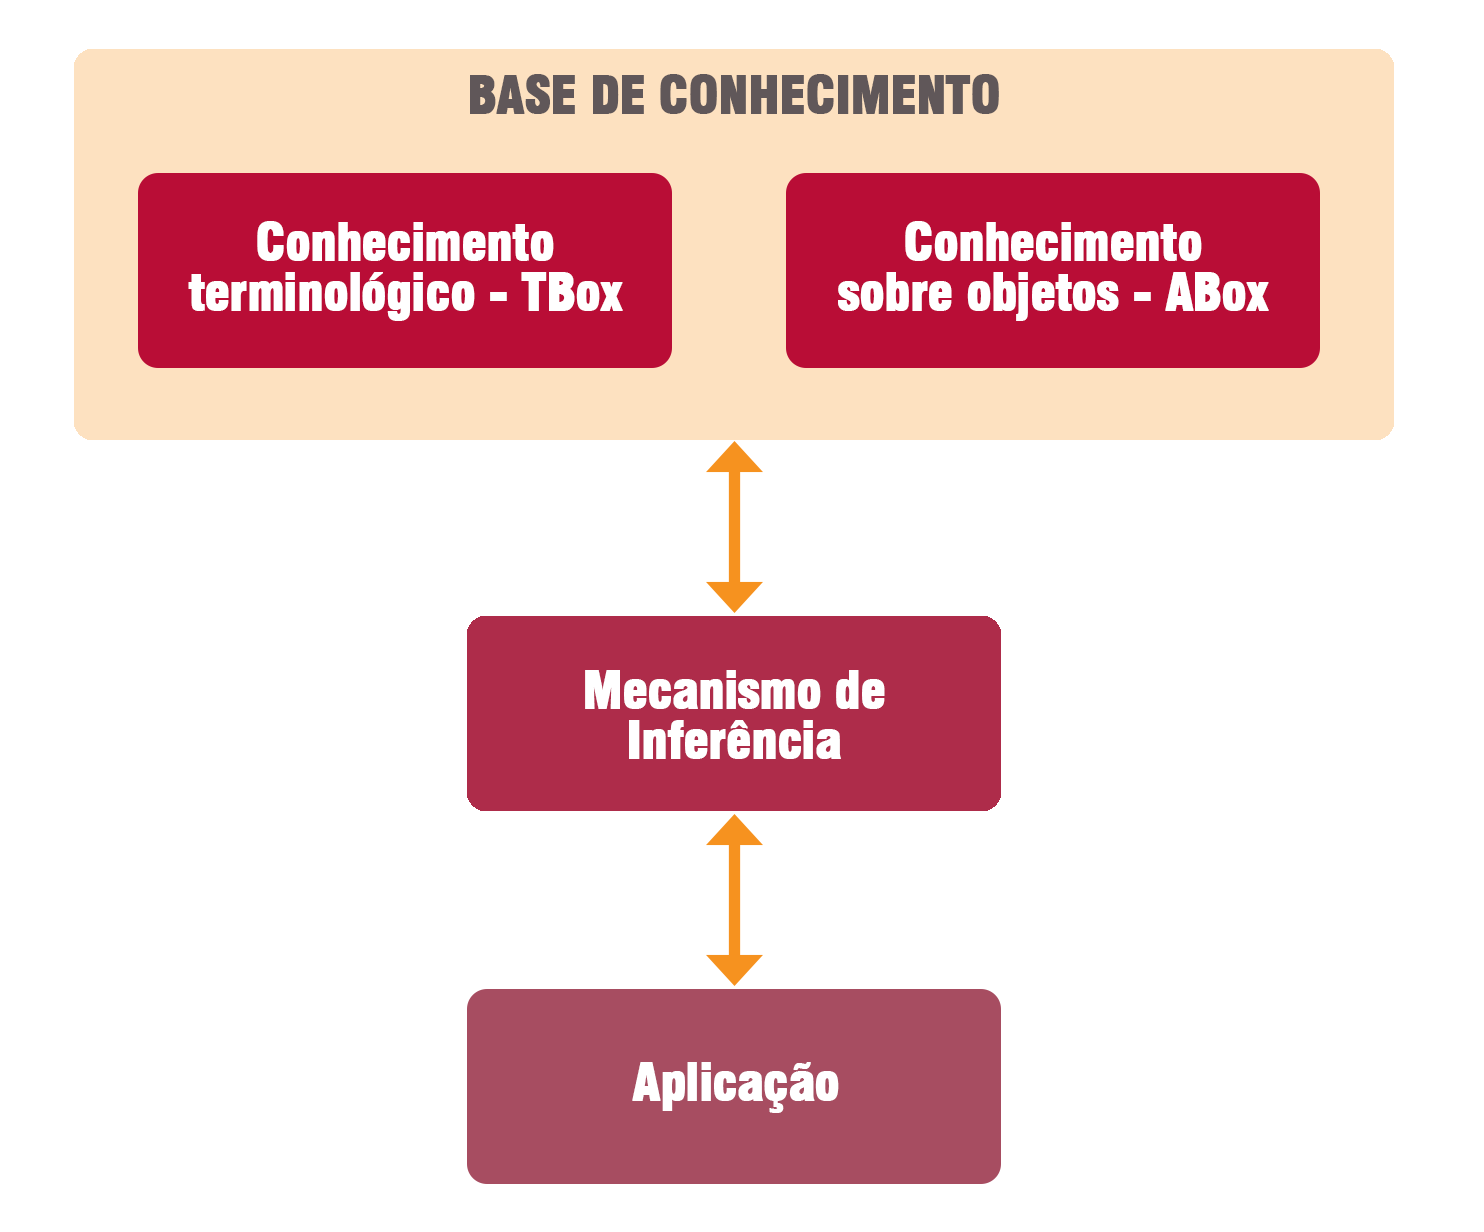
\includegraphics[scale=.7]{estrutura_ontologia.png}}
	
	\caption{Estrutura de uma Ontologia. Autor}
	\label{fig:estrct_onto}
\end{figure}

\begin{figure}[htb]
	\centering					
	{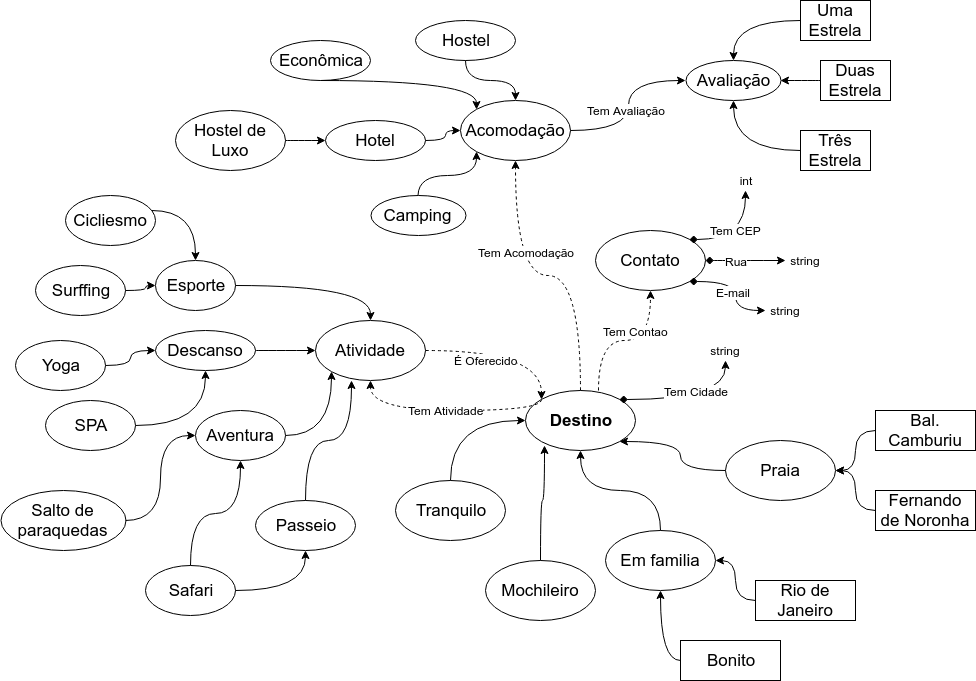
\includegraphics[scale=0.45]{exemplo_ontologia.png}}
	
	\caption{Exemplo de uma Ontologia para o domínio: Destino de Viagem. Autor}
	\label{fig:exemplo_ont}
\end{figure}

A \ref{fig:exemplo_ont} apresenta um exemplo de ontologia, por meio de um grafo, para o domínio: "destino de viagem". Os vértices ovais representam as classes, e os vértices retangulares representam os indivíduos (instâncias da classe). As arestas comuns representa um relacionamento de classe e subclasse, as arestas trastejadas representam um relacionamento de propriedade, já as arestas que começam com um losango indica a definição de uma propriedade, especificando sua tipagem.


\section{Sistema de Recomendação}
\label{sec:sit_recmendacao}

Os sistemas de recomendação são aplicativos de software que visam dar suporte para usuário na tomada de decisões ao interagir com grandes espaços de informação. Estes softwares recomendam itens de interesse para os usuários com base em preferências que tenham sido expressas explicitamente ou implicitamente \cite{ricci2011introduction}. Segundo \citet{mahmood2009improving} os sistemas de recomendação são técnicas ou ferramentas de software, que podem reduzir a sobrecarga de informações para os usuários, sugerindo itens, conteúdos ou serviços, entre outros.

\subsection{Sistemas de Recomendação Tradicional}

Os sistemas de recomendação surgiram nos trabalhos extensivos das ciências cognitivas, teoria de aproximação, recuperação da informação e teoria de previsões e também possuem influências das ciências de administração e marketing \cite{allen2001econometric, murthi2003role}. O primeiro sistema de recomendação proposto foi o \textit{Tapestry}, nesse sistema criou-se um modelo mais usados em sistemas de recomendação, onde a recomendação de conteúdo é auxiliada pela colaboração de um grupo de pessoas, batizada como "filtragem  colaborativa". Nesse trabalho, iniciou o desafio de casar corretamente os que dados recomendados com os usuários que o recebem, analisando o real relacionamento de interesse \cite{kwong1992dynamic, resnick1997recommender}.

Podemos apresentar uma definição formal para sistema de recomendação da seguinte forma: 

\newtheorem{mydef}{Definicão}
\begin{mydef}
	Seja $C$ o conjunto de todos os usuários de um determinado sistema, e seja $S'$ o conjunto de todos os possíveis itens que podem ser recomendados como livros, filmes, restaurantes etc. Seja $u$ a função utilidade que mede o quão útil é um determinado item s para um determinado usuário $c$, \textbf{\textit{u}:C x S $\rightarrow$ R}, onde $R$ é um conjunto totalmente ordenado segundo a função utilidade. Então, para cada usuário \textbf{\textit{c} $\in$ C}, procura-se um item \textbf{\textit{s'} $\in$ S} que maximiza a utilidade do usuário. Isto pode ser expressado pela equação \ref{eq:form_sis_rec}:
	
	\begin{equation}
	\label{eq:form_sis_rec}
	\forall c \in C, s'_{c} = argmax_{s \in S u(c, s)}
	\end{equation}
	
	Em um sistema de recomendação a utilidade de um item é geralmente representada por uma avaliação que indica o quanto um determinado usuário gosta de um item. No entanto, conforme descrito na definição acima, a função de utilidade pode ser uma função arbitrária.
	
	Cada elemento dos usuários $C$ pode ser definido por um perfil que inclui as características do usuário, por exemplo, a sua idade, sexo, etc. No caso mais simples, o perfil pode conter um único elemento como um identificador único (ID). Da mesma forma, cada item de $S$ pode ser definido por um conjunto de características. Por exemplo, na recomendação de filmes, na qual $S$ é a coleção de filmes, cada filme pode ser representado não apenas pelo seu ID, mas também pelo seu título, gênero, diretor, ano de lançamento, etc.
\end{mydef}

Exitem cinco abordagens mais usadas em sistemas de recomendação, três tradicionais: Filtragem Colaborativa (\textit{Collaborative Filtering}), Filtragem Baseada em Conteúdo (\textit{Content-based Filtering}) e Recomendação Baseada no Conhecimento (\textit{Knowledge-Based Recommendation}), e duas modernas: Sistemas de Recomendação Híbridos \textit{(Hybrid Recommender Systems}) e Sistemas de Recomendação usando Informações de Contexto (\textit{Context-aware Recommender Systems}).

\begin{itemize}
	\item \textbf{\textit{Collaborative Filtering}:}
	A Filtragem Colaborativa baseia-se na ideia de "boca-a-boca" em que a informação passada de pessoa a pessoa desempenha um papel importante ao tomar uma decisão. Abstraindo, as pessoas são substituídas pelos chamados vizinhos mais próximos (NN) que são usuários com um padrão de preferência ou comportamento semelhante ao usuário atual. \cite{robillard2010recommendation}. Filtragem Colaborativa depende de dois tipos diferentes de dados: (1) um conjunto de usuários e (2) um conjunto de itens. A relação entre usuários e itens é expressada principalmente em termos de \textit{ratings} fornecidos pelos usuários e explorados em futuras sessões de recomendação para prever a classificação de um usuário \cite{robillard2010recommendation}.
	
	\item \textbf{\textit{Content-based Filtering}:}
	A Filtragem Baseada em Conteúdo tem como característica principal o pressuposto de interesses pessoais, por exemplo, os usuários interessados no tópico de qualidade de experimentos em LPS normalmente não alteram seu interesse de um dia para outro, mas também estarão interessados em um tópico próximo, como por exemplo experimentos em Sistema de Sistemas. Abstraindo, as abordagens de recomendação baseadas em conteúdo são aplicadas, por exemplo, quando se trata da recomendação de sites (notícias com conteúdo semelhante em comparação com o conjunto de notícias já consumidas) \cite{robillard2010recommendation}. Filtragem Baseada em Conteúdo depende de dois tipos diferentes de dados: (i) um conjunto de usuários e (ii) um conjunto de categorias (ou palavras-chave) atribuídas ou extraídas dos itens (descrições de itens). Os sistemas de recomendação de filtragem baseados em conteúdo calculam um conjunto de itens que são mais parecidos com itens já conhecidos pelo usuário atual \cite{robillard2010recommendation}.

	\item \textbf{\textit{Knowledge-Based Recommendation}:} 
	A recomendação baseada no conhecimento, baseia-se nos seguintes	dados básicos: (i) um conjunto de regras (restrições) ou métricas de similaridade e (ii) um conjunto de itens. Dependendo dos requisitos do usuário, regras (restrições) que descrevam quais itens devem ser recomendados. O usuário atual articula suas necessidades (preferências) em termos de especificações e propriedades de itens que são internamente bem representados em termos de regras (restrições).
	
	\item \textbf{\textit{Hybrid Recommender Systemson}:}
	São algoritmos que combinam \textit{Collaborative Filtering} com \textit{Content-based Filtering} e podem ser feitos de diversas formas diferentes, por exemplo, aplicando os dois separados e juntando os resultados depois, adicionando a saída de um ao outro ou unificando as duas abordagens em um único modelo. Alguns exemplos são as abordagens baseada em pesos, misturadas a cascatas \cite{jannach2010recommender}.
	
	
	\item \textbf{\textit{Context-aware Recommender Systems}:} 
	Existem casos de recomendações que não podem levar em consideração somente os dados do item ou do usuário, como conteúdo personalizado de um site de filmes, sites de viagens e até sites de notícias. A incorporação do contexto permite personalizar ainda mais a recomendação e criar experiências realmente válidas ao usuário. Segundo \citet{rahman2013ide} \textit{Context-aware Recommender Systems}, segue as abordagens anteriores assumindo a existência de certos fatores contextuais como, por exemplo, o tempo e a localização, que identificam o contexto no qual as recomendações são fornecidas. Eles assumem que cada um desses fatores contextuais podem ter uma estrutura. O fator Tempo, por exemplo, pode ser definido em termos de segundos, minutos, horas, dias, meses e anos. \citet{rahman2013ide} cita como classificar o contexto baseando-se nos seguintes aspectos, (i) o que um sistema de recomendação pode saber sobre esses fatores contextuais e (ii) como os fatores contextuais mudam ao longo do tempo. Desta forma podemos definir este tipo de sistema de recomendação pela formula \ref{eq:form_sis_rec_ca}
	
	\begin{equation}
		\label{eq:form_sis_rec_ca}
		f:User \times Item \times Context \rightarrow Rating
	\end{equation}

\end{itemize}


\subsection{Sistema de Recomendação em Engenharia de Software}

Em Engenharia de Software (\textit{Recommendation System in Software Engineering} - RSSEs), sistemas de recomendação desempenham importantes funções a fim de ajudar a equipe de software a lidar com sobrecarga de informações, filtrando e fornecendo informações úteis. São ferramentas de software introduzidas especificamente para ajudar equipes de desenvolvimento de software e partes interessadas a lidar com a busca de informações em um determinado contexto em ES \cite{robillard2010recommendation}.

\citet{robillard2010recommendation} comenta que, em um ambiente de desenvolvimento de software aplicando ES existe um \textit{landscape} de informações sobre o projeto em desenvolvimento, e este espaço de informações pode ser categorizados por:

\begin{itemize}
	\item Código fonte do projeto;
	\item História do projeto;
	\item Arquivos de comunicação;
	\item Dependências de API em outras fontes;
	\item Ambiente de desenvolvimento;
	\item Logs de interação entre os usuários;
	\item Logs de execução e;
	\item A web.
\end{itemize}

Um RSSE pode trazer simultaneamente dois aspectos distintos: (i) novidade e surpresa, porque as RSSEs ajudam a descobrir novas informações e (ii) traz familiaridade e reforço, pois as RSSEs suportam a confirmação do conhecimento existente. Finalmente, referenciar uma tarefa e um contexto específicos, distingue RSSEs de ferramentas de pesquisa genéricas, por exemplo, uma ferramentas de RSSR para ajudar os desenvolvedores a encontrar exemplos de código fonte \cite{robillard2010recommendation}.

RSSE compreende três componentes principais, (i) um mecanismo para coletar dados, (ii) um mecanismo de recomendação para analisar dados e gerar recomendações e (iii) uma interface de usuário para fornecer recomendações \cite{rahman2014towards}.

\begin{figure}[htb]
	\centering					
	{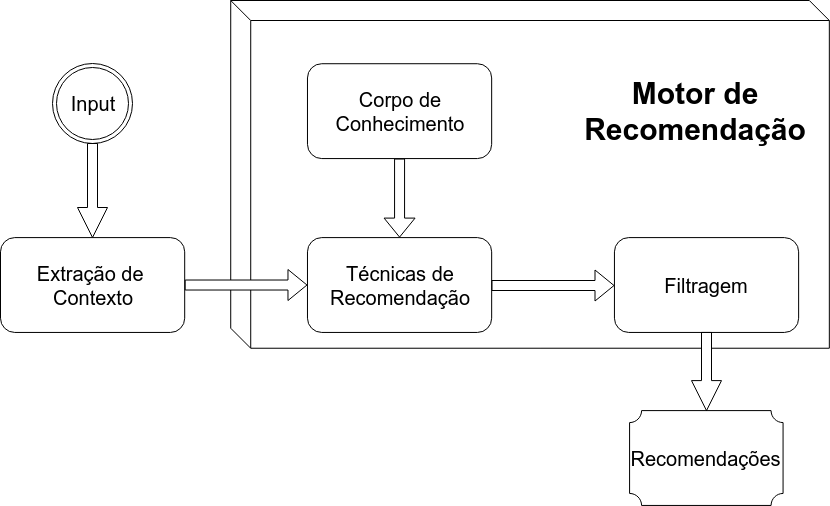
\includegraphics[scale=.5]{rsse.png}}
	
	\caption{Passos de Construção para um RSSE. Traduzido e Adaptado de \citet{maki2016systematic}}
	\label{fig:rsse}
\end{figure}

A \ref{fig:rsse} apresenta de forma geral como é construído um RSSE, partindo da entradas dos dados pelo \textit{input}, passando pela extração de contexto, seguindo para aplicação de alguma técnica de recomendação, na qual sofre um inferência do corpo de conhecimento (normalmente especifico para cada área de ES), depois segue pra um processo de filtragem dos resultados, e como saída a recomendação em si.

Foi encontrado uma revisão sistemáticas (trabalho da \citealp{maki2016systematic}), que aborda métodos e modelos de implementação de um RSSE apresentando vários aspectos de SR em ES, principalmente no tipo de corpo de conhecimento aplicado a RSSE. Nessa revisão foi possível identificar algumas áreas da ES que utiliza SR, apresentadas a seguir.

\begin{itemize}
	\item SR para exploração código fonte;
	\item SR para reuso de software;
	\item SR para refatoração de código fonte (por exemplo, \textit{class} em POO);
	\item SR para reuso de componentes de software;
	\item SR na exploração de APIs;
	\item SR na depuração de código (\textit{debugging})
	\item SR na recomendação de agentes \textit{Agile}
	\item SR na descoberta de requisitos;
	\item SR na mudança do ciclo de vida;
	\item SR na evolução do ciclo de vida e;
	\item SR na busca de \textit{bugs}.
\end{itemize}

Por meio deste estudo, foi possível identificar em qual domínio de aplicação da industria de ES estão aplicando qual técnica de SR, apresentados na \ref{tab:tec_x_doman} a seguir.

\begin{table}[]
	\centering
	\caption{Sumário de técnicas de recomendação em cada domínio, Traduzido e Adaptado de \citet{maki2016systematic} }
	\label{tab:tec_x_doman}
	\begin{tabular}{@{}llllllllll@{}}
		\toprule
		\multicolumn{1}{c}{\textbf{Domínios}} & \multicolumn{8}{c}{\textbf{Técnicas}} & \multicolumn{1}{c}{\textbf{\begin{tabular}[c]{@{}c@{}}Número de \\ Referências\end{tabular}}} \\ \midrule
		& CBF & CF & KBF & Hibrido & IA & \begin{tabular}[c]{@{}l@{}}Redes \\ Sociais\end{tabular} & \begin{tabular}[c]{@{}l@{}}Info. de\\ Contexto\end{tabular} & \begin{tabular}[c]{@{}l@{}}Grupo de \\ agregação\end{tabular} &  \\ \midrule
		Governo & 1 & 5 & 1 & 5 & 4 &  &  &  & 9 \\
		Negócios &  & 1 & 3 & 3 & 4 &  &  &  & 5 \\
		Comercio & 3 & 1 & 4 & 1 & 4 & 2 &  &  & 8 \\
		Livraria & 2 & 2 &  & 3 & 1 &  &  &  & 6 \\
		Escolas & 2 &  & 11 &  & 1 &  &  &  & 10 \\
		Turismo & 5 & 9 & 9 & 9 & 2 & 2 & 11 &  & 18 \\
		Pesquisa & 9 & 16 & 6 & 15 & 3 & 1 & 1 &  & 27 \\
		\begin{tabular}[c]{@{}l@{}}Grupo de \\ Atividade\end{tabular} & 9 & 5 & 2 & 5 & 8 &  &  & 2 & 21 \\
		\textbf{Total} & \textbf{31} & \textbf{39} & \textbf{36} & \textbf{41} & \textbf{27} & \textbf{5} & \textbf{12} & \textbf{2} & \textbf{104} \\ \bottomrule
	\end{tabular}
\end{table}

\section{Trabalhos Relacionados}

Até o momento não há trabalhos de sistema de recomendações para recomendar experimentos em ES, nem em LPS. Outros trabalhos relacionados mais próximos já foram apresentado na Seção 2.3 e não são objetos de evolução de experimento gerais em ES.

Encontramos alguns estudos que propuseram abordagens para representar formalmente dados sobre experimentos de SE.

A revisão da literatura mostrou que a maioria dos estudos focalizou a representação de todo o domínio do SE. Isso é muito complexo devido à quantidade de detalhes de cada campo. Em vez disso, nos concentramos primeiro em um campo de SE devido à nossa experiência em grupo.

Durante nossa revisão de literatura encontramos: \cite{garcia2008ontology} Ontologia para Experimentos Controlados em Engenharia de Software, \cite{scatalon2011packaging} Empacotando Experimentos Controlados Usando uma Abordagem Evolutiva Baseada em Ontologia (S), \cite{da2012foundational} Uma Ontologia Fundamental para Apoiar Experimentos Científicos, \cite{blondet2016ode} ODE: uma Ontologia para Projeto Numérico de Experimentos, \cite{soldatova2006ontology} Uma Ontologia de Experimentos Científicos, \cite{gelernter2016challenges} Desafios na Avaliação de Ontologia, \cite{cruzes2007extracting} Extraindo Informações da Engenharia de Software Experimental papéis. No entanto, todos esses trabalhos não tratam experimentos de SPL.

O trabalho de Garcia et al. \cite{garcia2008ontology}, Poveda-Villalón et al. \cite{scatalon2011packaging} e Cruz et al. \cite{da2012foundational} se destaca em nosso contexto por propor e modelar ontologias específicas para experimentos em engenharia de software. O trabalho de \cite{garcia2008ontology} propõe, através de diagramas de classes UML, uma ontologia para experimentos controlados em engenharia de software denominada EXPEROntology. Com o objetivo de ser uma ferramenta de transferência de conhecimento para auxiliares de pesquisadores e revisores, além de propor meta-análises, conduzir e avaliar experimentos controlados. O trabalho de Poveda-Villalón et al. \cite{scatalon2011packaging} é uma evolução do trabalho de Garcia et al. \cite{garcia2008ontology}, mas focado na evolução desta ontologia proposta. O trabalho de Cruz et al. \cite{da2012foundational} apresenta uma ontologia chamada OVO (Open onVence Ontology) na qual é inspirada por três teorias: (i) O ciclo de vida de experimentos científicos, (ii) Open Provent (OPM) e (iii) Unified Foundational Ontology ( OVNI) Este modelo OVO pretende ser uma referência para modelos conceituais que podem ser usados ??por pesquisadores para explorar a semântica de metadados.

Por outro lado, os trabalhos de Blondet et al. \cite{blondet2016ode} e Soldatova e King \cite{soldatova2006ontology} tratam ontologias no contexto geral de experimentos. O trabalho de Blondet et al. \cite{blondet2016ode} traz uma proposta de ontologia para DoE (Designs of Experiments) para apoiar as decisões de processo sobre o DoE. O trabalho de Soldatova e King \cite{soldatova2006ontology} propõe a ontologia da EXPO que é uma mediana da ontologia SUMO (Suggested Upper Merged Ontology). Esta ontologia visa especificar os experimentos formalizando e generalizando os conceitos de design, metodologias e representação de resultados. Este trabalho é o único que usa o modelo OWL-DL para representar a ontologia.

O trabalho de Gelernter e Jha \cite{gelernter2016challenges} dá uma visão geral sobre os desafios de avaliar uma ontologia, mas não trata da ontologia para experimentos.

Finalmente, o trabalho de Cruzes et al. \cite{cruzes2007extracting} trata de uma técnica para extrair meta-informação de experimentos em engenharia de software, entendemos que este assunto está relacionado a este artigo, pois estaremos gerando através da ontologia proposta diversos metadados sobre experimentos em SPL.

A revisão da literatura mostrou que a maioria dos estudos focalizou a representação de todo o domínio do SE. Isso é muito complexo devido à quantidade de detalhes de cada campo. Em vez disso, nos concentramos primeiro em um campo de SE devido à nossa experiência em grupo.
\chapter{Uma Ontologia para Experimentos em LPS (SMartOntology)}
\label{sec:ontologia}

Este tópico apresenta conceitos fundamentais sobre a proposta de ontologia SMartyOntology. Inicialmente foi realizado um processo de concepção do modelo em seguida foi desenvolvido o projeto desenvolvido se obter modelo. Com a finalidade de avaliação foi desenvolvido um exemplo de aplicação por meio de uma predição de recomendação qual artefato de LPS pode ser usado por um dado templete de experimento. Ao final desse capitulo foi realizado uma avaliação empírica do modelo, por meio de uma ferramenta que avalia pontos de falha do modelo.

\section{Concepção}
\label{sec:concepcao}

Com base na tipologia proposta por \cite{almeida2003visao} definimos o tipo de ontologia proposto na Tabela \ref{tab:type_ontology}:

\begin{table}[]
	\caption{Type of the Proposed Ontology}
	\label{tab:type_ontology}
	\begin{tabular}{@{}lll@{}}
		\toprule
		Approach & Rating & Description \\ \midrule
		\begin{tabular}[c]{@{}l@{}}As for the Mizoguchi function; \\ Vanwelkenbuyse; Ikeda (1995)\end{tabular} & \begin{tabular}[c]{@{}l@{}}Domain ontologies\end{tabular} & \begin{tabular}[c]{@{}l@{}}Reusable in the domain, they provide vocabulary \\ about concepts and their relationships, about the \\ activities and rules that govern them\end{tabular} \\
		\begin{tabular}[c]{@{}l@{}}As for the degree of Uschold formalism; \\ Gruninger (1996)\end{tabular} & Semi-formal & \begin{tabular}[c]{@{}l@{}}Expressed in natural language in a restricted \\ and structured way\end{tabular} \\
		\begin{tabular}[c]{@{}l@{}}As for the Jasper application; \\ Uschold (1999)\end{tabular} & \begin{tabular}[c]{@{}l@{}}Ontologies as specification\end{tabular} & \begin{tabular}[c]{@{}l@{}}An ontology is created for a domain, which is used \\ for documentation and maintenance in the \\ development of software.\end{tabular} \\
		\begin{tabular}[c]{@{}l@{}}As for the Haav structure; \\ Lubi (2001)\end{tabular} & \begin{tabular}[c]{@{}l@{}}Domain ontologies\end{tabular} & \begin{tabular}[c]{@{}l@{}}Describe vocabulary related to a domain, \\ such as medicine or automobiles\end{tabular} \\
		\begin{tabular}[c]{@{}l@{}}As for Van-Heijist content; \\ Schreiber; Wielinga (2002)\end{tabular} & \begin{tabular}[c]{@{}l@{}}Knowledge modeling ontologies\end{tabular} & \begin{tabular}[c]{@{}l@{}}Specify knowledge conceptualizations, have a \\ semantically rich internal structure, and are refined \\ for use in the domain of knowledge they describe\end{tabular} \\
		& \begin{tabular}[c]{@{}l@{}}Application ontologies\end{tabular} & \begin{tabular}[c]{@{}l@{}}Contains the definitions needed to model knowledge\\ in an application\end{tabular} \\
		& \begin{tabular}[c]{@{}l@{}}Domain ontologies\end{tabular} & \begin{tabular}[c]{@{}l@{}}Express concepts that are specific to a \\ given domain of knowledge\end{tabular} \\ \bottomrule
	\end{tabular}
\end{table}

Ou seja, quanto à função é uma ontologia de domínio, quanto ao grau de formalismo é uma ontologia semi formal, quanto à aplicação é uma ontologia de especificação, quanto à estrutura é uma ontologia de domínio e quanto ao conteúdo é tanto uma ontologia para modelagem de conhecimento quanto para aplicação e de domínio.

Foi aplicado o seguinte processo de elaboração da ontologia \cite{fernanda2007modelagem}:

\begin{itemize}
	\item Definição e estruturação dos termos por meio de classes;  
	\item Estabelecimento de propriedades (atributos) inerentes ao conceito representado por um termo;
	\item Povoamento da estrutura que satisfaçam um conceito e as suas propriedades;  
	\item Estabelecimento de relações entre os conceitos;
	\item Elaboração de sentenças para restringir inferências de conhecimento baseadas na estrutura.
\end{itemize}

Inicialmente foi desenvolvido um grafo para o modelo inicial da ontologia SMartyOntology, principalmente para validar os termos por meio de classes, subclasses e os relacionamento entre elas.

\begin{figure}[ht]
	\centering 
	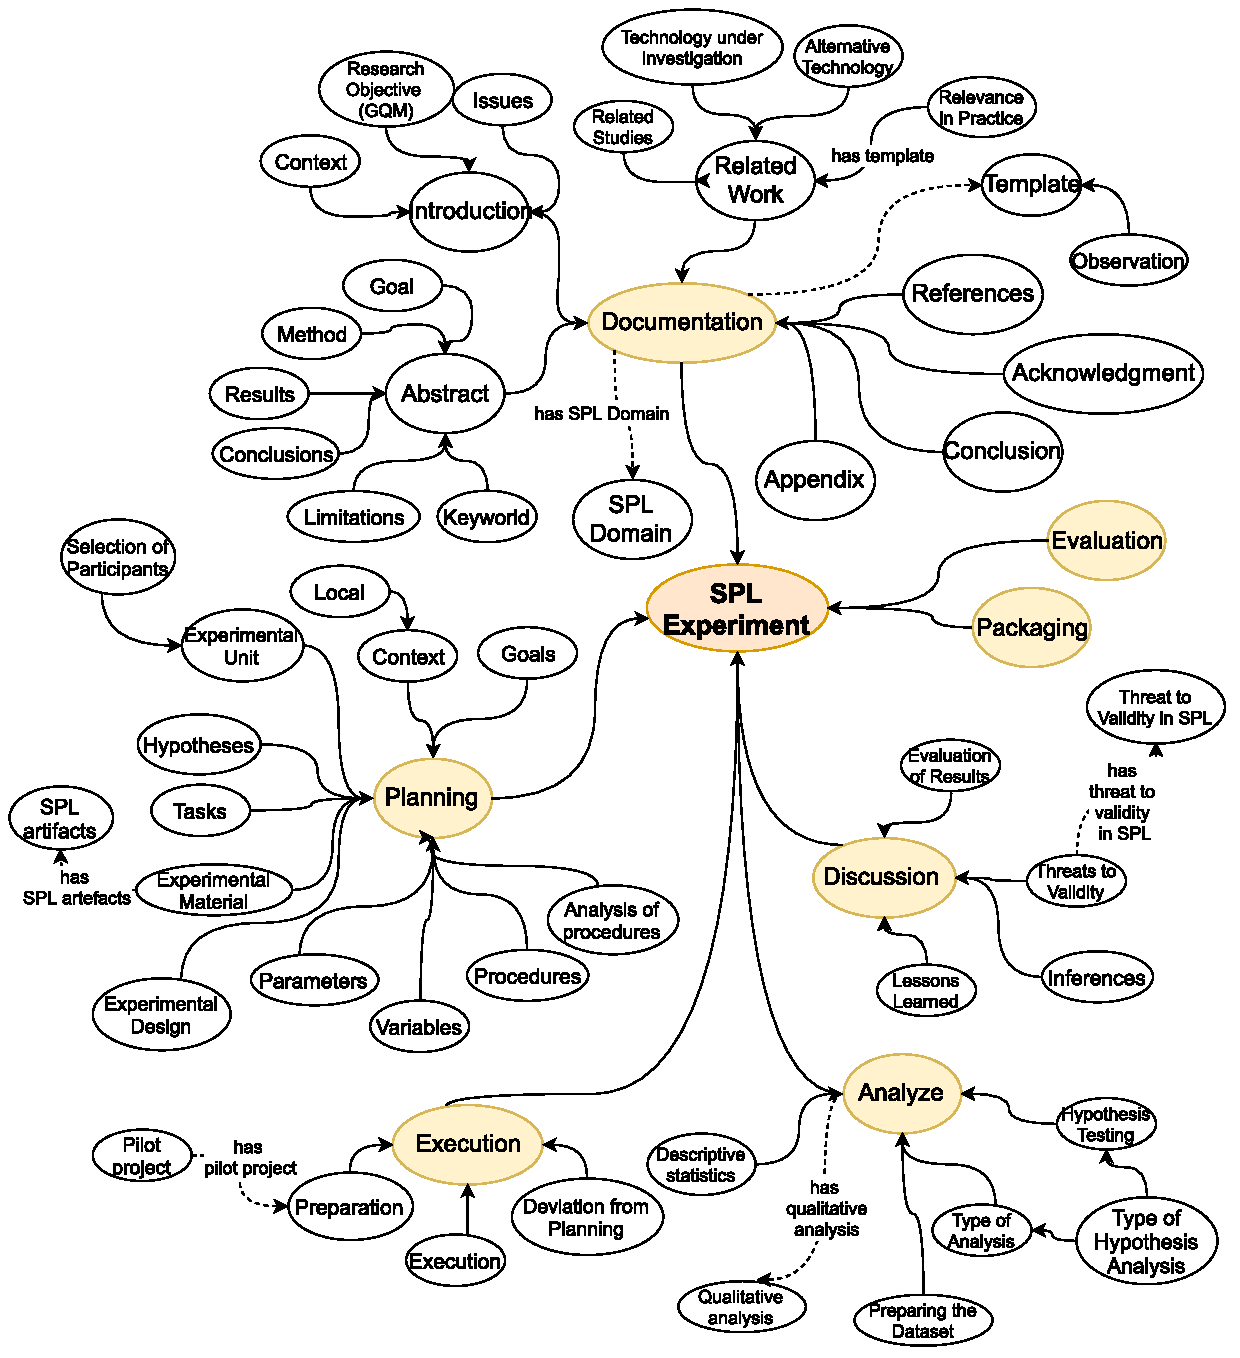
\includegraphics[width=11cm]{graph-all-class.pdf}
	\caption{Initial graph of ontology.}
	\label{figure:graph-all-class}
\end{figure}

A \ref{figure:graph-all-class} representa este modelo inicial contendo a definição principal das classe de mais alto nível para o experimento, SPL Experiment, Documentation, Template, Evaluation, Discussion, Analysis, Execution e Planning. Em seguida evoluímos para possíveis subclasses delas, onde definimos as sub-classes em \ref{tab:class_sub_class_ontology}:

\begin{table}[]
	\caption{Classes and Sub-classes of ontology prototype}
	\label{tab:class_sub_class_ontology}
	\begin{tabular}{@{}lll@{}}
		\toprule
		Class & Sub-class & Sub-class \\ \midrule
		\multirow{19}{*}{Documentation} & \multirow{6}{*}{Abstract} & Keyword \\
		&  & Limitations \\
		&  & Conclusions \\
		&  & Results \\
		&  & Method \\
		&  & Goal \\
		& \multirow{3}{*}{Introduction} & Context \\
		&  & Research Objective \\ & & (GQM) \\
		&  & Issue Issues \\
		& \multirow{4}{*}{Related Work} & Related Studies \\
		&  & Technology under \\ & & Investigation \\
		&  & Alternative Technology \\
		&  & Relevance in Practice \\
		& Template & Observation \\
		& References &  \\
		& Acknowledgment &  \\
		& Conclusion &  \\
		& Appendix &  \\
		& SPL Domain &  \\
		\multirow{11}{*}{Planning} & Context & Local \\
		& Experimental Unit & Selection of Participants \\
		& Experimental Material & SPL artifacts \\
		& Experimental Design &  \\
		& Goals &  \\
		& Hypotheses &  \\
		& Tasks &  \\
		& Parameters &  \\
		& Variables &  \\
		& Procedures &  \\
		& Analysis of procedures &  \\
		\multirow{3}{*}{Execution} & Preparation &  \\
		& Execution & Pilot \\
		& Deviation from Planning &  \\
		Analyze & Type of Analysis & Type of Hypothesis \\ & & Analysis \\
		& Hypothesis Testing &  \\
		& Descriptive statistics &  \\
		& Qualitative analysis &  \\
		& Preparing the Dataset &  \\
		Discussion & Threats to Validity & Threat to Validity \\ & & in SPL \\
		& Evaluation of Results &  \\
		& Inferences &  \\
		&  &  \\
		Packaging &  &  \\
		Evaluation &  &  \\ \bottomrule
	\end{tabular}
\end{table}

A criação deste modelo inicial de ontologia se baseada no trabalho de mapeamento sistemático de experimentos em SPL \cite{Furtado2018}, por meio de uma análise exploratória dos dados levantados nesse mapeamento. O mapeamento servir como guia de informações e metadados de experimentos.

O mapeamento sistemático se baseou no temple experimental de Wohlin, que traz 5 pilares para elaboração de ESE, são eles: Definição, Planejamento, Operação, Análise e Interpretação \cite{wohlin2012}.

\begin{figure}[htb]
	\centering 
	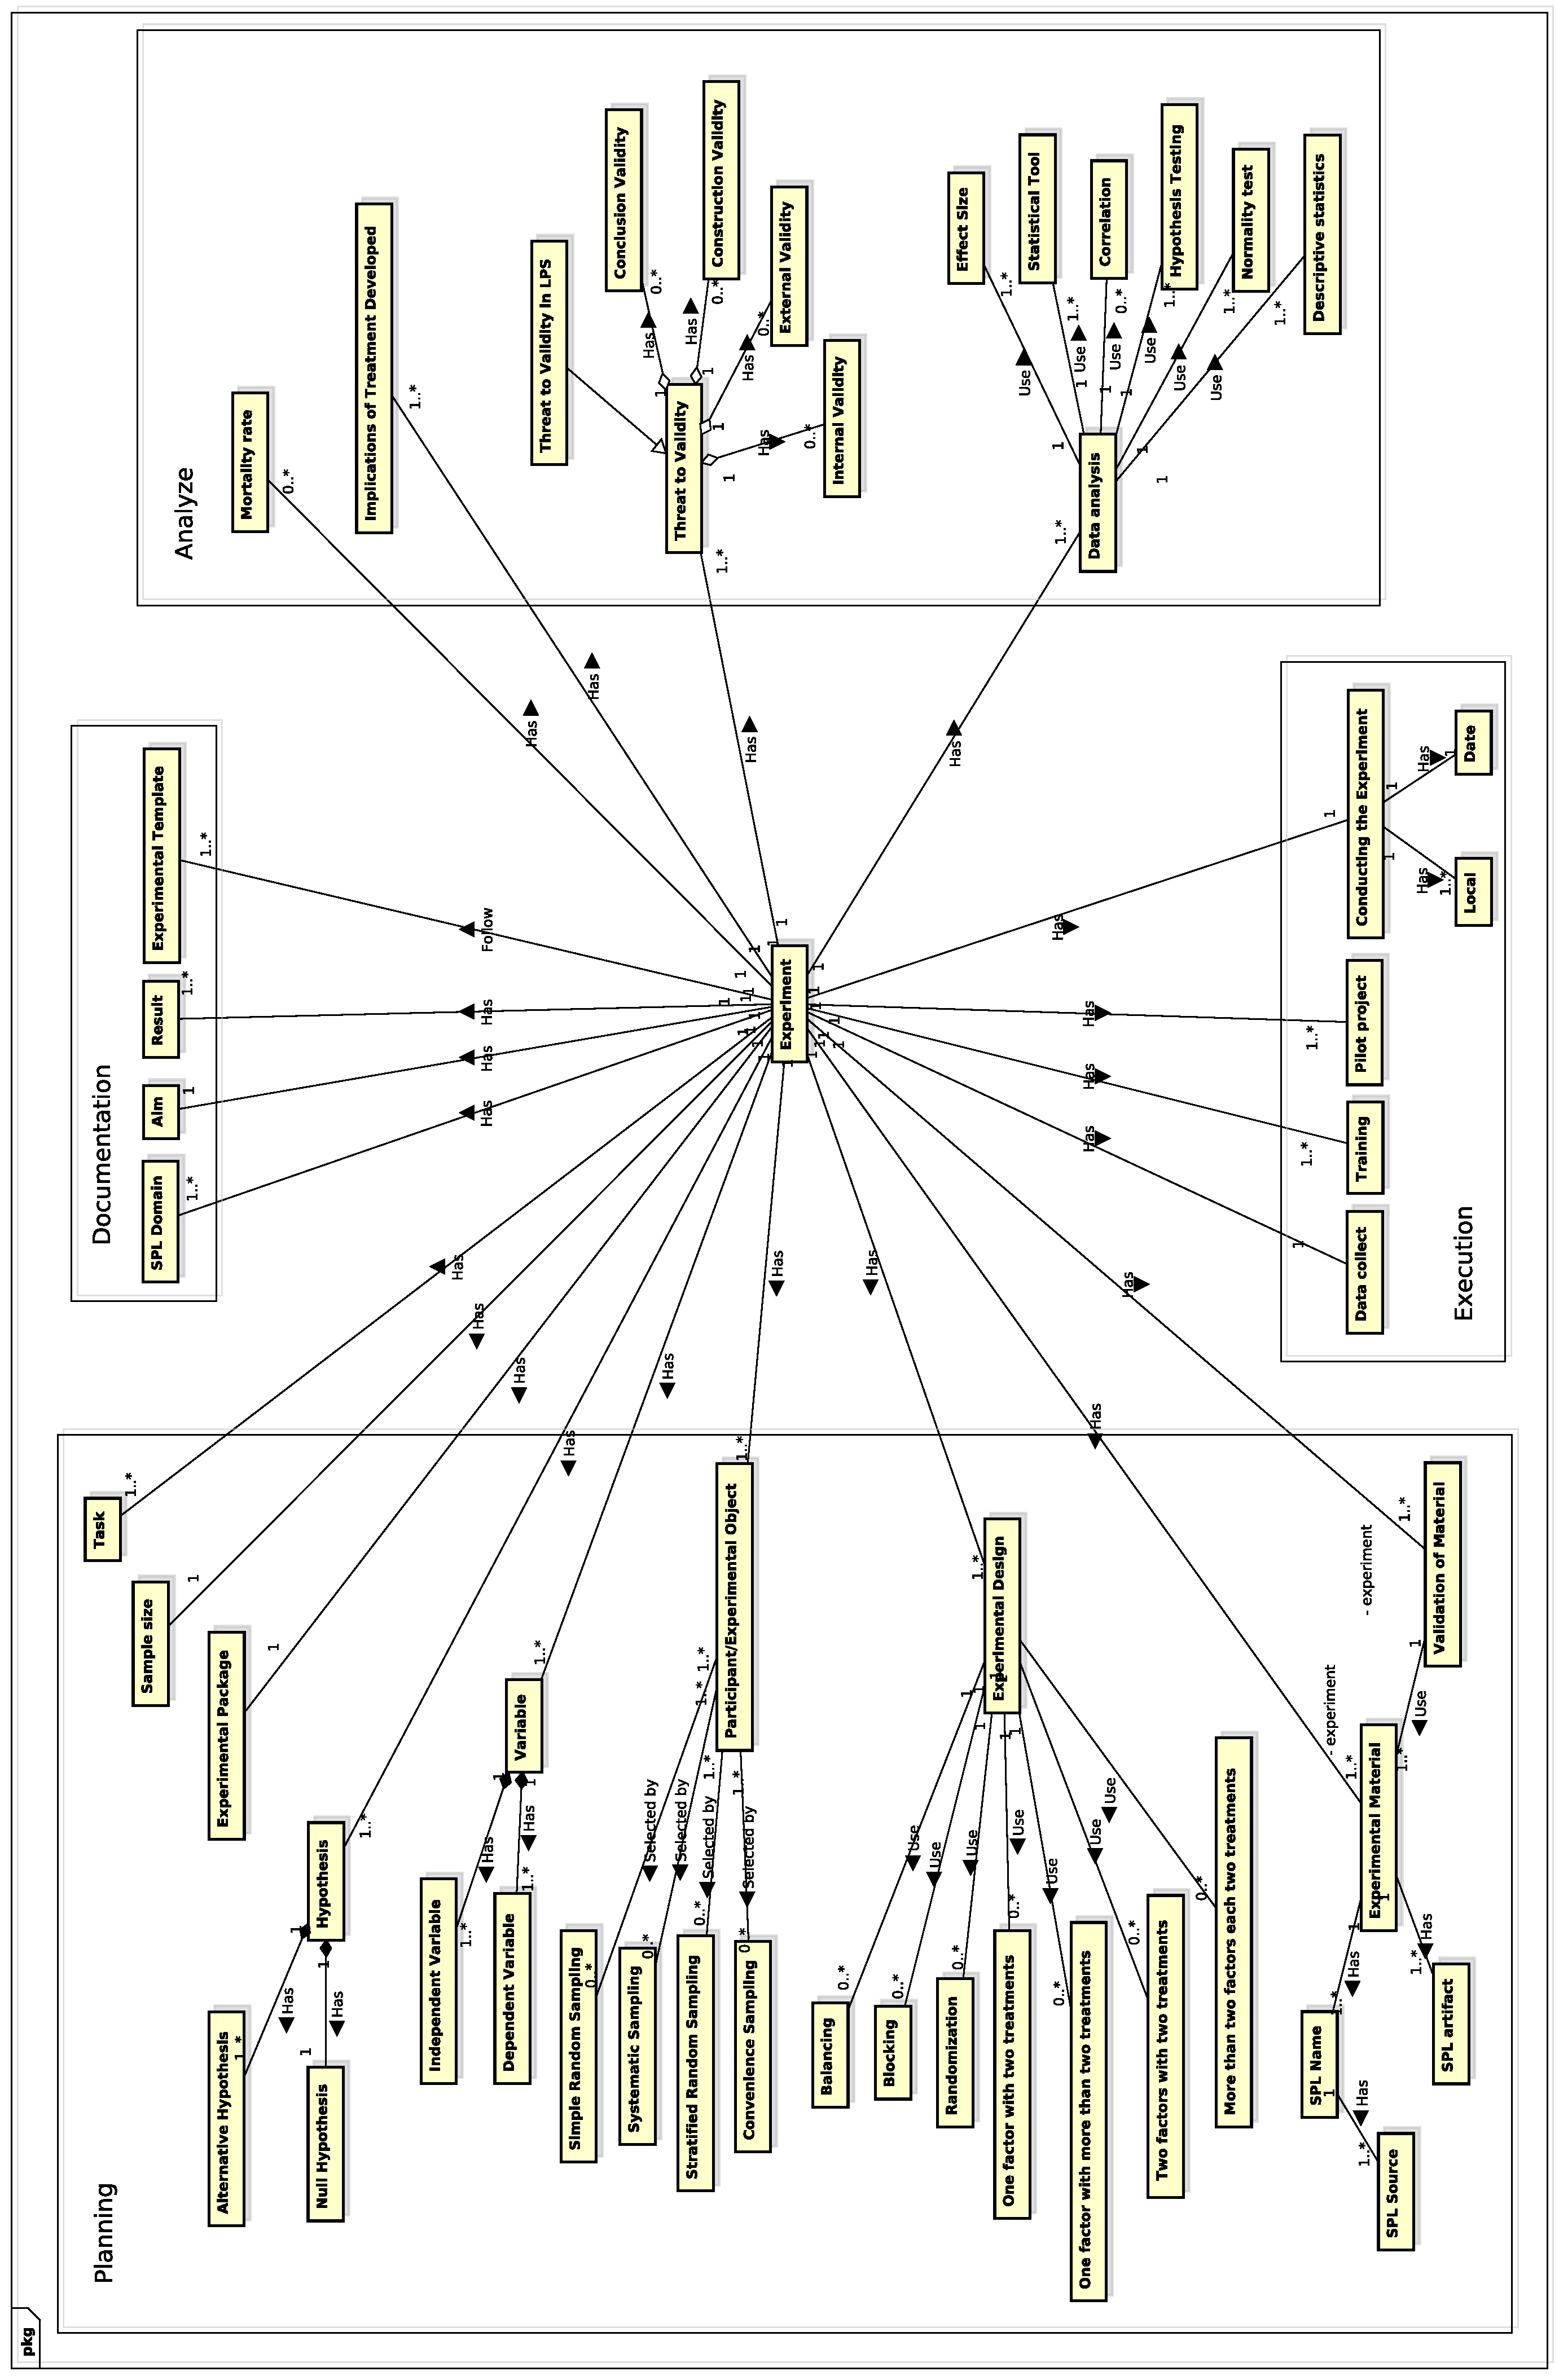
\includegraphics[scale=.2]{conceptual-model-clustering.pdf}
	\caption{Conceptual Model Clustering.}
	\label{figure:conceptual_model_clustering}
\end{figure}

A \ref{figure:conceptual_model_clustering}, apresenta uma modificação do modelo conceitual original, aplicando uma clusterização baseada nos pilares do Wohlin. Esta clusterização foi necessária para compreensão mais abstrata das relações entre os termos do domínio levantados no modelo conceitual original. Dessa forma foi possível validar as classes pai do grafo inicialmente proposto.
	
Em seguida, um diagrama de classes foi criado para uma representação mais formal da modelagem inicial. Nessa representação, a relação entre os termos (classes) e suas propriedades (atributos) ficou mais clara, o modelo TBox. Essa forma de representação destacou a relação principal quando definimos a composição da classe Experiment e ExperimentSPL em quase todas as outras subclasses. Nesta representação também foi explícita a tipificação das propriedades, modelo ABox.

\begin{figure}[htb]
	\centering
	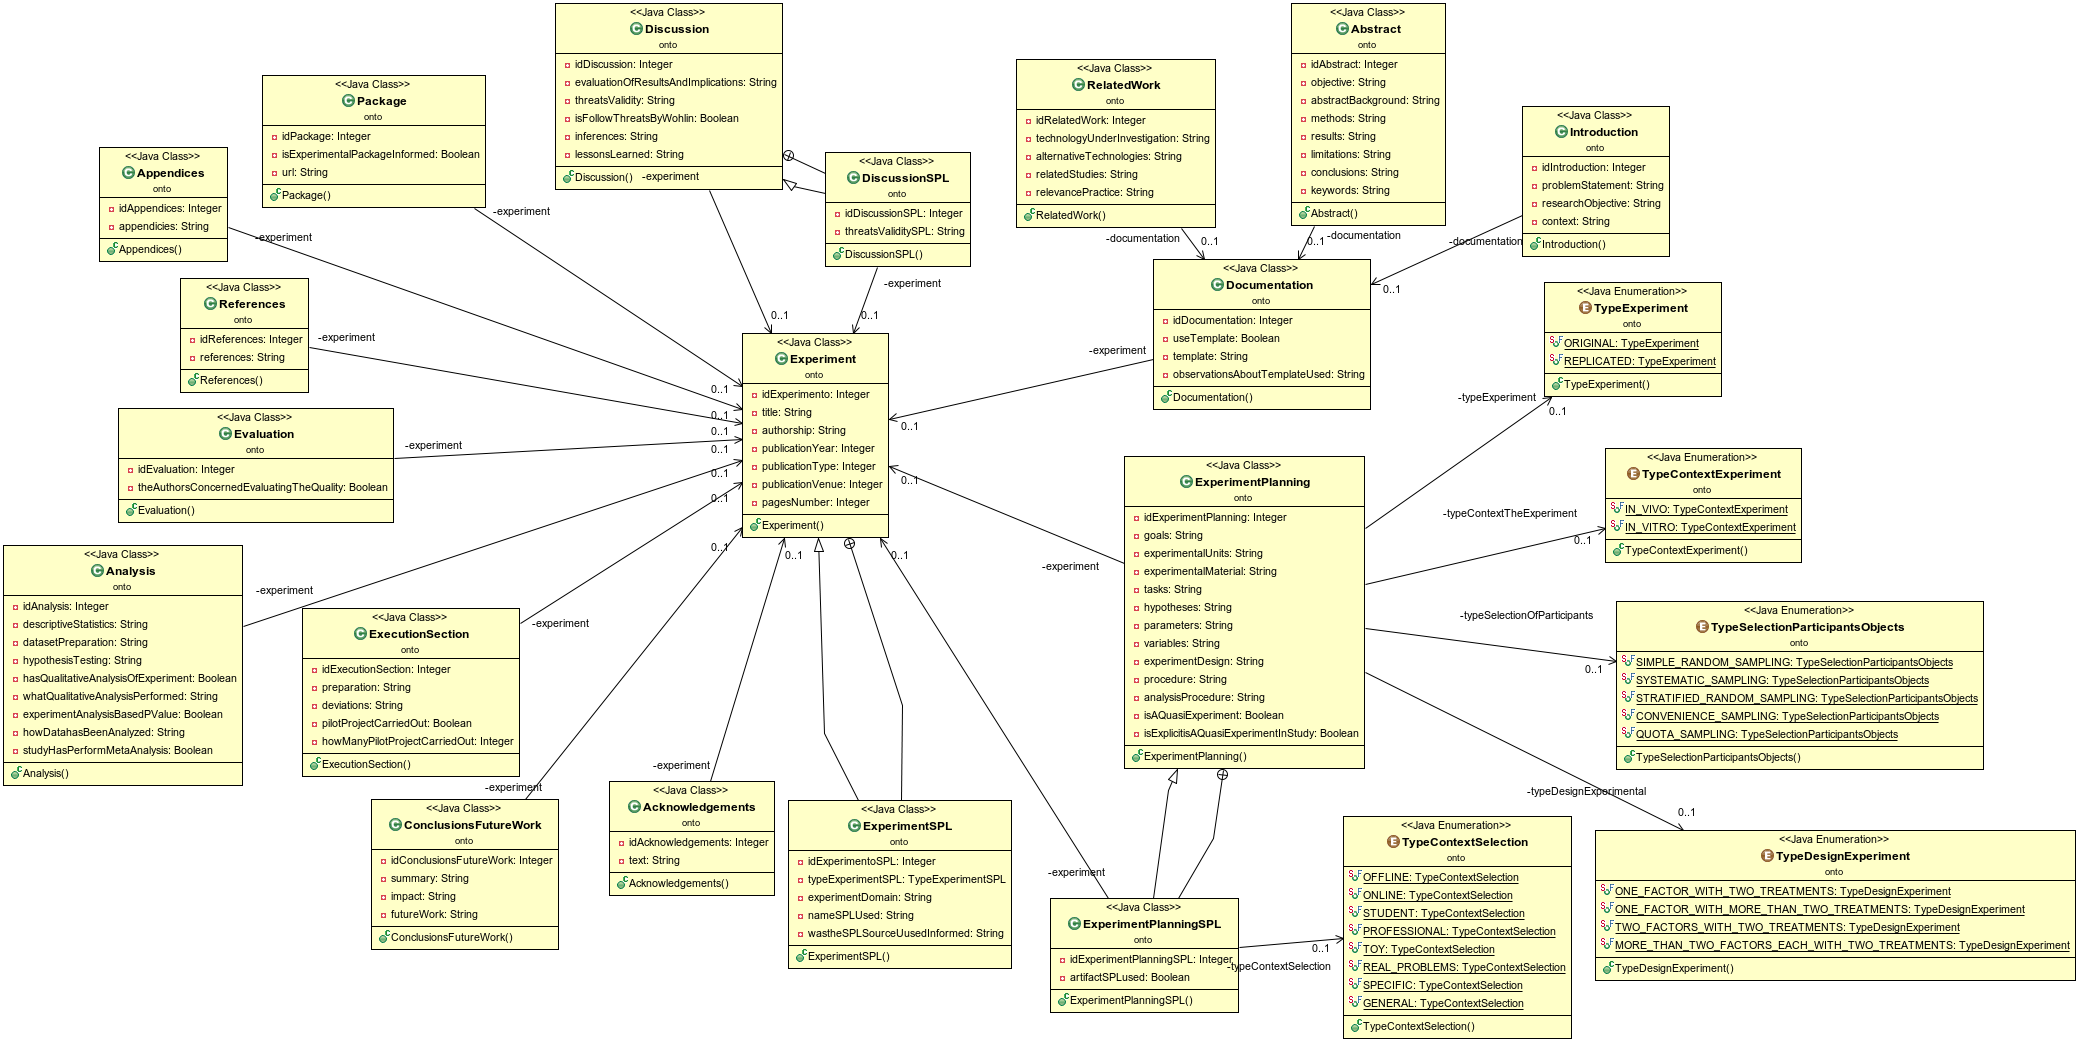
\includegraphics[scale=.2]{class-diagram-ontology.png}
	\caption{Class Diagram for proposal of the ontology model.}
	\label{figure:class_diagram_ontology}
\end{figure}

A \ref{figure:class_diagram_ontology} apresenta  diagrama de classe gerado para SMartyOntology.

Posteriormente, definimos usar a ferramenta Protégé para a construção oficial da ontologia. Esta ferramenta dispõe de uma interface gráfica para edição de ontologias e uma arquitetura para a criação de ferramentas baseadas em conhecimento. Pode ser usada tanto por desenvolvedores de sistema como por especialistas em domínio para criar bases de conhecimento, permitindo representar facilmente o conhecimento de uma área. Este editor é capaz de tratar classes, com sua definição e exemplos, simultaneamente \cite{DBLP:journals/aimatters/Musen15}.


\section{Projeto}
\label{sec:projeto}

Definimos a criação da ontologia usando OWL construindo as classes e subclasses para representar os elementos da ontologia.

\subsection{Protegé}
\label{sec:protege}

O padrão OWL foi usado no SMartyOntology para definir todos os elementos, classes e subclasses.

Fazendo uma analogia ao diagrama de classe, no Protégé, classes, os atributos de classes e seus relacionamentos estão em um contexto de entidades. As classes e hierarquias são definidos na aba Class, os relacionamentos são definidos na aba Propriedades de Objetos e os atributos são definidos na aba Propriedade dos Dados.

Definimos nossas entidades com base do diagrama de classe construído na fase de concepção, com a seguinte estrutura (i) definição de classes (ii) definição das propriedades de objetos, (iii) definição das propriedades dos dados.

\begin{table}[htbp]
	\caption{Ontology Design - Classes and Properties modeling}
	\label{tab:ontology_design_classes_properties}
	\centering
	\begin{tabu} to \textwidth {| p{1.4cm} | p{15.6cm} |}
		\hline
		\centering \textbf{Element} & \centering \textbf{Definition} \\ \hline
		
		Classes & Abstract, Acknowledgments, Analysis, Appendices, ConclusionsFutureWork, Discussion, DiscussionSPL, Documentation, Evaluation, ExecutionSection, Experiment, ExperimentSPL, ExperimentPlanning, ExperimentPlanningSPL, Introduction, Package, References, RelatatedWork, TypeContextExperiment, TypeContextSelection, TypeDesignExperiment, TypeEsperiment, TypeEsperimentSPL, TypeSelectioParticipantObjects \\ \hline
		
		Object Properties & documentation, experiment, typeContextxperiment, typeContextSelection, typeDesignExperiment, typeExperiment, typeExperimentSPL, typeSelectionOfParticipants \\ \hline
		
		Data \mbox{Properties} & idExperiment, title, authorship, publicationYear, publicationType, publicationVenue, pagesNumber, idExperimentSPL, nameSPLUsed, wasTheSPLSourceUsedInformed, idDocumentation, useTemplate, template, observationsAboutTemplateUsed, idAbstract, objective, abstractBackground, methods, results, limitations, conclusions, keywords, idIntroduction, problemStatement, researchObjective, context, idRelatedWork, technologyUnderInvestigation, alternativeTechnologies, relatedStudies, relevancePractice, idConclusionsFutureWork, summary, impact, futureWork, idExperimentPlanning, goals, experimentalUnits, experimentalMaterial, tasks, hypotheses, parameters, variables, experimentDesign, procedureProcedure, explicitQuesiExperimentInStudy, isAQuasiExperiment, idExperimentPlanningSPL, artifactSPLused, idExecutionSection, preparation, deviations, pilotProjectCarriedOut, howManyPilotProjectCarriedOut, idAnalysis, descriptiveStatistics, datasetPreparation, hyp othesisTesting, whatQualitativeAnalysisPerformed, howDatahasBeenAnalyzed, experimentAnalysisBasedPValue, hasQualitativeAnalysisOfExperiment, studyHasPerformMetaAnalysis, idDiscussion, evaluationOfResultsAndImplications, inferences, lessonsLearned, threatsValidity, isFollowThreatsByWohlin, idDiscussionSPL, threatsValiditySPL, idAcknowledgements, acknowledgments, idReferences, references, idAppendices, appendicies, idEvaluation, theAuthorsConcernedEvaluatingTheQuality, idPackage, isExperimentalPackageInformed, url, isLinkAvailable \\ \hline
	\end{tabu}
\end{table}

\subsubsection{Definição de classes}
No Protégé, definimos uma classe raiz chamada Thing na qual todas as outras classes são filhas dela. A \ref{figure:class_defition_protege} apresenta a definição da classe Experiment dentro do modelo, neste momento a definição é composta pelo nome da classe e seus principais relacionamentos (Equivalent To e SubClass Of).

\begin{figure}[]
	\centering 
	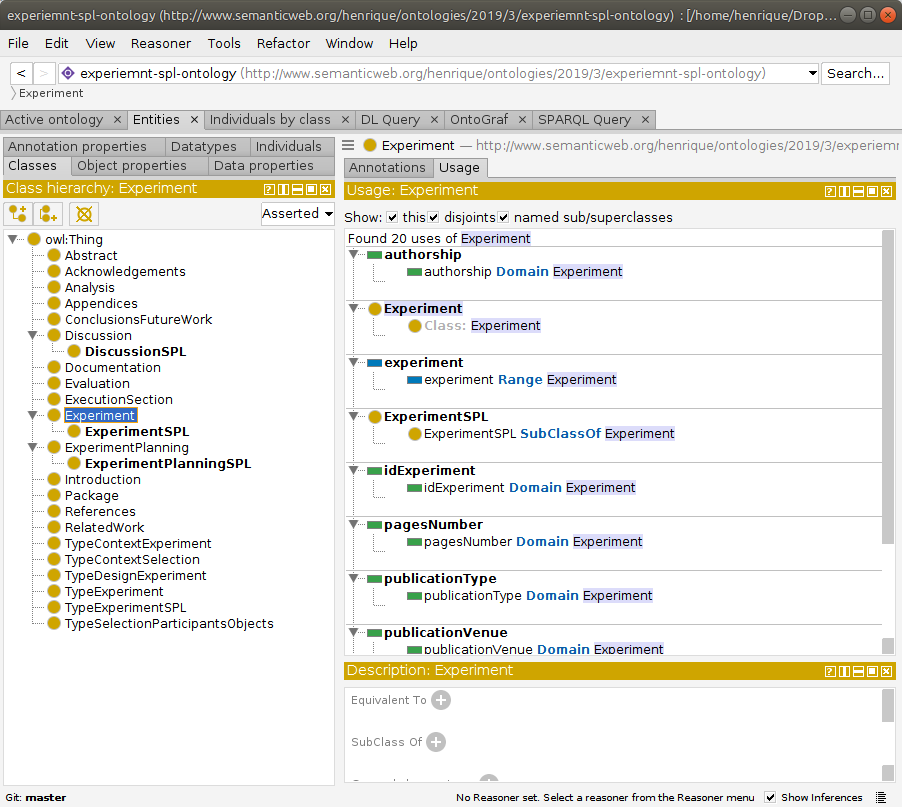
\includegraphics[scale=.3]{entidades-protege.png}
	\caption{Definição da classe Experiment no Protégé.}
	\label{figure:class_defition_protege}
\end{figure}

\subsubsection{Definição das propriedades de objetos}
No Protégé, definimos uma propriedade de objeto raiz chamada topObjectProperty na qual todas as outras propriedades são filhas dela. A \ref{figure:object_prop_defition_protege} Figura apresenta a definição de propriedade de objeto para chamada ?documentation? dentro do modelo, neste momento a definição é composta pelo nome da propriedade e seus relacionamentos com classes, Domains e Ranges.

\begin{figure}[htb]
	\centering 
	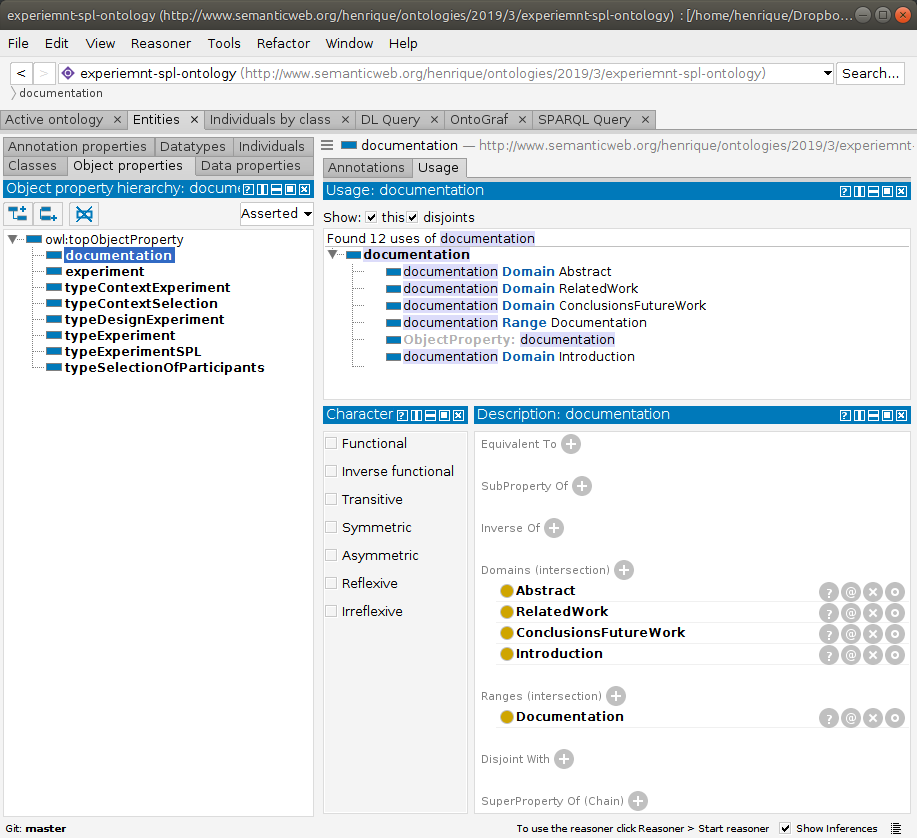
\includegraphics[width=10cm]{entidades-protege-object-properties.png}
	\caption{Definição da propriedade de objeto documentation no Protégé.}
	\label{figure:object_prop_defition_protege}
\end{figure}

\subsubsection{Definição das propriedades dos dados}
No Protégé, definimos uma propriedade de dados raiz chamada topDataProperty na qual todas as outras propriedades são filhas dela. Para cada Propriedade de Dado definimos um conjunto de classes de seu Domínio e um conjunto de tipos de dados (predefinido) de seu Alcance, por exemplo, a propriedade de dado ?nameSPLUsed? possui como classe de domínio ExperimentSPL e como alcance um xsd:string. A \ref{figure:data_prop_defition_protege} apresenta a definição de propriedade de dado para chamada ?nameSPLUsed? dentro do modelo, neste momento a definição é composta pelo nome da propriedade e seus relacionamentos, Domains (uma classe) e Ranges (uma tipagem).

\begin{figure}[htb]
	\centering 
	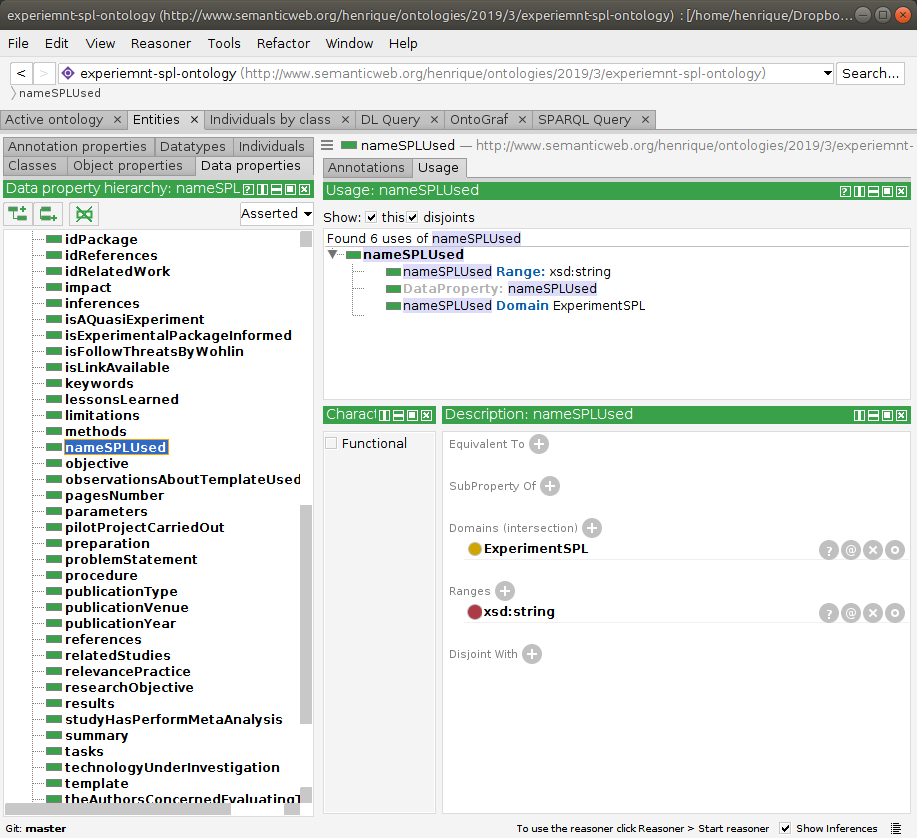
\includegraphics[width=10cm]{entidades-protege-data-properties.png}
	\caption{Definição da propriedade de dado nameSPLUsed no Protégé.}
	\label{figure:data_prop_defition_protege}
\end{figure}

\subsubsection{Artefato gerado pelo Protégé}

Ao final, o Protégé gera um arquivo .owl contendo a definição do modelo. A \ref{figure:graph_ontology_model} fornece uma visão geral do formato do grafo do projeto, contendo todas as classes e suas propriedades de objeto e propriedade de dados. Usamos a ferramenta WebVOWL \cite{lohmann2016visualizing} para gerar essa visão.

\begin{figure}[htb]
	\centering 
	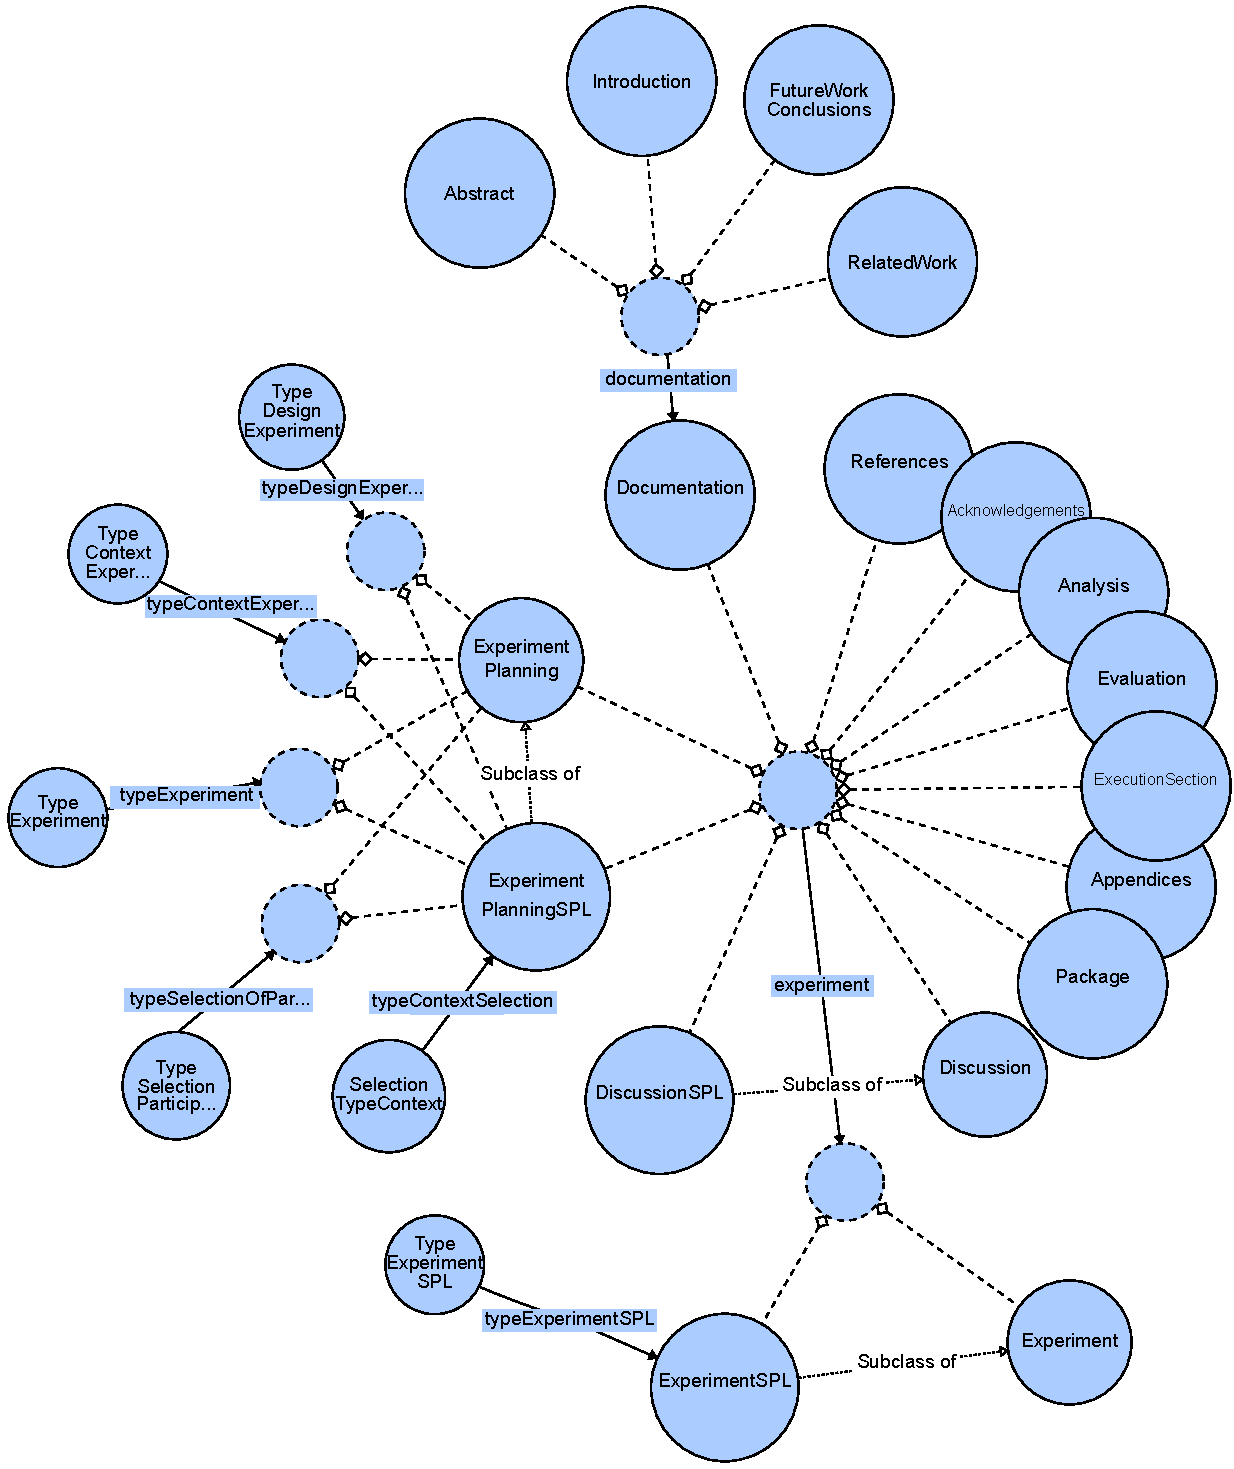
\includegraphics[width=10cm]{ontology-populate-valid-owl-2.pdf}
	\caption{Grafo da modelagem da ontologia - gerado pelo WbVOWL.}
	\label{figure:graph_ontology_model}
\end{figure}

\subsection{Pyton}
\label{sec:python}

A próxima etapa, após a modelagem da ontologia, foi inserir os indivíduos na mesma, ou seja, popular a ontologia para realização de inferências futuras. Apesar do Protégé ter capacidade para realizar essa operação, optamos por utilizar um script para realizar tal tarefa, visto que, no Protégé o processo de inserir indivíduos na ontologia é realizado de modo manual, por meio do menu ?Individuals by Class?, onde é preciso selecionar propriedade por propriedade para cada indivíduo. Sabendo que para cada indivíduo temos 84 propriedades de dados mais 8 propriedade de objetos, somando um total de 92 relacionamentos para cada indivíduo. Portanto, sabendo que temos 174 indivíduos a serem inseridos em uma carga inicial, seriam mais de 16000 iterações manuais no Protégé.

Dado essa estimativa de operações manuais optamos pela utilização de uma ferramenta script a fim de facilitar e automatizar a inserção dos indivíduos e posteriormente a inserção de novos indivíduos. Escolhemos a linguagem de programação Python por fornecer bibliotecas prontas, tanto para manipulação de dados em planilhas (Pandas), como para ontologia em arquivos .owl (OwlReady2).

\subsubsection{Script}

Para criação do script utilizamos outra ferramenta do Python chamada Jupyter Notebook \cite{PER-GRA:2007} para auxiliar na execução e validação de código. O processo do script se assemelha a um processo de ETL (Extract Transform Load), onde extraímos os dados originais da planilha, desenvolvida no trabalho de revisão sistemática sobre experimentos em LPS, e manipulamos estes dados para inserir na ontologia, seguindo a modelagem inicial construída no Protégé.

Para  leitura dos dados da planilha usamos a biblioteca Pandas \cite{mckinney-proc-scipy-2010}, ela nos retorna um objeto do tipo Dataframe que chamamos de ?df?, no qual é a representação da própria planilha no ambiente de programação Python.

Os dados da planilha estão estruturados na seguinte forma, cada linha representa um artigo encontrado no mapeamento sistemático, e cada coluna representa um dado extraído deste artigo. Segue o mapeamento de cada dado. 

Com relação ao Experimento temos:  ID,  Title, Authorship, Publication year, Publication type, Publication venue, Pages number, dados de Experimentos em SPL temos: Is it Real or Academic SPL?, SPL Name used, Was the SPL source used informed? (Y/N) (If yes, which one?). 

Com relação a Documentation temos: Does it use template? (Y/N)?,  If yes, what template?, Observations about the template used. Para o Abstract temos: Objective (What is the question addressed with this research?), Abstract - Background (Why is this research important?), Methods (What is the statistical context and methods applied?), Results (What are the main findings? Practical implications?), Limitations (What are the weakness of this research?), Conclusions (What is the conclusion?) e Keywords. Para o Introduction Section temos: Problem statement (What is the problem? Where does it occur? Who has observed it? Why is it important to be solved?), Research objective (GQM) (What is the research question to be answered by this study?), Context (What information is necessary to understand whether the research relates to a specific situation (environment)?). Para o Related Work Section temos: Technology under investigation (What is necessary for a reader to know about the tecnology to reproduce its application?), Alternative technologies (How does this research relate to alternative technologies? What is the control treatment?), Related studies (How this research relates to existing research (studies)? What were the results from these studies?), Relevance to practice (How does it relate to state of the practice?). Para o Conclusions and Future Work Section temos: Summary (The purpose of this section is to provide a concise summary of the research and its results as presented in the former sections), Impact (Description of impacts with regard to cost, schedule, and quality, circumstances under which the approarch presumably will not yield the expected benefit), Future Work (What other experiments could be run to further investigate the results yielded or evolve the Body of Knowledge).

Com relação ao Experiment Planning temos: Goals (Formalization of goals, refine the important constructs of the experiment's goal), Experimental Units (From which population will the sample be drawn? How will the groups be formed (assignment to treatments)? Any kind of randomization and blinding has to be described?), Experimental Material (Which objects are selected and why?), Tasks (Which tasks have to be performed by the subjects?), Hypotheses (What are the constructs and their operationalization? They have to be traceable derived from the research question respectively the goal of the experiment), Parameters (What are the constructs and their operationalization? They have to be traceable derived from the research question respectively the goal of the experiment), Variables (What are the constructs and their operationalization? They have to be traceable derived from the research question respectively the goal of the experiment), Experiment Design (What type of expimental design has been chosen?), Procedure (How will the experiment (i.e., data collection) be performed? What instruments, materials, tools will be used and how?) Analysis Procedure (How will the data be analyzed?), Is it a quasi-experiment? (Y/N) If yes, is it explicit in the study?, Is it an Original or Replicated Experiment?,	How was the selection of participants/experimental objects? - Simple random sampling; - Systematic sampling; - Stratified random sampling; - Convenience sampling; - Quota sampling, Context of the experiment (in vivo, in vitro, ...), Design Experimental: - One factor with two treatments; - One factor with more than two treatments; - Two factors with two treatments; - More than two factors each with two treatments, SPL artifact used, Context Selection (Off-line vs. on-line, Student vs. professional, Toy vs. real problems, Specific vs. general).

Com relação a Execution (Operation) temos: Preparation (What has been done to prepare the execution of the experiment (i.e., schedule, training), Deviations from the Plan (Describe any deviations from the plan, e.g., how was the data collection actually performed?), The pilot project was carried out? (Y/N) If Yes, how many?

Com relação a Analysis (Analysis and Interpretation) temos: Descriptive statistics (What are the results from descriptive statistics?), Data set preparation (What was done to prepare the data set, why, and how?), Hypothesis testing (How was the data evaluated and was the analysis model validated?), Do it have qualitative analysis of the experiment? (Y/N), If yes, what qualitative analysis was performed?, How the data has been analyzed? (Ex: Correlation, Hypothesis Test, meta-analysis), Is the conclusion of the experiment analysis based on P-value? (Y/N), Did the study perform meta-analysis? (Y/N).

Com relação a Discussion temos: Evaluation of Results and Implications (Explain the results and the relation of the results to earlier research, especially those mentioned in the Background section), Threats to Validity (How is validity of the experimental results assured? How was the data actually validated?) (Follow are the 4 threats proposed by Wohlin: internal, external, construct and conclusion? (Y/N)), Inferences (Inferences drawn from the data to more general conditions), Lessons learned (Which experience was collected during the course of the experiment), Threats to validity in SPL.

Com relação a Evaluation temos: The authors were concerned with evaluating the quality of the experiments? (Y/N)

Com relação a Package temos: Is the experimental package informed? (Y/N) (If yes, what URL? And the link is still available? (Y/N))

Outros dados: Acknowledgements Section (Sponsors, participants, and contributors who do not fullfit the requirements for authorship should be mentioned), References Section (All cited literature has to be presented in the format requested by the publisher, Appendices Section (Experimental materials, raw data, and detailed analyses, which might be helpful for others to build upon the reported work should be provided)

\subsubsection{Manipulação dos Dados}

Para inserir os indivíduos na SMartyOntology, foi preciso manipular os dados da planilha com as seguintes operações.

Primeira operação, split de dados de uma única coluna para duas propriedades de dados da ontologia. Este caso ocorreu para os seguintes dados, as propriedades e prefixadas com ?\_? foram tratadas no próximo passo:

\begin{itemize}
	\item ?Was the SPL source used informed? (Y/N) (If yes, which one?)? para \_informedSPL e sourceSPL;
	\item ?The pilot project was carried out? (Y/N) If Yes, how many?? para \_hasPilot e \_howManyPilot;
	\item ?Is it a quasi-experiment? (Y/N) If yes, is it explicit in the study?? para \_hasQuasiExperiment e quasiExperiment;
	\item ?'Threats to Validity (How is validity of the experimental results assured? 'How was the data actually validated?) (Follow are the 4 threats proposed by Wohlin: internal, external, construct and conclusion? (Y/N)))? para \_hasThreatsValidityByWolin e threatsValidity.
\end{itemize}

Segunda operação, transformação de dados booleanos, strings vazias e números. Foi desenvolvido tres funções de conversão, (i) convertToBoolean, (ii) convertStringEmpty e (iii) convertToNumber. Este caso ocorreu para os seguintes dados:

\begin{itemize}
	\item ?Does it use template? (Y/N)?? para useTemplate aplicando o método convertToBoolean;
	\item ?If yes, what template?? para template aplicando o método convertStringEmpty;
	\item ?Do it have qualitative analysis of the experiment? (Y/N)? para hasQualitativeAnalysis aplicando o método convertToBoolean;
	\item ?Did the study perform meta-analysis? (Y/N)? para hasMetaAnalysis aplicando o método convertToBoolean;
	\item \_informedSPL para informedSPL aplicando o método convertToBoolean;
	\item \_hasQuasiExperiment para hasAQuasiExperiment aplicando o método convertToBoolean;
	\item \_hasPilot para hasPilot aplicando o método convertToBoolean;
	\item \_howManyPilot para howManyPilot aplicando o método convertToNumber;
	\item \_hasThreatsValidityByWolin para hasThreatsValidityByWolin aplicando o método convertToBoolean;
	\item \_hasPackage para hasExperimentalPackage aplicando o método convertToBoolean;
\end{itemize}

Terceira operação, separação do conjunto de dados com informação explícita de SPL. Separamos o conjunto total de 174 artigos em artigos de experimentos que contêm informações explícitas de SPL (152) e artigos que não contêm informação explícitas de SPL (22), para criação dos indivíduos conforme as classes modeladas na ontologia com atributos pertinentes a SPL.

Quarta operação, padronização de dados constantes e faltantes. Foi preciso padronizar os dados em casos faltantes foi atribuído um padrão. Isso ocorreu para os seguintes dados:

\begin{itemize}
	\item "Is it Real or Academic SPL?" foi definido o seguinte conjunto de dados [REAL, ACADEMY] sendo o padrão "ACADEMY";
	\item "Is it an Original or Replicated Experiment?" foi definido o seguinte conjunto de dados [ORIGINAL, REPLICATED] sendo o padrão "REPLICATED"
	\item "How was the selection of participants/experimental objects? - Simple random sampling; - Systematic sampling; - Stratified random sampling; - Convenience sampling; - Quota sampling." foi definido o seguinte conjunto de dados [SIMPLE\_RANDOM\_SAMPLING, SYSTEMATIC\_SAMPLING, STRATIFIED\_RANDOM\_SAMPLING,	CONVENIENCE\_SAMPLING, QUOTA\_SAMPLING] sendo o padrão "CONVENIENCE\_SAMPLING";
	\item "Context of the experiment (in vivo, in vitro, ...)" foi definido o seguinte conjunto de dados [IN\_VIVO, IN\_VITRO] sendo o padrão "IN\_VITRO";
	\item "Design Experimental: - One factor with two treatments; - One factor with more than two treatments; - Two factors with two treatments; - More than two factors each with two treatments." foi definido o seguinte conjunto de dados [ONE\_FACTOR\_WITH\_TWO\_TREATMENTS, ONE\_FACTOR\_WITH\_MORE\_THAN\_TWO\_TREATMENTS, TWO\_FACTORS\_WITH\_TWO\_TREATMENTS, MORE\_THAN\_TWO\_FACTORS\_EACH\_WITH\_TWO\_TREATMENTS] sendo o padrão "ONE\_FACTOR\_WITH\_TWO\_TREATMENTS";
	\item "Context Selection (Off-line vs. on-line, Student vs. professional, Toy vs. real problems, Specific vs. general)" foi definido o seguinte conjunto de dados [OFFLINE, ONLINE, STUDENT, PROFESSIONAL, TOY, REAL\_PROBLEMS, SPECIFIC, GENERAL] sendoo padrão "GENERAL";
\end{itemize}

\subsubsection{Inserção do indivíduos e criação dos relacionamentos}

Inicialmente fazemos a leitura do modelo da ontologia gerada pelo Protégé (arquivo .owl) por meio da biblioteca Owlready2, com isso temos um objeto chamado ?onto? onde a partir dele podemos executar operações de inserção de indivíduos e outras operações na ontologia no ambiente de programação Python.

O processo de inserção dos dados extraídos da planilha se dá por, percorrer linha a linha da planilha, e criar os indivíduos um a um de cada classe modelada na ontologia com seus respectivos atributos. Para isso foi necessário criar vários métodos a fim de facilitar a compreensão do script.

Foi criado dois laços para percorre os dois subconjuntos de dados, um com informações explícitas de SPL chamado de df\_spl  e outro chamado df\_exp. O primeiro laço sobre df\_spl invoca a seguinte sequencia de métodos: registreExperimentSPL > registreExperimentPlanningSPL > registreDiscussionSPL > registerCommons. O segundo laço sobre df\_exp invoca a seguinte sequencia de métodos: registreExperiment > registreExperimentPlanning > registreDiscussion > registerCommons.

\begin{lstlisting}[language=Python, caption=The first loop on \texttt{df\_spl}, label=lst:first-loop]
for idx, row in df_spl.iterrows():
experimentSPL = registreExperimentSPL(idx, row)

experimentPlanningSPL = registreExperimentPlanningSPL(idx, row)
experimentPlanningSPL.experiment.append(experimentSPL)

discussion = registreDiscussionSPL(idx, row)
discussion.experiment.append(experimentSPL)

registerCommons(experimentSPL, idx, row)
\end{lstlisting}

\begin{lstlisting}[language=Python, caption=The second loop on \texttt{df\_exp}, label=lst:second-loop]
for idx, row in df_exp.iterrows():
experiment = registreExperiment(idx, row)

experimentPlanning = registreExperimentPlanning(idx, row)
experimentPlanning.experiment.append(experiment)

discussion = registreDiscussion(idx, row)
discussion.experiment.append(experiment)

registerCommons(experiment, idx, row)
\end{lstlisting}

O método registreExperimentSPL executa o método registreExperimentCommons e retorna uma instância de indivíduo da ontologia da classe onto.ExperimentSPL.

O método registreExperiment executa o método registreExperimentCommons e retorna uma instância de indivíduo da ontologia da classe onto.Experiment.

O método registreExperimentCommons recebe uma instância tanto de onto.ExperimentSPL ou onto.Experiment e atribui as variáveis comuns para ambas as classes.

O método registreExperimentPlanningSPL executa o método registreExperimentPlanningCommons e retorna uma instância de indivíduo da ontologia da classe onto.ExperimentPlanningSPL.

O método registreExperimentPlanning executa o método registreExperimentPlanningCommons e retorna uma instância de indivíduo da ontologia da classe onto.ExperimentPlanning.

O método registreExperimentPlanningCommons recebe uma instância tanto de onto.ExperimentPlanningSPL ou onto.ExperimentPlanning e atribui as variáveis comuns para ambas as classes.

O método registreDiscussionSPL executa o método registreDiscussionCommons e retorna uma instância de indivíduo da ontologia da classe onto.DiscussionSPL.

O método registreDiscussion executa o método registreDiscussionCommons e retorna uma instância de indivíduo da ontologia da classe onto.Discussion.

O método registreDiscussionCommons recebe uma instância tanto de onto.DiscussionSPL ou onto.Discussion e atribui as variáveis comuns para ambas as classes.

O método registerCommons que recebe uma instância tanto de onto.ExperimentSPL ou onto.Experiment e executa a sequência de métodos:  registreDocumentation - que retorna uma instância de onto.Documentation e atribui a instância de experiment a ela > registreAbstract - que retorna uma instância de onto.Abstract e atribui a instância de documentation a ela > registreIntroduction - que retorna uma instância de onto.Introduction e atribui a instância de documentation a ela > registreRelatedWork - que retorna uma instância de onto.RelatedWork e atribui a instância de documentation a ela > registreConclusionsFutureWork - que retorna uma instância de onto.ConclusionsFutureWork e atribui a instância de documentation a ela > registreExecutionSection - que retorna uma instância de onto.ExecutionSection e atribui a instância de experiment a ela > registreAnalysis - que retorna uma instância de onto.Analysis e atribui a instância de experiment a ela > registreAcknowledgements - que retorna uma instância de onto.Acknowledgements e atribui a instância de experiment a ela > registreReferences - que retorna uma instância de onto.References e atribui a instância de experiment a ela > registreAppendices - que retorna uma instância de onto.Appendices e atribui a instância de experiment a ela > registreEvaluation - que retorna uma instância de onto.Evaluation e atribui a instância de experiment a ela > registrePackage - que retorna uma instância de onto.Package e atribui a instância de experiment a ela.

\subsubsection{Artefato e validação}
Ao final dos dois laços temos o objeto ?onto? populado com com os indivíduos, e por meio da biblioteca Owlready2 geramos um novo arquivo .owl contendo a modelagem da ontologia mais a população de indivíduos. O arquivo da modelagem inicial contém 66,3 kB, e o arquivo populado contém 4,8 MB.

No final do script tem existe um passo de validação onde conferimos a quantidade de linhas da planilha com a quantidade de indivíduos inserido na ontologia, pode ser visto em \ref{lst:stap-validation}.

\begin{lstlisting}[language=Python, caption=Stap validation, label=lst:stap-validation]
assert len (onto.Experiment.instances ()) == df.shape [0]
\end{lstlisting}

\section{Exemplo de Aplicação}
\label{sec:exemplo}

Foi criado também um exemplo de recomendação com a seguinte questão de recomendação, ?Qual artefato de SPL usar dos experimentos que usam a mesma template experimental mais recorrente?. Com base nesta questão foi criado um script Python utilizando as bibliotecas Pandas e OwlReady2, para responder a mesma.

O script começa carregando a ontologia preenchida e, em seguida, executamos a consulta SPARQL \ref{code:...} para retornar os agrupados pela template experimental, estes indivíduos são do tipo Documentation. Na sequência, filtramos da lista inicial de indivíduos que usam modelos, aqueles que usam o modelo mais recorrente. Com esses indivíduos em mãos, buscamos seu relacionamento com indivíduos do tipo ExperimentPlanningSPL para extrair informações de artefatos de SPL. Assim, podemos recomendar qual artefato de SPL, com base no artefato mais usado desses indivíduos filtrados.

O script começa carregando a ontologia povoada, e em seguida extrai os indivíduos que usam template experimental, estes indivíduos são do tipo Documentation. Atribuímos este resultado a um objeto do tipo Pandas para executar a função .values\_counts() que retorna o agrupamento somado das templates mais usadas. Na sequência, filtramos da lista inicial dos indivíduos que usam templates, aqueles que usam a template mais recorrente. Com estes indivíduos em mãos, buscamos o relacionamento deles com os indivíduos do tipo ExperimentPlanningSPL para extrair a informação dos artefatos de SPL. Então podemos recomendar qual artefato de SPL, com base no artefato mais usado destes individuos filtrados.

\begin{figure}[ht]
 	\centering 
 	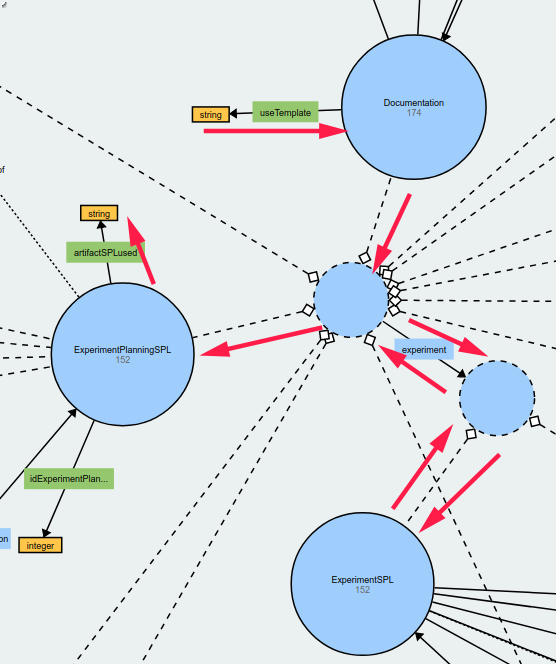
\includegraphics[width=6.5cm]{filter-in-ontology-path.png}
 	\caption{Graph Path to Recommendation Example.}
 	\label{figure:graph_path_to_recomendation}
 \end{figure}

O grafo da \ref{figure:graph_path_to_recomendation} mostra o caminho percorrido entre as classes e propriedades de objetos e dados para chegar no artefato de SPL a ser recomendado.

O exemplo de recomendação apresenta como podemos criar mecanismos de inferência no modelo de ontologia proposto neste trabalho. Foi possível avaliar que com algumas consultas e verificações é possível extrair informações e meta informações sobre experimentos em SPL. 

Este exemplo percorre três classes (Documentation, ExperimentSPL e ExperimentPlanningSPL) de 24 classes, duas propriedades de objetos (documentation e experimet) de 8 propriedades e três propriedades de dados (useTemplate, template e artifactSPLused) de 87 propriedades de dados do modelo proposto. O cálculo . estima que neste exemplo estamos usando 0,1% da capacidade de resposta que o modelo possa responder.

%uso de classe * %uso de propriedade de objeto * %uso de propriedade de dados = %uso da ontologia.

O exemplo apresenta como podemos criar mecanismos de inferência no modelo de ontologia proposto neste trabalho. Foi possível avaliar que com algumas consultas e verificações é possível extrair informações e meta informações sobre experimentos em SPL. 

Este exemplo percorre três classes (Documentation, ExperimentSPL e ExperimentPlanningSPL) de 24 classes, duas propriedades de objetos (documentation e experimet) de 8 propriedades e três propriedades de dados (useTemplate, template e artifactSPLused) de 87 propriedades de dados do modelo proposto. O cálculo . estima que neste exemplo estamos usando 0,1\% da capacidade de resposta que o modelo possa responder.

%uso de classe * %uso de propriedade de objeto * %uso de propriedade de dados = %uso da ontologia.

%****CÁLCULO DO USO ESTIMADO DA ONTOLOGIA*** POSSIBILIDADES DE CAMINHOS ENTRE CLASSES E PROPRIEDADES.

No caso do exemplo de recomendação a primeira parte do retorna a template mais recorrente. O resultado é a saída do script: ?Template more frequency is Wohlin? seguida da Fig. que representa os dados da Tabela.

E segunda parte encontra qual artefato de SPL dos indivíduos que usam a template encontrada na primeira etapa. o resultado é a saída do script: ?Artifact more used is the "test cases" to template: Wohlin? seguido da Fig.

\section{Avaliação Empírica}
\label{sec:avaliacao}

Para avaliação da ontologia seguimos duas estratégias, uma para avaliar possíveis armadilhas e falhas no modelo de ontologia proposto.

Usamos a ferramenta OOPS! para gerar avaliação do modelo de ontologia proposto. A ferramenta ajuda a detectar algumas das armadilhas mais comuns que aparecem ao desenvolver ontologias [referência].

\begin{itemize}
	\item P01. Criando elementos polissêmicos;
	\item P02. Criando sinônimos como classes;
	\item P03. Criando o relacionamento `` is '' em vez de usar `` rdfs: subClassOf ''; `` rdf: type '' ou `` owl: sameAs '';
	\item P04. Criando elementos de ontologia não conectados;
	\item P05. Definindo relações inversas erradas;
	\item P06. Incluindo ciclos em uma hierarquia de classes;
	\item P07. Mesclar diferentes conceitos na mesma classe;
	\item P08. Anotações ausentes;
	\item P09. Informações de domínio ausentes;
	\item P10. Desarticulação em falta;
	\item P11. Domínio ou intervalo ausente nas propriedades;
	\item P12. Propriedades equivalentes não explicitamente declaradas;
	\item P13. Relações inversas não explicitamente declaradas;
	\item P14. Uso indevido de `` owl: allValuesFrom '';
	\item P15. Usando `` alguns não '' no lugar de `` não alguns '';
	\item P16. Usando uma classe primitiva no lugar de uma definida;
	\item P17. Superespecialização de uma hierarquia;
	\item P18. Superespecialização do domínio ou intervalo;
	\item P19. Definir vários domínios ou intervalos nas propriedades;
	\item P20. Uso indevido de anotações de ontologia;
	\item P21. Usando uma classe diversa;
	\item P22. Usando diferentes convenções de nomenclatura na ontologia;
	\item P23. Duplicando um tipo de dados já fornecido pela linguagem de implementação;
	\item P24. Usando definições recursivas;
	\item P25. Definir um relacionamento como inverso de si mesmo;
	\item P26. Definindo relações inversas para uma simétrica;
	\item P27. Definir propriedades equivalentes erradas;
	\item P28. Definindo relacionamentos simétricos errados;
	\item P29. Definindo relacionamentos transitivos errados;
	\item P30. Classes equivalentes não explicitamente declaradas;
	\item P31. Definir classes equivalentes erradas;
	\item P32. Várias aulas com o mesmo rótulo;
	\item P33. Criando uma cadeia de propriedades com apenas uma propriedade;
	\item P34. Classe sem tipografia;
	\item P35. Propriedade não tipificada;
	\item P36. URI contém extensão de arquivo;
	\item P37. Ontologia não disponível na Web;
	\item P38. Nenhuma declaração de ontologia OWL;
	\item P39. Namespace ambíguo;
	\item P40. Sequestro de namespace;
	\item P41. Nenhuma licença declarada.
\end{itemize}

Apesar da ferramenta OOPS! ter 41 pontos de avaliação ela executa apenas 34 pontos semi-automaticamente, pois os outros dependem de domínio específico da ontologia e eles encorajam os usuários a melhorarem a ferramenta. O resultado dado pela ferramenta sugere como os elementos da ontologia poderiam ser modificados para melhorar a qualidade da ontologia. No entanto, nem todas as armadilhas identificadas devem ser interpretadas como erro,, mas como sugestões que devem ser revisadas manualmente em alguns casos. 

Esta avaliação pode ajudar a descobrir erros que foram escondidos por causa da falta de informação. Por exemplo, algumas armadilhas são detectadas pela comparação de domínios e intervalos em propriedades, se não estiverem definidas, as armadilhas não podem ser identificadas. Nesse sentido, corrigindo a armadilha "Falta do domínio ou intervalo em propriedades"  faz com que a ferramenta para encontrar outras armadilhas, por exemplo, ?Definir relações simétricas que não possuem o mesmo domínio e alcance?.

A ferramenta elenca cada armadilha como:

\begin{itemize}
	\item \textbf{Critical}: Corrigir a armadilha é crucial. Caso contrário, isso poderia afetar a consistência, raciocínio, aplicabilidade, etc. da ontologia;
	\item \textbf{Importante}: Embora não seja crítico para a função de ontologia, é importante corrigir este tipo de armadilha;
	\item \textbf{Minor}: Não é realmente um problema, mas ao consertá-lo, tornaremos a ontologia mais agradável.
\end{itemize}

A Tabela. apresenta o resumo do resultado ao rodar nosso modelo de ontologia proposto na ferramenta OOPS!.

\begin{table*}[!ht]
	\caption{Result Summary of the OOPS! evaluation!}
	\label{tab:result_of_evaluation}
	\begin{tabular}{@{}lll@{}}
		\toprule
		\textbf{Pitfall} & \textbf{Description} & \textbf{Critical Level} \\ \midrule
		P08 & \begin{tabular}[c]{@{}l@{}}Missing annotations in 119 cases\end{tabular} & Minor \\
		P10 & \begin{tabular}[c]{@{}l@{}}Missing disjointness on ontology*\end{tabular} & Important \\
		P12 & \begin{tabular}[c]{@{}l@{}}Equivalent properties not explicitly declared in 1 case\end{tabular} & Important \\
		P13 & \begin{tabular}[c]{@{}l@{}}Inverse relationships not explicitly declared in 8 cases\end{tabular} & Minor \\
		P19 & \begin{tabular}[c]{@{}l@{}}Defining multiple domains or ranges in properties in 6 cases\end{tabular} & Critical \\
		P41 & \begin{tabular}[c]{@{}l@{}}No license declared on ontology\end{tabular} & Important \\ \bottomrule
	\end{tabular}
\end{table*}

No caso P08, essa armadilha consiste em criar um elemento de ontologia e não fornecer anotações legíveis a ele. Consequentemente, os elementos de ontologia não possuem propriedades de anotação que os identificam (por exemplo, rdfs: label, lemon: LexicalEntry, skos: prefLabel ou skos: altLabel) ou que os definem (por exemplo, rdfs: comment ou dc: description). Essa armadilha está relacionada às diretrizes fornecidas em [referencia 5 do OOPS].

No caso P10, a ontologia não possui axiomas desarticulados entre classes ou entre propriedades que devem ser definidas como disjuntas. Esta armadilha está relacionada com as orientações fornecidas em [6], [2] e [7].

No caso P12, a ontologia carece de informações sobre propriedades equivalentes (owl: equivalentProperty) nos casos de relacionamentos e / ou atributos duplicados. Os seguintes atributos podem ser definidos como equivalentes: wasTheSPLSourceUsedInformed e wastheSPLSourceUsedInformed.

No caso P13, essa armadilha aparece quando qualquer relacionamento (exceto aqueles que são definidos como propriedades simétricas usando owl: SymmetricProperty) não tem uma relação inversa (owl: inverseOf) definida dentro da ontologia. Esta armadilha aparece nos seguintes elementos: typeSelectionOfParticipants, typeExperimentSPL, typeExperiment, typeDesignExperiment, typeContextSelection, typeContextExperiment, experiment, documentation 

No caso P19, o domínio ou intervalo (ou ambos) de uma propriedade (relacionamentos e atributos) é definido informando mais de uma instrução rdfs: domain ou rdfs: range. Em OWL vários rdfs: domain ou rdfs: axiomas de alcance são permitidos, mas eles são interpretados como conjunção, sendo, portanto, equivalentes ao constructo owl: intersectionOf. Essa armadilha está relacionada ao erro comum que aparece ao definir domínios e intervalos descritos em [7]. Esta armadilha aparece nos seguintes elementos: documentation, experiment, typeContextExperiment, typeDesignExperiment, typeExperiment, typeSelectionOfParticipants 

No caso P41, os metadados de ontologia omitem informações sobre a licença que se aplica à ontologia.

* Armadilha que se aplica à ontologia em geral, em vez de elementos específicos.

\subsection{Perspectivas de Melhorias}
Dada a análise da ferramenta OOPS! o próximo passo será corrigir as armadilhas apresentada na avaliação e reavaliar a ontologia de modo geral, principalmente os pontos que a ferramenta não está automatizada.


\chapter{Avalia��o Emp�rica da OntoExper-SPL}
\pagestyle{plain}
\label{sec:avaliacao}

\section{Considera��es Iniciais}
\label{sec:concidaracoes_iniciais}

Este t�pico apresenta um estudo emp�rico realizado para avaliar a OntoExper-SPL, com base em um question�rio contendo onze quest�es, oito com crit�rios de qualidade no estilo escala Likert \cite{allen2007likert}, uma avalia��o de frequ�ncia da escala Likert, teste estat�stico e correla��o entre os oito crit�rios.

\section{Defini��o do Estudo}
\label{sec:definicao_do_estudo}

O prop�sito principal deste estudo � caracterizar a OntoExper-SPL. Baseado no modelo \textit{Goal-Question-Metric} (GQM) \cite{Basili1988}, este estudo tem por objetivo:

\textbf{Avaliar} a ontologia OntoExper-SPL

\textbf{Com o prop�sito de} caracterizar a sua viabilidade

\textbf{Referente �} crit�rios de avalia��o definidos

\textbf{Do ponto de vista de} especialistas em LPS e Ontologias

\textbf{No contexto de} pesquisadores das seguintes institui��es: Universidade Estadual de Londrina (UEL), Instituto de Ci�ncias Matem�ticas e de Computa��o da Universidade de S�o Paulo (ICMC-USP), Pontif�cia Universidade Cat�lica do Paran� (PUC-PR), Universidade Estadual de Maring� (UEM), Universidade Tecnol�gica Federal do Paran� (UTFPR), Universidade de S�o Paulo (USP), Sidia Instituto de Ci�ncia e Tecnologia (SIDIA), Pontif�cia Universidade Cat�lica do Rio Grande do Sul (PUC-RS), Instituto Federal do Paran� (IFPR) e Universidade Paranaense (Unipar).


\section{Planejamento do Estudo}
\label{sec:planejamento_do_estudo}

O planejamento do estudo � composto das seguintes etapas:

\begin{itemize}
    \item \textbf{Sele��o dos Participantes:} os especialistas foram convidados de forma conveniente n�o-probabil�stica, sendo pesquisadores da �rea de LPS e Ontologia. Dos participantes, 4 s�o p�s-doutor (23,5\%), 6 s�o doutores (35,3\%), 6 s�o mestres (35,3\%), 1 � mestrando (5,9\%).
    
    \item \textbf{Treinamento:} por causa do n�vel de conhecimento dos participantes n�o foi necess�ria a realiza��o desta etapa.
    
    \item \textbf{Instrumenta��o:} todos os especialistas receberam os seguintes documentos: i) um documento contendo um breve descritivo da avalia��o, com os link para ferramentas e tecnologias necess�rias; (ii) uma c�pia do Instrumento de Avalia��o caracterizado por um question�rio - Google Forms\footnote[1]{https://www.google.com/forms}; e (iii) uma c�pia dos metadados da ontologia, compostos de: um arquivo do tipo OWL do modelo da OntoExper-SPL, um arquivo do tipo OWL da OntoExper-SPL povoada com 174 indiv�duos, um arquivo do tipo planilha do Excel contendo os dados originais dos experimentos, a c�pia da \ref{figure:class_diagram_ontology}, a c�pia da \ref{figure:conceptual_model_clustering}, a c�pia da \ref{figure:graph-all-class} e a c�pia da \ref{figure:graph_ontology_model}. A instrumenta��o completa pode ser encontrada no Ap�ndice \ref{apendice:d}.
\end{itemize}

A instrumenta��o fornecida aos especialistas foi suficiente para responder o question�rio da avalia��o.

\subsubsection{Crit�rios de Avalia��o}
\label{sec:escala_likert}

Os oito crit�rios de qualidade adotados se baseam nos trabalhos de \textit{Ontology Evaluation} de \citet{vrandecic2010ontology}:

\begin{itemize}
    \item \textbf{Precis�o:} um crit�rio que determina se os axiomas da ontologia est�o em conformidade com o conhecimento das partes interessadas sobre o dom�nio. Uma maior precis�o vem das defini��es e descri��es corretas de classes, propriedades e indiv�duos. A corre��o neste caso pode significar conformidade com ``padr�es-ouro' definidos, sejam outras fontes de dados, conceitua��es ou mesmo realidade \cite{ceusters2006strategies}. introduz uma abordagem para usar a realidade como refer�ncia, ou seja, os termos da ontologia captura as partes pretendidas da realidade. Os axiomas devem restringir as poss�veis interpreta��es de uma ontologia para que os modelos resultantes sejam compat�veis com as conceitua��es dos usu�rios;

    \item \textbf{Adaptabilidade:} mede at� que ponto a ontologia antecipa seus usos. Uma ontologia deve oferecer a base conceitual para uma s�rie de tarefas antecipadas (idealmente, na Web, tamb�m deve oferecer a base para tarefas nunca antecipadas). Deve ser poss�vel estender e especializar a ontologia monotonicamente, ou seja, sem a necessidade de remover axiomas (observe que em OWL, a monotonicidade sem�ntica � dada pela monotonicidade sint�tica, ou seja, para retrair infer�ncias, axiomas expl�citos e expl�citos precisam ser retra�dos). Uma ontologia deve reagir de forma previs�vel e intuitiva a pequenas mudan�as nos axiomas. Deve permitir metodologias para extens�o, integra��o e adapta��o, ou seja, incluir metadados necess�rios. Novas ferramentas e situa��es inesperadas devem poder usar a ontologia;

    \item \textbf{Clareza:} mede com que efic�cia a ontologia comunica o significado pretendido dos termos definidos. As defini��es devem ser objetivas e independentes do contexto. Os nomes dos elementos devem ser compreens�veis e inequ�vocos. Uma ontologia deve usar defini��es em vez de descri��es para classes. As entidades devem ser documentadas o suficiente e estar totalmente rotuladas em todos os idiomas necess�rios. Axiomas complexos devem ser documentados. As escolhas de representa��o n�o devem ser feitas para a conveni�ncia da nota��o ou implementa��o, ou seja, o vi�s de codifica��o deve ser minimizado;

    \item \textbf{Completude:} O crit�rio Completude mede se o dom�nio de interesse est� coberto adequadamente. Todas as perguntas que a ontologia deve poder responder podem ser respondidas. Existem diferentes aspectos da completude: completude no que diz respeito ao idioma (tudo o que � declarado que poderia ser declarado usando o idioma fornecido?), Completude no que diz respeito ao dom�nio (todos os indiv�duos est�o presentes, todos os conceitos relevantes s�o capturados?), Completude com em rela��o aos requisitos de aplica��o (todos os dados necess�rios est�o presentes?), etc. A abrang�ncia tamb�m abrange a granularidade e a riqueza da ontologia;

    \item \textbf{Efici�ncia Computacional:} mede a capacidade das ferramentas usadas de trabalhar com a ontologia, em particular a velocidade que os raciocinadores precisam para executar as tarefas necess�rias, seja resposta de consulta, classifica��o ou verifica��o de consist�ncia. Alguns tipos de axiomas podem causar problemas para certos racionadores. O tamanho da ontologia tamb�m afeta a efici�ncia da ontologia;
    
    \item \textbf{Concis�o:} determina se a ontologia inclui elementos irrelevantes em rela��o ao dom�nio a ser coberto (ou seja, uma ontologia sobre livros, incluindo axiomas sobre le�es africanos) ou representa��es redundantes da sem�ntica. Uma ontologia deve impor um compromisso ontol�gico m�nimo, ou seja, especificar a teoria mais fraca poss�vel. Somente termos essenciais devem ser definidos. As suposi��es subjacentes da ontologia sobre o dom�nio mais amplo (especialmente sobre a realidade) devem ser t�o fracas quanto poss�vel, a fim de permitir a reutiliza��o interna e a comunica��o entre as partes interessadas que se comprometem com diferentes teorias;

    \item \textbf{Consist�ncia:} mede que a ontologia n�o inclui ou permite contradi��es. Enquanto a precis�o declara a conformidade da ontologia com uma fonte externa, a consist�ncia indica que a pr�pria ontologia pode ser interpretada. A consist�ncia l�gica � apenas uma parte dela, mas tamb�m as descri��es formais e informais na ontologia devem ser consistentes, ou seja, a documenta��o e os coment�rios devem estar alinhados com os axiomas. Outros princ�pios de ordena��o podem ser definidos com os quais a ontologia deve ser consistente, como as restri��es OntoClean � taxonomia (Guarino e Welty, 2002); e

    \item \textbf{Capacidade Organizacional:} agrega v�rios crit�rios que decidem com que facilidade uma ontologia pode ser implantada dentro de uma organiza��o. Ferramentas, bibliotecas, fontes de dados e outras ontologias usadas restringem a ontologia, e a ontologia deve atender a essas restri��es. As ontologias s�o frequentemente especificadas usando uma metodologia de engenharia de ontologia ou usando conjuntos de dados espec�ficos. Os metadados da ontologia podem descrever as metodologias, ferramentas e fontes de dados aplicadas e a organiza��o. Esses metadados podem ser usados pela organiza��o para decidir se uma ontologia deve ser aplicada ou n�o.

\end{itemize}


\subsubsection{Escala Likert}
\label{sec:escala_likert}

A tese de \citet{vrandecic2010ontology} n�o exp�e uma forma clara para mensurar os oito crit�rios. Neste ponto foi definido que uma escala Likert poderia auxiliar. Segundo \citet{allen2007likert} uma escala Likert para gerar bons resultados deve possuir tr�s elementos fundamentais, (i) um negativo, (ii) um neutro e (iii) um positivo.

Os itens Likert s�o usados para medir as atitudes dos entrevistados em rela��o a uma pergunta ou afirma��o espec�fica. Essas escalas permitem determinar o n�vel de concord�ncia ou discord�ncia dos respondentes.

Dessa forma, a escala Likert pressup�e que a for�a e a intensidade da experi�ncia s�o lineares. Portanto passa de uma concord�ncia total a uma discord�ncia total, assumindo que as atitudes podem ser medidas.

As respostas podem ser oferecidas em diferentes n�veis de medi��o, permitindo escalas de 5, 7 e 9 elementos previamente configurados. Para analisar os dados, codificados esses itens da seguinte forma:

\begin{itemize}
    \item 1: Discordo totalmente;
    \item 2: Discordo parcialmente;
    \item 3: Nem concordo nem discordo (neutro);
    \item 4: Concordo parcialmente; e
    \item 5: Concordo totalmente.
\end{itemize}

\section{Execu��o do Estudo}
\label{sec:execucao_do_estudo}

Foi realizado um \textbf{Projeto Piloto} com a inten��o de avaliar a instrumenta��o do estudo, um projeto piloto foi conduzido em Outubro de 2019, com um Mestre e um Doutor em Ci�ncias da Computa��o da Universidade Estadual de Maring� (UEM). Os dados obtidos foram descartados, mas, as considera��es sobre erros e melhorias nos question�rios foram consideradas.

\textbf{Procedimentos de Participa��o:} a participa��o de cada especialista no estudo
ocorreu da seguinte forma:

\begin{enumerate}
    \item o especialista recebe os documentos, via e-mail, que comp�em o estudo (Se��o \ref{sec:planejamento_do_estudo});
    \item o especialista faz um estudo pr�vio dos metadados, esclarece poss�veis d�vidas;
    \item o especialista faz a leitura e preenche o Formul�rio de Avalia��o - Google Forms, de acordo
    com as suas experi�ncias.
\end{enumerate}

Os especialistas tiveram um prazo de 40 dias para a finaliza��o do question�rio de avalia��o. Todo o acompanhamento do estudo foi realizado online.


\section{An�lise dos Resultados}
\label{sec:analise_dos_resultados}

Esta se��o apresenta a an�lise dos resultados com rela��o �s seguintes informa��es:

\begin{itemize}
    \item perfil dos especialistas;
    \item apresenta��o da frequ�ncia da escala Likert;
    \item apresenta��o e an�lise do teste normalidade dos resultados;
    \item apresenta��o e an�lise do teste de hip�tese aplicado aos resultados; e
    \item apresenta��o e an�lise da correla��o entre os crit�rios de avalia��o;
\end{itemize}

\subsection{Perfil dos Especialistas}
\label{sec:perfil-especialista}

Foram convidados 40 especialistas em ES, por�m apenas 17 aceitaram participar do estudo quantitativo. A \ref{tab:perfil-participantes} apresenta o perfil dos participantes que realizaram o estudo. Foi poss�vel observar que a m�dia de experi�ncia em anos dos participantes � de 7,2. Destacam-se os especialistas E3 e E12 com 15 anos de experi�ncia e o E1 com 0 anos de experi�ncia. Com rela��o ao n�vel de forma��o, temos quatro P�s-Doutor, seis doutores, 6 mestres, e um graduado.

\begin{table}[htb]
    \centering
    \caption{Perfil dos Participantes do Estudo}
    \label{tab:perfil-participantes}
    \begin{tabular}{@{}clr@{}}
    \toprule
    \textbf{Especialista (E)} & \textbf{N�vel de Forma��o} & \multicolumn{1}{c}{\textbf{\begin{tabular}[c]{@{}c@{}}Experi�ncia em LPS \\ e/ou Ontologias (em anos)\end{tabular}}} \\ \midrule
    E1 & P�s-Doutorado & 0 \\
    E2 & P�s-Doutorado & 10 \\
    E3 & P�s-Doutorado & 15 \\
    E4 & Mestrado & 5 \\
    E5 & Mestrado & 5 \\
    E6 & Mestrado & 3 \\
    E7 & Doutorado & 8 \\
    E8 & Mestrado & 5 \\
    E9 & Doutorado & 10 \\
    E10 & Doutorado & 9 \\
    E11 & Doutorado & 6 \\
    E12 & P�s-Doutorado & 15 \\
    E13 & Gradua��o & 3 \\
    E14 & Mestrado & 5 \\
    E15 & Doutorado & 12 \\
    E16 & Mestrado & 6 \\
    E17 & Doutorado & 6 \\ \bottomrule
    \end{tabular}
    \source{o Autor}
\end{table}

\subsection{Frequ�ncia Likert}
\label{sec:frequencia-likert}

Os dados coletados dos especialistas foram analisados de forma explorat�ria usando a ferramenta Jupyter-Lab\footnote[1]{https://jupyter.org/} \cite{Kluyver:2016aa}, como linguagem de programa��o Python juntamente com as bibliotecas Pandas, Matplotib \cite{Hunter:2007}, SeaBorn \cite{seaborn} e Scipy \cite{scipy}.

A \ref{tab:frequencia-likert} apresenta a frequ�ncia das respostas dos especialistas de cada crit�rio em rela��o � escala de respostas. As op��es de respostas est�o mapeadas com os seguintes valores na tabela:

\begin{itemize}
    \item \textbf{\%DT:} Discordo Totalmente, valor: 1;
    \item \textbf{\%DP:} Discordo Parcialmente, valor: 2;
    \item \textbf{\%N:} Nem Concordo nem Discordo (neutro), valor: 3;
    \item \textbf{\%CP:} Concordo Parcialmente, valor: 4; e
    \item \textbf{\%CT:} Concordo Totalmente, valor: 5.
\end{itemize}

\begin{table}[htb]
    \centering
    \caption{Porcentagem de Frequ�ncia Amostral das Respostas dos participantes}
    \label{tab:frequencia-likert}
    \begin{tabular}{@{}lcccccr@{}}
    \toprule
     & \%DT & \%DP & \%N & \%CP & \%CT & \multicolumn{1}{c}{Moda} \\ \midrule
    Precis�o & 0(0.00\%) & 0(0.00\%) & 2(11.76\%) & 6(35.29\%) & 9(52.94\%) & 5.0 \\
    Adaptabilidade & 0(0.00\%) & 0(0.00\%) & 1(5.88\%) & 5(29.41\%) & 11(64.71\%) & 5.0 \\
    Clareza & 0(0.00\%) & 1(5.88\%) & 0(0.00\%) & 8(47.06\%) & 8(47.06\%) & 4.0 \\
    Completude & 0(0.00\%) & 1(5.88\%) & 5(29.41\%) & 6(35.29\%) & 5(29.41\%) & 4.0 \\
    \begin{tabular}[c]{@{}l@{}}Efici�ncia \\ Computacional\end{tabular} & 1(5.88\%) & 0(0.00\%) & 8(47.06\%) & 3(17.65\%) & 5(29.41\%) & 3.0 \\
    Concis�o & 0(0.00\%) & 0(0.00\%) & 2(11.76\%) & 5(29.41\%) & 10(58.82\%) & 5.0 \\
    Consist�ncia & 0(0.00\%) & 0(0.00\%) & 2(11.76\%) & 4(23.53\%) & 11(64.71\%) & 5.0 \\
    \begin{tabular}[c]{@{}l@{}}Capacidade \\ Organizacional\end{tabular} & 0(0.00\%) & 1(5.88\%) & 3(17.65\%) & 4(23.53\%) & 9(52.94\%) & 5.0 \\ \bottomrule
    \end{tabular}
    \source{o Autor}
\end{table}

A moda representa o valor mais frequente respondido pelos especialistas. Sendo assim, segue o resultada de cada crit�rio:

\begin{itemize}
    \item \textbf{Precis�o} teve a moda 5, com uma frequ�ncia de 52,94\% para CT;
    \item \textbf{Adaptabilidade} teve a moda 5, com uma frequ�ncia de 64,71\% para CT;
    \item \textbf{Clareza} teve a moda 4, por�m com uma frequ�ncia iguais 47,06\% para CT e CP.;
    \item \textbf{Completude} teve a moda 4, com uma frequ�ncia de 35,29\% para CP;
    \item \textbf{Efici�ncia Computacional} teve a moda 3, com uma frequ�ncia de 47,06\% para N;
    \item \textbf{Concis�o} teve a moda 5, com uma frequ�ncia de 58,82\% para CT;
    \item \textbf{Consist�ncia} teve a moda 5, com uma frequ�ncia de 64,71\% para CT; e
    \item \textbf{Capacidade Organizacional} teve a moda 5, com uma frequ�ncia de 52,94\% para CT.
\end{itemize}

O gr�fico da \ref{fig:frequencia-likert} apresenta a distribui��o da frequ�ncia em barras. Dessa forma foi poss�vel visualizar que o crit�rio que teve o melhor resultado positivo foi \textbf{Adaptabilidade} com as frequ�ncias de, 64,71\% para CT, 29,41\% para CP e 5,88\% para N. E o crit�rio que teve o pior resultado negativo foi \textbf{Efici�ncia Computacional} com as frequ�ncias de, 29.41\% para CT, 17,65\% para CP, 47,06\% para N e 5,88\% para DT. 

O crit�rio \textbf{Efici�ncia Computacional} teve o pior desempenho, pois os especialistas E4, E10, E13 e E17 relataram problemas para executar a consulta SPARQL, todos eles marcaram como resposta N para este crit�rio.

\begin{figure}[htb]
	\centering					
	\caption{Frequ�ncia das Respostas dos Participantes}
	{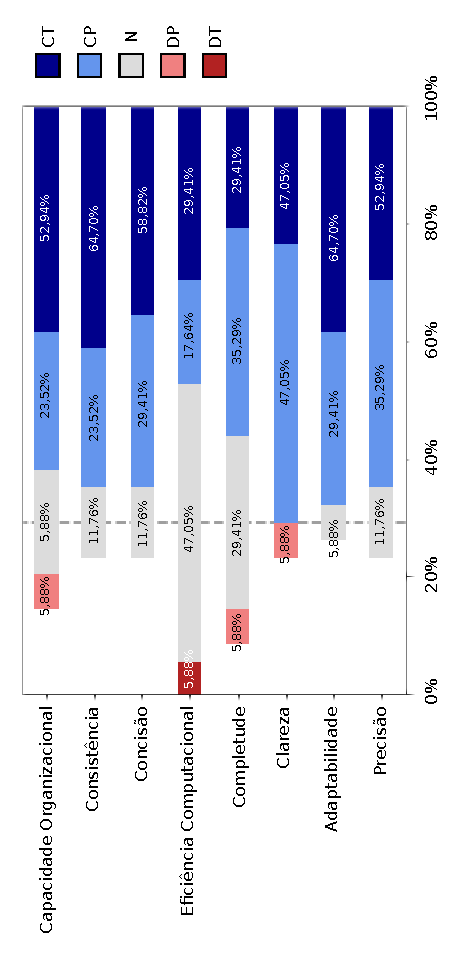
\includegraphics[angle=270,scale=1]{frequencia-likert-2.pdf}}
    \label{fig:frequencia-likert}
    \source{o Autor}
\end{figure}	


\subsection{Teste de Normalidade}
\label{sec:teste-normalidade}

Para descrever o teste de normalidade dos resultados foi aplicada uma abordagem estat�stica do m�todo aditivo com uma vari�vel dependente (VD) cont�nua. A VD � o resultado da somat�ria do valor dado a cada crit�rio por especialista. A \ref{tab:sum-especialistas} apresenta esses valores.

\begin{table}[]
    \centering
    \caption{Somat�rio das Resposta dos Especialistas}
    \label{tab:sum-especialistas}
    \begin{tabular}{@{}cc@{}}
    \toprule
    \textbf{Especialista (E)} & \textbf{Somat�rio dos Crit�rios} \\ \midrule
    E1 & 32 \\
    E2 & 37 \\
    E3 & 30 \\
    E4 & 32 \\
    E5 & 34 \\
    E6 & 40 \\
    E7 & 37 \\
    E8 & 37 \\
    E9 & 32 \\
    E10 & 31 \\
    E11 & 30 \\
    E12 & 25 \\
    E13 & 35 \\
    E14 & 34 \\
    E15 & 39 \\
    E16 & 37 \\
    E17 & 38 \\ \bottomrule
    \end{tabular}
    \source{o Autor}
\end{table}

Foram plotados esses valores no gr�fico de histograma apresentado na \ref{fig:histograma}. � necess�rio executar o teste de normalidade. Para isso foi usado o teste de Shapiro-Wilk \cite{shapiro1965analysis}. O teste Shapiro-Wilk testa a hip�tese nula de que os dados foram extra�dos de uma distribui��o normal, considerando que \textit{p-value} $>$ 0,05. 

\begin{figure}[H]
	\centering					
	\caption{Histograma da Somat�ria}
	{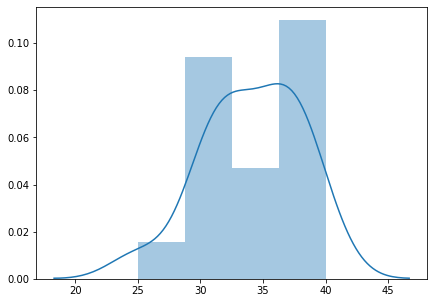
\includegraphics[scale=.8]{curva-normal.png}}
    \label{fig:histograma}
    \source{o Autor}
\end{figure}	


O resultado do teste estat�stico de Shapiro-Wilk foi 0,94 e o \textit{p-value} foi 0,44. Sendo assim, a distribui��o da VD � considerado \textbf{normal}.


\subsection{Teste de Hip�tese}
\label{sec:teste-hipotse}

Considerando que a amostra de VD segue uma distribui��o normal, pode-se aplicar o teste param�trico de Mann-Whitney \cite{mann1947test}. Para aplicar este teste foi preciso elaborar hip�teses para este question�rio. Considera-se que \textit{p-value:} $>$ 0,05 pode-se rejeitar H0 e quando p-value $<$ 0,05 n�o se rejeita H0.

O primeiro par de hip�tese � em rela��o a \textbf{N�vel de Forma��o} dos especialistas:

\begin{itemize}
    % \item \textbf{Hip�tese 1:} Existe diferen�a no resultado dado o N�vel de Forma��o?
    \item \textbf{Hip�tese Nula (H0):} n�o existe diferen�a na forma��o do especialista com rela��o a VD.
    \item \textbf{Hip�tese Alternativa:} existe diferen�a significativa na forma��o do especialista com rela��o a VD.
\end{itemize}

O resultado do teste de Mann-Whitney foi u = 0,000, p-value = 0,00000029 $<$ 0,05, logo � poss�vel rejeitar H0 e afirmar que, \textbf{existe diferen�as nos resultado dado o N�vel de Forma��o}.

O outro par de hip�tese � em rela��o a \textbf{Experi�ncia em LPS e/ou Ontologias (em anos)} dos especialista:

\begin{itemize}
    \item \textbf{Hip�tese Nula (H0):} n�o existe diferen�a na experi�ncia do especialista com rela��o a VD.
    \item \textbf{Hip�tese Alternativa:} existe diferen�a significativa na experi�ncia do especialista com rela��o a VD.
\end{itemize}

Para realiza��o deste teste foi necess�rio criar 3 grupos representativos dos anos de experi�ncia, os grupos s�o:

\begin{itemize}
    \item \textbf{1:} 0 � 5 anos de experi�ncias;
    \item \textbf{2:} 6 � 10 anos de experi�ncias; e
    \item \textbf{3:} 11 � 15 anos de experi�ncias.
\end{itemize}

O resultado do teste de Mann-Whitney foi u = 0,000, p-value = 0,00000027 $<$ 0,05, logo � poss�vel rejeitar H0 e afirmar que \textbf{existe sim diferen�as nos resultado dado o Experi�ncia em LPS e/ou Ontologias (em anos)}. 


\subsection{Correla��o dos Crit�rios}
\label{sec:correlacao-criterios}

Foi aplicado a t�cnica de correla��o de Pearson \cite{pearson}, pode-se realizar a seguinte interpreta��o:

\begin{itemize}
    \item \textbf{0.9} para mais ou para menos indica uma correla��o muito forte.
    \item \textbf{0.7 a 0.9} positivo ou negativo indica uma correla��o forte.
    \item \textbf{0.5 a 0.7} positivo ou negativo indica uma correla��o moderada.
    \item \textbf{0.3 a 0.5} positivo ou negativo indica uma correla��o fraca.
    \item \textbf{0 a 0.3} positivo ou negativo indica uma correla��o desprez�vel
\end{itemize}

A \ref{fig:correlacao} apresenta um mapa de calor indicando o grau de correla��o entre os crit�rios de qualidade. Foi poss�vel observar que os crit�rios com maior grau de correla��o foram \textbf{Completude} com \textbf{Precis�o} com o valor de correla��o forte \textbf{0,74}, \textbf{Capacidade Organizacional} com \textbf{Completude} com o segundo valor de correla��o forte \textbf{0,73} e \textbf{Consist�ncia} com \textbf{Concis�o} com o terceiro maior valor de correla��o moderada \textbf{0,70}.

\begin{figure}[H]
	\centering					
	\caption{Correla��o dos crit�rios de avalia��o.}
	{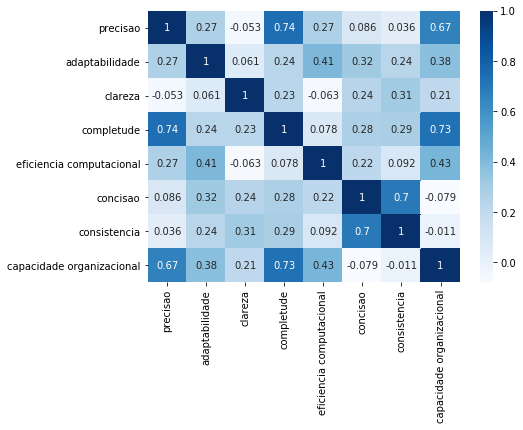
\includegraphics[scale=.8]{correlacao-criterios.png}}
    \label{fig:correlacao}
    \source{o Autor}
\end{figure}

\begin{table}[H]
    \centering
    \caption{\textit{Ranking} de correla��o dos crit�rios de avalia��o}
    \label{tab:correlacao-criterios}
    \begin{tabular}{@{}rllrc@{}}
    \toprule
    \multicolumn{1}{c}{\textbf{Posi��o}} & \textbf{Crit�rio Y} & \textbf{Crit�rio X} & \multicolumn{1}{c}{\textbf{Valor}} & \textbf{Interpreta��o} \\ \midrule
    1 & Completude & Precis�o & 0,74 & forte \\
    2 & \begin{tabular}[c]{@{}l@{}}Capacidade \\ Organizacional\end{tabular} & Completude & 0,73 & forte \\
    3 & Consist�ncia & Concis�o & 0,70 & forte \\
    4 & \begin{tabular}[c]{@{}l@{}}Capacidade \\ Computacional\end{tabular} & \begin{tabular}[c]{@{}l@{}}Efici�ncia \\ Computacional\end{tabular} & 0,43 & fraca \\
    5 & \begin{tabular}[c]{@{}l@{}}Efici�ncia \\ Computacional\end{tabular} & Adaptabilidade & 0,41 & fraca \\
    6 & \begin{tabular}[c]{@{}l@{}}Capacidade \\ Computacional\end{tabular} & Adaptabilidade & 0,38 & fraca \\
    7 & Concis�o & Adaptabilidade & 0,32 & fraca \\
    8 & Consist�ncia & Clareza & 0,31 & fraca \\
    9 & Consist�ncia & Completude & 0,29 & desprez�vel \\
    10 & Concis�o & Completude & 0,28 & desprez�vel \\
    11 & Adaptabilidade & Precis�o & 0,27 & desprez�vel \\
    12 & \begin{tabular}[c]{@{}l@{}}Efici�ncia \\ Computacional\end{tabular} & Precis�o & 0,27 & desprez�vel \\
    13 & Completude & Adaptabilidade & 0,24 & desprez�vel \\
    14 & Consist�ncia & Adaptabilidade & 0,24 & desprez�vel \\
    15 & Concis�o & Clareza & 0,24 & desprez�vel \\
    16 & Consist�ncia & Adaptabilidade & 0,24 & desprez�vel \\
    17 & Completude & Clareza & 0,23 & desprez�vel \\
    18 & Concis�o & \begin{tabular}[c]{@{}l@{}}Efici�ncia \\ Computacional\end{tabular} & 0,22 & desprez�vel \\
    19 & \begin{tabular}[c]{@{}l@{}}Capacidade \\ Computacional\end{tabular} & Clareza & 0,21 & desprez�vel \\
    20 & Consist�ncia & \begin{tabular}[c]{@{}l@{}}Efici�ncia \\ Computacional\end{tabular} & 0,092 & desprez�vel \\
    21 & Concis�o & Precis�o & 0,086 & desprez�vel \\
    22 & \begin{tabular}[c]{@{}l@{}}Efici�ncia \\ Computacional\end{tabular} & Completude & 0,078 & desprez�vel \\
    23 & Clareza & Adaptabilidade & 0,061 & desprez�vel \\
    24 & Consist�ncia & Precis�o & 0,036 & desprez�vel \\
    25 & \begin{tabular}[c]{@{}l@{}}Capacidade \\ Organizacional\end{tabular} & Consist�ncia & -0,011 & desprez�vel \\
    26 & Consist�ncia & Precis�o & -0,053 & desprez�vel \\
    27 & \begin{tabular}[c]{@{}l@{}}Efici�ncia \\ Computacional\end{tabular} & Clareza & -0,063 & desprez�vel \\
    28 & \begin{tabular}[c]{@{}l@{}}Capacidade \\ Organizacional\end{tabular} & Concis�o & -0,079 & desprez�vel \\ \bottomrule
    \end{tabular}
    \source{o Autor}
\end{table}

A \ref{tab:correlacao-criterios} apresenta o \textit{ranking} de correla��o dos crit�rios. Segundo a interpreta��o de \citet{pearson} s� ser�o consideradas as correla��es de 1 a 8 no \textit{ranking}. Dessa forma, pode-se afirmar que: 

\begin{itemize} 
    \item quanto melhor a \textbf{Completude} melhor a \textbf{Precis�o};
    \item quanto melhor a \textbf{Consist�ncia} melhor a \textbf{Concis�o};
    \item quanto melhor a \textbf{Capacidade Computacional} melhor a \textbf{Efici�ncia Computacional};
    \item quanto melhor a \textbf{Efici�ncia Computacional} melhor a \textbf{Adaptabilidade};
    \item quanto melhor a \textbf{Capacidade Computacional} melhor a \textbf{Adaptabilidade};
    \item quanto melhor a \textbf{Concis�o} melhor a \textbf{Adaptabilidade};
    \item quanto melhor a \textbf{Consist�ncia} melhor a \textbf{Clareza}; e
    \item quanto melhor a \textbf{Consist�ncia} melhor a \textbf{Completude}.
\end{itemize}

Os valores de correla��o negativa n�o foram o suficiente para serem considerados. Dessa forma, pode-se afirmar n�o existe  crit�rios com avalia��es inversas, como por exemplo, quanto melhor a \textbf{Efici�ncia Computacional} pior a \textbf{Concis�o}.


\section{Discuss�o dos Resultados}
\label{sec:discussao_dos_resultados}

Na Se��o \ref{sec:perfil-especialista} foi relatado o perfil dos especialista, pode-se notar que os especialistas possuem em m�dia 7,2 anos de experi�ncia em LPS e/ou Ontologias e que 70,61\% s�o doutores e P�s-doutores. Tal resultado corrobora para o alto grau de especialidades dos participantes.

Durante a Se��o \ref{sec:frequencia-likert} foi apresentado os resultados do estudo a an�lise dos demonstra que, segundo os especialistas, a onto possui um grau de qualidade relevante. Isso fica claro quando visualizamos que 70,15\% das respostas foram ``positivas'', ou seja, est�o entre CP e CT, o crit�rio \textbf{Adaptabilidade} se destacou nessa avalia��o. E apenas 2,95\% foram ``negativas'', ou seja, est�o entre DP e DT. Por�m o valor de 16,91\% no elemento N apresenta um ponto de aten��o, vimos que o crit�rio de qualidade que mais afetou este item foi a \textbf{Efici�ncia Computacional}. Estes valores est�o destacado na \ref{tab:total-respostas}

\begin{table}[htb]
    \centering
    \caption{Total de respostas positivas, neutras e negativas}
    \label{tab:total-respostas}
    \begin{tabular}{cccc}
    \hline
    \textbf{} & \textbf{Negativo (DT e DP)} & \textbf{Neutro (N)} & \textbf{Positivo (CP e CT)} \\ \hline
    Total de respostas & 4 & 23 & 109 \\
    \% & 2,95\% & 16,91\% & 70,15\% \\ \hline
    \end{tabular}
    \source{o Autor}
\end{table}

A Se��o \ref{sec:frequencia-likert} foi aplicado o m�todo aditivo para elaborar uma vari�vel dependente. Por meio do teste de Shapiro-Wilk pode-se identificar e a VD � uma distribui��o normal. Uma distribui��o normal apresenta que os dados est�o distribu�dos em 68,26\% por 1 desvio, um conjunto central, 95,44\% por 2 desvios e 99,73\% por 3 desvios. Sendo assim essa informa guia a proximos t�cnica de testes de hip�tese.

Logo, na Se��o \ref{sec:teste-hipotse} foram elaboradas duas hip�teses para averigua��o por meio de teste estat�stico de hip�tese. Primeira hip�tese \textbf{n�o existe diferen�a na forma��o do especialista com rela��o a VD} que por meio do teste de Mann-Whitney retornou \textit{p-value} $<$ 0,05, dessa forma rejeitando H0, tal resultado demonstra que a VD tem impacto sobre a forma��o do especialista. Segunda hip�tese: \textbf{n�o existe diferen�a na experi�ncia do especialista com rela��o a VD}, que por meio do teste de Mann-Whitney retornou o \textit{p-value} $<$ 0,05, da mesma forma que o anterior, rejeita H0, tal resultado demonstra que a VD tem impacto sobre a forma��o os anos de experi�ncia do especialista.

Por fim foi na Se��o \ref{sec:correlacao-criterios} apresenta o n�vel de correla��o entre os crit�rios, segundo as respostas dos especialistas. Foi poss�vel notar que das 28 possibilidades s� foram encontradas correla��es relevantes em oito delas. Foi elaborado um \textit{ranking} das correla��es, por meio dele foi poss�vel identificar quais crit�rios atacar em conjunto para potencializar a uma melhoria na ontologia.

Feito essa an�lise � poss�vel afirmar que a OntoExper-SPL � altamente adapt�vel a novas extens�es, tornando ela coesa e de f�cil extens�o a novos axiomas. Por�m constata-se que h� uma falha com rela��o a efici�ncia computacional, ou seja, ela n�o possui um bom desempenho em sua execu��o (execu��o de infer�ncias).


\section{Amea�as � Validade}
\label{sec:ameca_a_validade}

Esta se��o discute a validade identificadas durante o estudo. Para apresentar as amea�as � validade, foram categoriza-los
em interna, externa, de constructo e de conclus�o, de acordo com \citet{wohlin2012}.

\subsection{Amea�as � Validade Interna}

A seguir est�o listadas as amea�as a validade interna:

\begin{itemize}
    \item \textbf{Diferen�as entre os especialistas:} devido do tamanho da amostra, as varia��es entre as habilidades dos especialistas foram poucas, assim, os especialistas n�o foram divididos em grupos. Dessa forma, as tarefas designadas foram id�nticas;
    
    \item \textbf{Acur�cia das respostas dos participantes:} uma vez que as informa��es referentes da OntoExper-SPL  s�o apresentadas juntamente com seus metadados e considerando que os participantes s�o especialistas em ES, LPS e Ontologia, considera-se que as respostas fornecidas s�o v�lidas;
    
    \item \textbf{Efeito de Fadiga:} os arquivos da OntoExper-SPL (modelagem e povoados com indiv�duos) s�o de dif�cil leitura pelos seres humanos, logo se faz necess�ria a utiliza��o de ferramentas para exibi��o da OntoExper-SPL, bem como os textos auxiliares, para uma maior compreens�o dos crit�rios de avalia��o, e das imagens anexadas ao question�rio. Os efeitos de fadiga s�o uma das principais amea�as, por isso, para tentar minimizar esse problema, a documenta��o foi enviada aos especialistas por e-mail com um prazo de 40 dias para enviarem as respostas, assim, eles poderiam responder conforme a sua disponibilidade;
    
    \item \textbf{Influ�ncia de outros especialistas na avalia��o:} a influ�ncia entre os especialistas foi mitigada, pois eles n�o sabiam quem foram convidados para tal estudo; e
    
    \item \textbf{An�lise dos dados:} em rela��o ao crit�rio de avalia��o \textbf{Efici�ncia Computacional} existe uma amea�a pois os participantes relataram que n�o foi poss�vel executar a tarefa, para tentar minimizar esse problema, a escala Likert atribui o valor N, considerando com baixa signific�ncia no resultado. A an�lise dos dados dos especialistas foi realizada somente pelo autor desta disserta��o, sem a realiza��o de uma revis�o. Dessa forma, tal an�lise deve ser revisada em trabalhos futuros.
\end{itemize}


\subsection{Amea�as � Validade Externa}

A obten��o de especialistas qualificados nas �rea de ES, LPS e Ontologia foi uma das dificuldades encontradas neste estudo e muitos especialistas convidados n�o puderem participar do estudo por conta dos seus compromissos. Apesar de poucos especialistas participarem do estudo, a qualidade do perfil deles � a vari�vel mais importante nessa avalia��o.

\subsection{Amea�as � Validade de \textit{Constructo}}

A instrumenta��o foi avaliada e adequada, conforme projeto piloto realizado. Quanto ao n�vel de conhecimento dos especialistas em ES, LPS e Ontologia demonstraram satisfat�rios para avaliarem as diretrizes propostas. Os especialistas que n�o tinha familiaridade com Ontologia, pode encontrar no material de apoio um respaldo para execu��o das tarefas.

\subsection{Amea�as � Validade de Conclus�o}

A principal amea�a para este estudo est� relacionada ao n�mero de especialistas (17). Este n�mero � pequeno, mas o conhecimento dos especialistas que colaboraram com este estudo foi significativo. Al�m disso, pela caracter�stica pr�pria do estudo por prezar a qualidade dos especialistas, muitas vezes o n�mero baixo de especialistas pode ser considerado. Assim, n�o � poss�vel generalizar as conclus�es.


% TODO
\section{Empacotamento e Compartilhamento}
\label{sec:empacotamento_e_compartihamento}

Os documentos disponibilizados aos participantes e resultados deste estudo est�o dispon�veis em: https://doi.org/..., visando dissemina��o dos dados.


\section{Propostas de Melhorias com Base na Discuss�o dos Resultados}
\label{sec:propostas_de_melhorias}

Esta Se��o discute as melhorias apresentada pelos especialistas que participaram do estudo emp�rico, bem como armadilhas que a ferramenta OOPS!.

\subsection{Melhorias Apontada pelos Especialistas}

Durante a execu��o do estudo os especialistas puderam contribuir com um campo aberto a coment�rios gerais, neste campos eles comentaram os pontos positivos e negativos encontrado durante avalia��o dos crit�rios de qualidade:

\begin{itemize}
    \item Coment�rio do E4: 
    \begin{quotation}
        Acredito que a Ontologia esteja bastante gen�rica e adequada para o contexto da Engenharia de Software. Consegui navegar e me entender melhor os axiomas usando as ferramentas propostas (Prot�g� e WebVOWL), mas tive problemas ao tentar executar as queries SPARQL online (usando o http://atted.jp/sparql por exemplo).
    \end{quotation}
    
    \item Coment�rio do E5:
    \begin{quotation}
        As estruturas e rela��es foram bem estruturadas na ontologia. Os t�picos b�sicos de experimenta��o em engenharia de software est�o bem representados e associados a literatura b�sica de experimenta��o quantitativa.

        % O primeiro coment�rio, seria a altera��o de "OntoExper-SPL" para "SmartyOntology". � uma contribui��o para a abordagem Smarty certo?

        % A instrumenta��o dessa avalia��o foi validada em um estudo piloto? Acredito que a Ontologia poderia conter um t�pico chamado "Grupo de Controle" para avaliar a qualidade do experimento em LPS. Na maioria das vezes � dif�cil entender quais aspectos de determinadas tecnologias podem ser avaliadas em conjunto com LPS. Talvez criar Grupos de Controle como Academia ou Ind�stria e incluir os participantes em um estudo piloto. Tal grupo de controle pode estar associado a "Pilot Project" j� representado na ontologia. 

        Quanto aos termos, � necess�ria uma revis�o dos termos utilizados na Ontologia, por exemplo, "Keyworld" para "Keywords". 

        Na modelagem, a "SPL artifacts" est� sozinha, por que? Ser� que poderia estar associada ao "SPL domain"? 

        Senti falta de "Results" que poderia estar associada de algum modelo com "Discussion". Acredito que isso poderia ser uma recomenda��o de melhoria para a ontologia.

        Pensando an�lise qualitativa dos dados, acho que nenhuma modelagem ou representa��o foi criada em "Analyze" na Ontologia? 

        Hoje existe um grande interesse na comunidade cient�fica em an�lises qualitativas, uma sugest�o seria estender a OntoExper-SPL para tal contexto de an�lise. Entretanto, eu entendo que a ontologia foi proposta para experimentos quantitativos, mas isso poderia ser uma extens�o ou trabalho futuro bem interessante para a comunidade cient�fica de LPS ou at� mesmo para a �rea de Ontologia em geral.
    \end{quotation}

    \item Coment�rio do E8:
    \begin{quotation}
        O entendimento da ontologia � f�cil para aqueles que conhecem o dom�nio de experimenta��o em engenharia de software e a sub�rea de linha de produto de software.
    \end{quotation}

    \item Coment�rio do E10:
    \begin{quotation}
        Gostaria apenas de comentar um detalhe. O id da ontologia tem um typo: "experiemnt". 
    \end{quotation}

    \item Coment�rio do E11:
    \begin{quotation}
        Achei confusa a nota��o para expans�o da documenta��o.
        Senti falta de cobrir os tipos de estudo (prim�rios, secund�rios e terci�rios)
        Assim como, notei a aus�ncia de "Amea�as a Validade".
        Os pesquisadores se baseiam somente no Wohlin, sugiro que olhem outras propostas e refer�ncias para complementar os dom�nios e aplica��es.
    \end{quotation}
    
    \item Coment�rio do E13:
    \begin{quotation}
        O question�rio est� muito denso, e parece ser necess�rio ter usado a ontologia para responder de uma maneira apropriada. Ficou muito pesado.
    \end{quotation}
    
    \item Coment�rio do E15:
    \begin{quotation}
        Do meu conhecimento em experimenta��o e em LPS eu considero que a ontologia proposta est� coerente e satisfatoriamente modelada. Senti falta da modelagem dos "subjects" envolvidos no experimento. N�o sei esse conceito foi modelado com outro nome e eu n�o identifiquei, se n�o foi inclu�do intencionalmente ou se foi esquecido. 
    \end{quotation}

    \item Coment�rio do E16:
    \begin{quotation}
        Talvez seja interessante modificar a classe Package para ReplicationPackage ou algum termo relacionado com Open Science.
    \end{quotation}

    \item Coment�rio do E17:
    \begin{quotation}
        Me deparei com o problema da defini��o do Reasoner para executar a query. Se executado no arquivo que n�o est� populado, o resultado da query atende aos 2s esperados, contudo, ao meu ver uma query que limita-se em retornar apenas o nome das classes relacionadas n�o � v�lida para  a utiliza��o da ontologia definida. Como tal problema pode ser resultado de algo espec�fico na configura��o do ambiente de execu��o (o qu� acredito que n�o seja o caso), assinalei a op��o 3.

        Executando a query: Experiment and ExperimentSPL and pagesNumber value 8 n�o obtive resultado, mesmo tendo navegado e visualizado que h� respostas que satisfa�am tal pesquisa. Adicionalmente, depois de selecionar para inicializar o reasoner e, ap�s alguns minutos ser apresentada uma lista de inconsist�ncias (para o arquivo \\smart-ontology-populate-validated.owl), o Protege para de responder.

        Tentei executar ainda a query presente no artigo da ontologia, tamb�m sem sucesso. 

        % Inconsist�ncia no pacote enviado: O arquivo enviado por e-mail n�o � o mesmo do dispon�vel no drive (link na primeira p�gina do formul�rio), visto que a planilha de dados n�o se encontra no mesmo.

        Ainda sobre o processo de avalia��o, a defini��o de queries para serem executadas deveriam estar mais expl�citas.         
    \end{quotation}
    
\end{itemize}

No geral foi poss�vel notar que a OntoExper-SPL precisa ser melhorada quanto a sua efici�ncia computacional. Os pontos de melhoria s�o, corrigir os termos \textit{Keyworld} para \textit{Keywords}, associar \textit{SPL  artifacts} a \textit{SPL domain}, incluir os axiomas \textit{Results}, \textit{Analyze}, ``Amea�as a Validade'', \textit{Subjects}e modificar o axioma \textit{Package} para \textit{Replication-Package}.

\subsection{Melhorias com Base em Armadilhas Identificadas na Ferramenta do OOPS!}

Na \ref{tab:result_of_evaluation} foi relatado as armadilhas que a ferramenta encontrou na OntoExper-SPL, a seguir est�o descritos as melhorias que devem ser realizada na ontologia para melhorar estes pontos:

\begin{itemize}
    \item No caso \textbf{P08:} deve-se criar anota��es para os axiomas;
    \item No caso \textbf{P10:} deve-se criar as disjun��es dos axiomas;
    \item No caso \textbf{P13:} deve-se criar relacionamentos inverso para os axiomas: \textit{typeSelectionOfParticipants, typeExperimentSPL, typeExperiment, typeDesignExperiment, typeContextSelection, typeContextExperiment, experiment, documentation};
    \item No caso \textbf{P19:} deve-se remover os dom�nios e alcances desnecess�rios para os axiomas: \textit{documentation, experiment, typeContextExperiment, typeDesignExperiment, typeExperiment, typeSelectionOfParticipants}; 
    \item No caso \textbf{P41:} deve-se atribuir uma licen�a a OntoExper-SPL.
\end{itemize}    

\section{Considera��es Finais}
\label{sec:concidaracoes_finais}

Este cap�tulo apresentou a avalia��o quantitativa sobre oito crit�rios de qualidade aplicados a OntoExper-SPL com especialistas em ES, LPS e Ontologia. Os resultados obtidos permitiram identificar a qualidade da OntoExper-SPL. Assim, os resultados dos dados analisados forneceu evid�ncias que as OntoExper-SPL possui um grau de qualidade relevante. Permitindo assim a evolu��o de novos estudos sobre a OntoExper-SPL, expandindo-a e melhorando seus pontos de baixa qualidade.

Foram sugeridas melhorias � OntoExper-SPL, tanto pelos especialistas como pela ferramenta OOPS!, que devem ser aplicadas em trabalhos futuros. Por fim, compreende-se que novos estudos devem ser realizados com outros especialistas para expandir o corpo de conhecimento.
\chapter{Prot�tipo de um Sistema de Recomenda��o para OntoExer-SPL}
\pagestyle{plain}
\label{sec:recsys}


\section{Considera��es Iniciais}
\label{sec:concideracoes_iniciais}

Este cap�tulo apresenta um prot�tipo de Sistema de Recomenda��o (SR) para a realiza��o de infer�ncias no modelo de ontologia proposto neste trabalho de mestrado, a OntoExper-SPL. O prot�tipo serve como uma forma de demonstrar a import�ncia do modelo ontol�gico e tamb�m como uma forma de avalia a viabilidade de SR para experimento de LPS.

% , por meio de uma implementa��o de um sistema de recomenda��o (SR). Dessa forma a estrutura deste cap�tulo fica, na Se��o \ref{sec:sistema_de_recmendacao} apresenta um breve contexto sobre SR e sua origem, seus principais modelos de implementa��o e como os SR s�o visto pela ES; na Se��o \ref{sec:concepcao_recsys}apresenta como as consultas iniciais na OntoExper-SPL levou a implementa��o do SR e como ele encaixa como motor de infer�ncia na OntoExper-SPL, bem como sua intera��o com o usu�rios; na Se��o \ref{sec:projeto_recsys} apresenta as quatro fase de constru��o SR, (i) a \textbf{Fase 1} apresenta a cria��o do projeto de sistema web usando Django Framework e a implementa��o de um prototipa��o da tela de itera��o do usu�rio com SR, (ii) a \textbf{Fase 2} apresenta como a OntoExper-SPL � carregada no SR e como foi implementado os mecanismos de consultas na OntoExper-SPL, a \textbf{Fase 3} apresenta implementa��o da avalia��o dos usu�rios no SR e como esta � armazenado no SR, esta avalia��o � denominada \textit{Ratings}, por fim a \textbf{Fase 4} apresenta com foi implementado do modelo de recomenda��o, na qual, foi usado  o conceito de filtragem colaborativa aplicando c�lculo da dist�ncia Euclidiana, bem como tamb�m apresenta como foi implementa��o a quest�o da da partida fria do modelo de recomenda��o para novos usu�rios; na Se��o \ref{sec:ambiente_de_desenvolvimento} apresenta quais foram as tecnologias e ferramentas usadas para o desenvolvimento do SR;


\section{Sistema de Recomenda��o}
\label{sec:sistema_de_recmendacao}

Os sistemas de recomenda��o s�o aplicativos de software que visam dar suporte para o usu�rio na tomada de decis�es ao interagir com grandes espa�os de informa��o. Esses softwares recomendam itens de interesse para os usu�rios com base em prefer�ncias que tenham sido expressas explicita ou implicitamente \cite{ricci2011introduction}. Segundo \citet{mahmood2009improving} os sistemas de recomenda��o s�o t�cnicas ou ferramentas de software, que podem reduzir a sobrecarga de informa��es para os usu�rios, sugerindo itens, conte�dos ou servi�os, entre outros.

Os sistemas de recomenda��o surgiram nos trabalhos extensivos das ci�ncias cognitivas, teoria de aproxima��o, recupera��o da informa��o e teoria de previs�es e tamb�m possuem influ�ncias das ci�ncias de administra��o e marketing \cite{allen2001econometric, murthi2003role}. O primeiro sistema de recomenda��o proposto que se tem conhecimento, foi o \textit{Tapestry}. Nesse sistema criou-se o modelo mais usado em sistemas de recomenda��o, em que  a recomenda��o de conte�do � auxiliada pela colabora��o de um grupo de pessoas, batizado como ``filtragem  colaborativa''. Neste trabalho, iniciou-se o desafio de congregar corretamente os dados recomendados com os usu�rios que o recebem, analisando o real relacionamento de interesse \cite{kwong1992dynamic, resnick1997recommender}.

Uma defini��o formal para sistema de recomenda��o �: 

\newtheorem{mydef}{Defini��o}
\begin{mydef}
	Seja $C$ o conjunto de todos os usu�rios de um determinado sistema, e seja $S'$ o conjunto de todos os poss�veis itens que podem ser recomendados como livros, filmes, restaurantes etc. Seja $u$ a fun��o utilidade que mede o qu�o �til � um determinado item s para um determinado usu�rio $c$, \textbf{\textit{u}:C x S $\rightarrow$ R}, onde $R$ � um conjunto totalmente ordenado segundo a fun��o utilidade. Ent�o, para cada usu�rio \textbf{\textit{c} $\in$ C}, procura-se um item \textbf{\textit{s'} $\in$ S} que maximiza a utilidade do usu�rio. Isto pode ser expressado pela equa��o \ref{eq:form_sis_rec}:
	
	\begin{equation}
	\label{eq:form_sis_rec}
	\forall c \in C, s'_{c} = argmax_{s \in S u(c, s)}
	\end{equation}
	
\end{mydef}

Em um sistema de recomenda��o a utilidade de um item � geralmente representada por uma avalia��o que indica o quanto um determinado usu�rio gosta de um item. No entanto, conforme descrito na defini��o acima, a fun��o de utilidade pode ser uma fun��o arbitr�ria.

Cada elemento dos usu�rios $C$ pode ser definido por um perfil que inclui as caracter�sticas do usu�rio, por exemplo, a sua idade, sexo, etc. No caso mais simples, o perfil pode conter um �nico elemento como um identificador �nico (ID). Da mesma forma, cada item de $S$ pode ser definido por um conjunto de caracter�sticas. Por exemplo, na recomenda��o de filmes, na qual $S$ � a cole��o de filmes, cada filme pode ser representado n�o apenas pelo seu ID, mas tamb�m pelo seu t�tulo, g�nero, diretor, ano de lan�amento, etc.

Existem cinco abordagens mais usadas em sistemas de recomenda��o, Tr�s consideradas como tradicionais: Filtragem Colaborativa (\textit{Collaborative Filtering}), Filtragem Baseada em Conte�do (\textit{Content-based Filtering}) e Recomenda��o Baseada no Conhecimento (\textit{Knowledge-Based Recommendation}). Duas consideradas mais atuais: Sistemas de Recomenda��o H�bridos \textit{(Hybrid Recommender Systems}) e Sistemas de Recomenda��o usando Informa��es de Contexto (\textit{Context-aware Recommender Systems}). 


\subsection{\textit{Collaborative Filtering}}
\label{sec:collaborative_filtering}

A Filtragem Colaborativa baseia-se na id�ia de ``boca-a-boca'' em que a informa��o passada de pessoa a pessoa desempenha um papel importante ao tomar uma decis�o. Abstraindo, as pessoas s�o substitu�das pelos, chamados, vizinhos mais pr�ximos (NN) que s�o usu�rios com um padr�o de prefer�ncia ou comportamento semelhante ao usu�rio atual \cite{robillard2010recommendation}. A filtragem Colaborativa depende de dois tipos diferentes de dados: (1) um conjunto de usu�rios e (2) um conjunto de itens. A rela��o entre usu�rios e itens � expressada principalmente em termos de \textit{ratings} fornecidos pelos usu�rios e explorados em futuras sess�es de recomenda��o para prever a classifica��o de um usu�rio \cite{robillard2010recommendation}. A \ref{fig:filtragem-colaborativa} apresenta o comportamento desse modelo.

\begin{figure}[htb]
	\centering 
	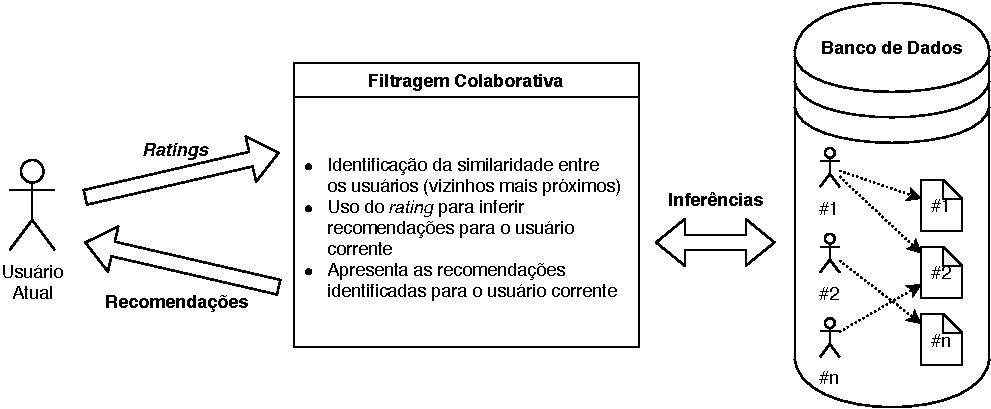
\includegraphics[scale=.9]{filtragem-colaborativa.pdf}
	\caption{Filtragem Colaborativa. Traduzido e Adaptado de \citet{robillard2010recommendation}}
	\label{fig:filtragem-colaborativa}
\end{figure}

Dado que este trabalho trata o sistema de recomenda��o como uma forma de realiza��o de infer�ncia sobre a OntoExper-SPL, utilizou-se a abordagem Filtragem Colaborativa.


\subsection{Sistemas de Recomenda��o em Engenharia de Software}

Em Engenharia de Software (\textit{Recommendation System in Software Engineering} - RSSEs), sistemas de recomenda��o desempenham importantes fun��es a fim de ajudar a equipe de software a lidar com sobrecarga de informa��es, filtrando e fornecendo informa��es �teis. S�o ferramentas de software introduzidas especificamente para ajudar equipes de desenvolvimento de software e partes interessadas a lidar com a busca de informa��es em um determinado contexto em ES \cite{robillard2010recommendation}.

\citet{robillard2010recommendation} comentam que, em um ambiente de desenvolvimento de software aplicando ES existe um ampla gama de informa��es sobre o projeto em desenvolvimento, e este espa�o de informa��es pode ser categorizados por:

\begin{itemize}
	\item C�digo fonte do projeto;
	\item Hist�ria do projeto;
	\item Arquivos de comunica��o;
	\item Depend�ncias de API em outras fontes;
	\item Ambiente de desenvolvimento;
	\item Logs de intera��o entre os usu�rios;
	\item Logs de execu��o e;
	\item A web.
\end{itemize}

Um RSSE pode trazer simultaneamente dois aspectos distintos: (i) novidade e surpresa, porque os RSSEs ajudam a descobrir novas informa��es e (ii) familiaridade e refor�o, pois as RSSEs suportam a confirma��o do conhecimento existente. Referenciar uma tarefa e um contexto espec�fico distingue RSSEs de ferramentas de pesquisa gen�ricas, por exemplo, uma ferramentas de RSSR para ajudar os desenvolvedores a encontrar exemplos de c�digo fonte \cite{robillard2010recommendation}.

Um RSSE compreende tr�s componentes principais, (i) um mecanismo para coletar dados, (ii) um mecanismo de recomenda��o para analisar dados e gerar recomenda��es e (iii) uma interface de usu�rio para fornecer recomenda��es \cite{rahman2014towards}.

\begin{figure}[htb]
	\centering					
	{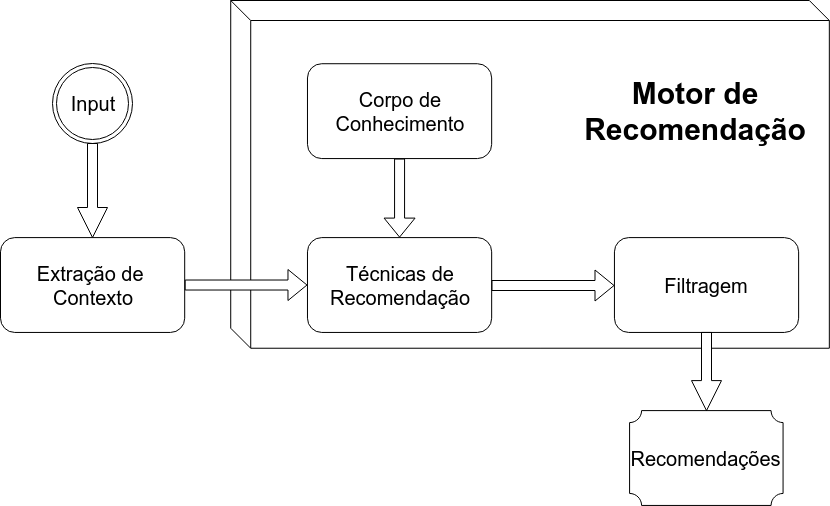
\includegraphics[scale=.5]{rsse.png}}
	\caption{Passos de Constru��o para um RSSE. Traduzido e Adaptado de \citet{maki2016systematic}}
	\label{fig:rsse}
\end{figure}

A \ref{fig:rsse} apresenta de forma geral como � constru�do um RSSE, partindo da entradas dos dados pelo \textit{input}, passando pela extra��o de contexto, seguindo para aplica��o de alguma t�cnica de recomenda��o, na qual sofre um infer�ncia do corpo de conhecimento (normalmente espec�fico para cada �rea de ES), depois segue para um processo de filtragem dos resultados, e como sa�da a recomenda��o em si.

Foi encontrada uma revis�o sistem�tica \cite{maki2016systematic}, que aborda m�todos e modelos de implementa��o de um RSSE apresentando v�rios aspectos de SR em ES, principalmente no tipo de corpo de conhecimento aplicado a RSSE. Nessa revis�o foi poss�vel identificar algumas �reas da ES que utilizam SR:

\begin{itemize}
	\item para explora��o c�digo fonte;
	\item para reuso de software;
	\item para refatora��o de c�digo fonte (por exemplo, \textit{class} em POO);
	\item para reuso de componentes de software;
	\item para explora��o de APIs;
	\item para depura��o de c�digo (\textit{debugging})
	\item para recomenda��o de agentes \textit{Agile}
	\item para descoberta de requisitos;
	\item para mudan�a do ciclo de vida;
	\item para evolu��o do ciclo de vida e;
	\item para busca de \textit{bugs}.
\end{itemize}

Por meio deste estudo, foi poss�vel identificar qual t�cnica de SR para qual dominio de aplica��o na industria.

\begin{landscape}
	\topskip0pt
    \vspace*{\fill}
	\begin{table}[]
		\centering
		\caption{Sum�rio de t�cnicas de recomenda��o em cada dom�nio, Traduzido e Adaptado de \citet{maki2016systematic} }
		\label{tab:tec_x_doman}
		\begin{tabular}{@{}llllllllll@{}}
			\toprule
			\multicolumn{1}{c}{\textbf{Dom�nios}} & \multicolumn{8}{c}{\textbf{T�cnicas}} & \multicolumn{1}{c}{\textbf{\begin{tabular}[c]{@{}c@{}}N�mero de \\ Refer�ncias\end{tabular}}} \\ \midrule
			& CBF & CF & KBF & Hibrido & IA & \begin{tabular}[c]{@{}l@{}}Redes \\ Sociais\end{tabular} & \begin{tabular}[c]{@{}l@{}}Info. de\\ Contexto\end{tabular} & \begin{tabular}[c]{@{}l@{}}Grupo de \\ agrega��o\end{tabular} &  \\ \midrule
			Governo & 1 & 5 & 1 & 5 & 4 &  &  &  & 9 \\
			Neg�cios &  & 1 & 3 & 3 & 4 &  &  &  & 5 \\
			Comercio & 3 & 1 & 4 & 1 & 4 & 2 &  &  & 8 \\
			Livraria & 2 & 2 &  & 3 & 1 &  &  &  & 6 \\
			Escolas & 2 &  & 11 &  & 1 &  &  &  & 10 \\
			Turismo & 5 & 9 & 9 & 9 & 2 & 2 & 11 &  & 18 \\
			Pesquisa & 9 & 16 & 6 & 15 & 3 & 1 & 1 &  & 27 \\
			\begin{tabular}[c]{@{}l@{}}Grupo de \\ Atividade\end{tabular} & 9 & 5 & 2 & 5 & 8 &  &  & 2 & 21 \\
			\textbf{Total} & \textbf{31} & \textbf{39} & \textbf{36} & \textbf{41} & \textbf{27} & \textbf{5} & \textbf{12} & \textbf{2} & \textbf{104} \\ \bottomrule
		\end{tabular}
	\end{table}
	\vspace*{\fill}
\end{landscape}


\section{Concep��o}
\label{sec:concepcao_recsys}

Ap�s o desenvolvimento da ontologia e seu povoamento, iniciou-se um processo emp�rico de valida��o dos dados inseridos, realizando infer�ncias a OntoExper-SPL por meio de consultas, como apresentado na Se��o \ref{sec:exemplo}. No decorrer deste estudo foi utilizada a biblioteca OWLReady2 para cria��o das consultas mais elaboradas, algumas destas serviram de bases para implementar o SR.

dadas essas considera��es iniciais sobre consultas preliminares na ontologia proposta, foi poss�vel esbo�ar um SR para realizar, como prova de conceito, infer�ncia na OntoExper-\\SPL. Dessa forma foi elaborado um projeto de SR que possa conectar os usu�rios aos itens (experimentos de LPS).

A \ref{fig:RSSE-overview} apresenta o conceito geral da metodologia deste projeto. Iniciando pela entrada dos usu�rios, depois extraem-se as prefer�ncias dele (por meio de ratings), e em seguida � realizada a extra��o de informa��es de contexto utilizando a base de metadados em LPS (OntoExper-SPL), para ent�o fazer infer�ncia nos itens. Por meio dessa infer�ncia � poss�vel obter as recomenda��es (itens ranqueadas para cada usu�rio).

\begin{figure}[htb]
	\centering					
	{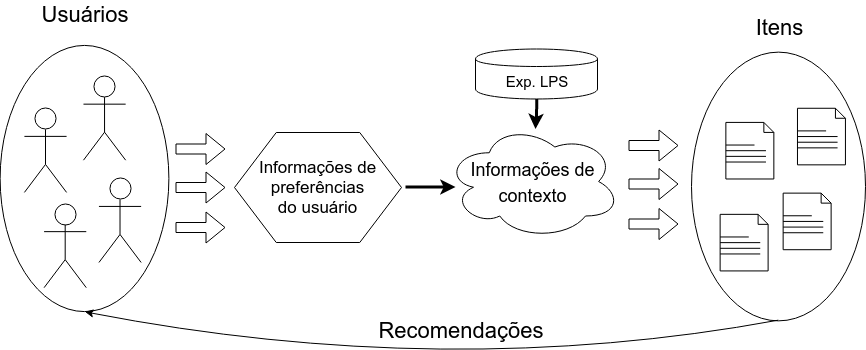
\includegraphics[scale=.5]{RSSE-overview.png}}
	\caption{Modelagem geral do SR como prova de conceito para OntoExer-LPS}
	\label{fig:RSSE-overview}
\end{figure}


Inicialmente, a entrada de dados dos usu�rios est� definida da seguinte forma:

\begin{itemize}
	\item Artefatos de LPS:
	\item Tipo do experimento LPS
\end{itemize}

Posteriormente, definiu-se algumas tecnologias para o desenvolvimento do SR, seguindo as boa pr�ticas de desenvolvimento de sistemas. Por meio dessas tecnologias foi poss�vel construir o SR descrito na pr�xima se��o.

\section{Projeto}
\label{sec:projeto_recsys}

Para o desenvolvimento do SR foi necess�rio encontrar tecnologias que atendessem os requisitos, tanto de SR como de ontologias. A linguagem de programa��o Python foi escolhida novamente por atender estes dois requisitos. Quanto a ontologia, Python j� foi utilizada para manipula��o da ontologia por meio da biblioteca OWLReady2. Quanto ao SR por possuir facilidade de implementa��o de algoritmos complexos e manipula��o de dados com Pandas. Um vi�s para esta implementa��o foi o conhecimento do pesquisador em desenvolvimento web, isso motivou o uso do Django Framework \footnote{https://djangoproject.com} para desenvolvimento web com Python. Dessa forma, toda \textit{stack} de desenvolvimento do SR foi baseada na linguagem Python.

O desenvolvimento deste projeto foi dividido em quatro fases:

\begin{itemize}
	\item \textbf{Fase 1:} cria��o do projeto de aplica��o web usando Django Framework e implementa��o de um prototipa��o da tela de intera��o com usu�rio;
	\item \textbf{Fase 2:} carregamento da OntoExper-SPL e implementa��o dos mecanismos de consultas;
	\item \textbf{Fase 3:} \textit{ratings} dos usu�rios e armazenamento da avalia��o no SR; e
	\item \textbf{Fase 4:} implementa��o do modelo de recomenda��o e implementa��o do conceito de filtragem colaborativa.
\end{itemize}

\subsection{Fase 1: O Projeto de SR Usando Django Framework}

Django Framework � um framework \textit{open source} para desenvolvimento de aplica��es web para linguagem Python. Ele  implementa o modelo para desenvolvimento em camadas chamado MTV \textit{(Model, Template, View)}. Este conceito � semelhante a arquitetura MVC \textit{(Model, View, Controller)} \cite{krasner1988description}, por�m com outra nomenclatura. A seguir � descrita qual a responsabilidade de cada camada no Django:

\begin{itemize}
	\item \textbf{A camada do modelo:} fornece uma camada de abstra��o para estruturar e manipular os dados da aplica��o da web;
	\item \textbf{A camada de visualiza��o:} tem o conceito de "visualiza��es" para encapsular a l�gica respons�vel pelo processamento da solicita��o de um usu�rio e pelo retorno da resposta; e
	\item \textbf{A camada de template:} fornece uma sintaxe amig�vel para o desenvolvedor renderizar as informa��es a serem apresentadas ao usu�rio.
\end{itemize}

Al�m de implementar este padr�o de modelo de desenvolvimento, o Django oferece outras caracter�sticas, como um processo intuitivo e claro de configura��o por meio de um arquivo \textit{settings.py}, a possibilidade de encapsulamento de processos com cria��o de pequenas aplica��es dentro do projeto, possibilidade de internacionaliza��o, implementa��o de autentica��o e seguran�a, configura��o de \textit{timezone}, al�m de uma implementa��o pronta para administra��o da aplica��o, chamado Django Admin. 

Uma das parte do Django admin � o site, ela oferece a gera��o de p�ginas autom�ticas com base nos metadados dos modelos de neg�cio criado pelo desenvolvedor.

Outro recurso que o Django tr�s � parte de autentica��o de seguran�a, por meio deste recurso � poss�vel criar e gerenciar contas de usu�rios, grupo de usu�rios, permiss�es de acesso e os \textit{cookies} de sess�o do usu�rio.

Dessa forma, com o Django Framework, foi poss�vel implementar um SR robusto, garantindo as principais funcionalidades de uma aplica��o web. 

A aplica��o constru�da conta com a seguinte �rvore de diret�rios apresentada na \ref{figure:dir-recsys-onto}

\begin{figure}[htb]
	\centering 
	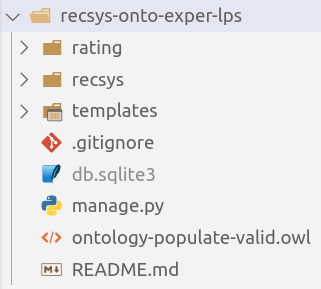
\includegraphics[scale=1]{dir-recsys-onto.png}
	\caption{�rvore de diret�rios da aplica��o SR com Django Framework.}
	\label{figure:dir-recsys-onto}
\end{figure}

O diret�rio \lstinline{recsys-onto-exper-lps} � o diret�rio raiz do projeto, todo c�digo fonte da aplica��o se encontra nele.

O diret�rio \lstinline{ratings} � uma aplica��o dentro do projeto, nela cont�m a modelagem de dados para o armazenamento das avalia��es dos usu�rios

O diret�rio \lstinline{recsys} � o diret�rio de configura��o principal do projeto, nela cont�m o arquivo \textit{settings.py} (confiugura��o global do projeto) e \textit{views.py} que � o principal aquivo deste projeto. Nele cont�m toda regra e controle das funcionalidades implementada neste projeto - nas pr�ximas subse��es ser� detalhada estas funcionalidades. Neste diret�rio tbm cont�m o arquivo \textit{collaborativeFilter.py} que implementa o modelo de recomenda��o.

O diret�rio \lstinline{templates} � o diret�rio respons�vel por encapsular todas as partes da �nica tela que o projeto implementa. S�o cinco arquivos HTML que s�o apresentados em uma �nica tela para o usu�rio no navegador.

O arquivo \textit{.gitignore} � respons�vel por configurar quais arquivos e diret�rios n�o ser�o versionados pelo sistema de controle de versionamento (Git).

O arquivo \textit{db.sqlite3} � pr�prio banco de dados. O banco de dados do projeto ser� detalhado na Se��o \ref{sec:banco_dados}.

O arquivo \textit{manage.py} � respons�vel por prover a execu��o da aplica��o Django Framework.

O arquivo \textit{ontology-populate-valid.owl} � a pr�pria OntoExper-SPL povoada com seus indiv�duos, na qual o projeto realiza infer�ncias.

O arquivo \textit{README.md} � um arquivo de marca��o que descreve o projeto.


\subsection{Fase 2: Carregamento da OntoExper-SPL no SR}

Como foi apresentado na se��o anterior, o arquivo \lstinline{ontology-populate-valid.owl} est� localizado na raiz do projeto, para o SR manusear este arquivo, foi preciso criar uma configura��o no arquivo \textit{settings.py} apresentado na Listagem \ref{lst:config-onto}

\begin{lstlisting}[language=Python, caption=Configura��o do arquivo da OntoExper-SPL, label=lst:config-onto]

ONTOLOGY_FILE = 'ontology-populate-valid.owl'

\end{lstlisting}

Dada essa configura��o foi possivel no arquivo \textit{views.py} realizar o carregamento da ontologia utilizando a biblioteca OWLReady2, dessa forma, transformando a OntoExper-SPL em um objeto manipul�vel pela linguagem de programa��o. Este passo � apresentado na Listagem \ref{lst:carregando-onto}

\begin{lstlisting}[language=Python, caption=Carregando a OntoExper-SPL, label=lst:carregando-onto]

import os
from owlready2 import *

def home(request):
	onto = get_ontology(
		os.path.join(settings.BASE_DIR, 
		settings.ONTOLOGY_FILE)).load()

\end{lstlisting}

A fun��o \textit{get\_ontology()} foi importada da biblioteca OWLReady2, ela retorna um objeto que chamamos de \textbf{onto}, com ele � poss�vel executar outras opera��es que a biblioteca oferece.

A partir desse momento foi poss�vel realizar as infer�ncias na OntoExper-SPL. Foi criado um m�todos \textit{\_getTypesFrom()} que recebe como par�metro uma classe da ontologia e retorna seus indiv�duos, onde dessa forma, foi poss�vel buscar as informa��es de tipagem encontrados na ontologia. Os tipos mapeados em classes que consultamos neste momento s�o.

\begin{itemize}
	\item onto.TypeExperiment;
	\item onto.TypeContextExperiment;
	\item onto.TypeContextSelection;
	\item onto.TypeDesignExperiment;
	\item onto.TypeSelectionParticipantsObjects; e
	\item onto.TypeExperimentSPL.
\end{itemize}

\begin{figure}[htb]
	\centering 
	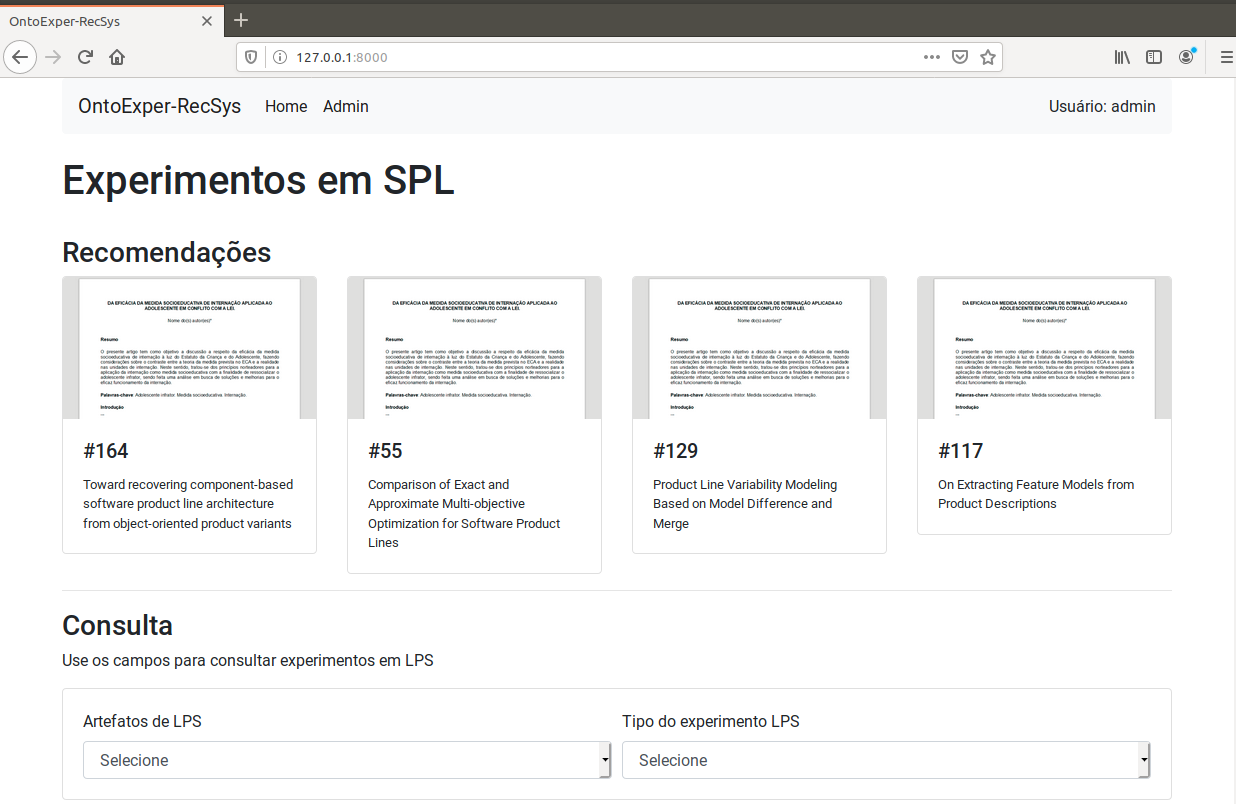
\includegraphics[scale=.35]{tela-recsys-onto.png}
	\caption{Tela do SR.}
	\label{figure:tela-recsys-onto}
\end{figure}

A \ref{figure:tela-recsys-onto} apresenta a tela constru�da para o SR. Nessa tela existem dois campos de consultas, (i) Artefatos de LPS e (ii) Tipo de experimento em LPS. Quando o usu�rio seleciona qualquer um dos dois campos, o SR invoca o m�todo \textit{filter\_experiment()} passando os dados selecionados como par�metro. Nesse m�todo � realizado a infer�ncia na ontologia, segundo os valores que o usu�rio selecionou na tela. A listagem \ref{lst:inferencia-onto} apresenta o c�digo da consulta realizada.

\begin{lstlisting}[language=Python, caption=Infer�ncia na OntoExper-SPL, label=lst:inferencia-onto]
result = onto.search(is_a=onto.Abstract,
	documentation=onto.search(is_a=onto.Documentation,
	  experiment=onto.search(
	    wasTheSPLSourceUsedInformed="*%s*" % sourceSPL,
	    typeExperimentSPL=instance_typeExperimentSPL, 
	    _case_sensitive=False
	    )
	  )
	)
\end{lstlisting}
 

\subsection{Fase 3: \textit{Ratings} dos Usu�rios no SR}

Existem duas formas de gerar avalia��o aos itens em SR, o \textit{rating} expl�cito e o \textit{rating} impl�cito.

\begin{itemize}
	\item No \textit{rating} expl�cito o usu�rio d� uma nota a um item manualmente;
	\item No \textit{rating} impl�cito a nota de um item � inferida a partir do comportamento do usu�rio.
\end{itemize}

Neste projeto de SR foi implementado o modelo de avalia��o expl�cito, onde cada usu�rio d� uma nota a um experimento em LPS. Ap�s o usu�rio realizar um consulta ele pode navegar nos resultados e ao selecionar um experimento na lateral direita � carregado o resumo do mesmo. Nessa lateral foi implementada a op��o do usu�rio dar sua nota. Aqui foi utilizado o modelo estrela, ou seja, o usu�rio tem a op��o de dar de uma a cinco estrelas por experimento. A \ref{figure:rating-recsys-onto} apresenta a tela que com as op��es de \textit{rating} expl�cito.

\begin{figure}[htb]
	\centering 
	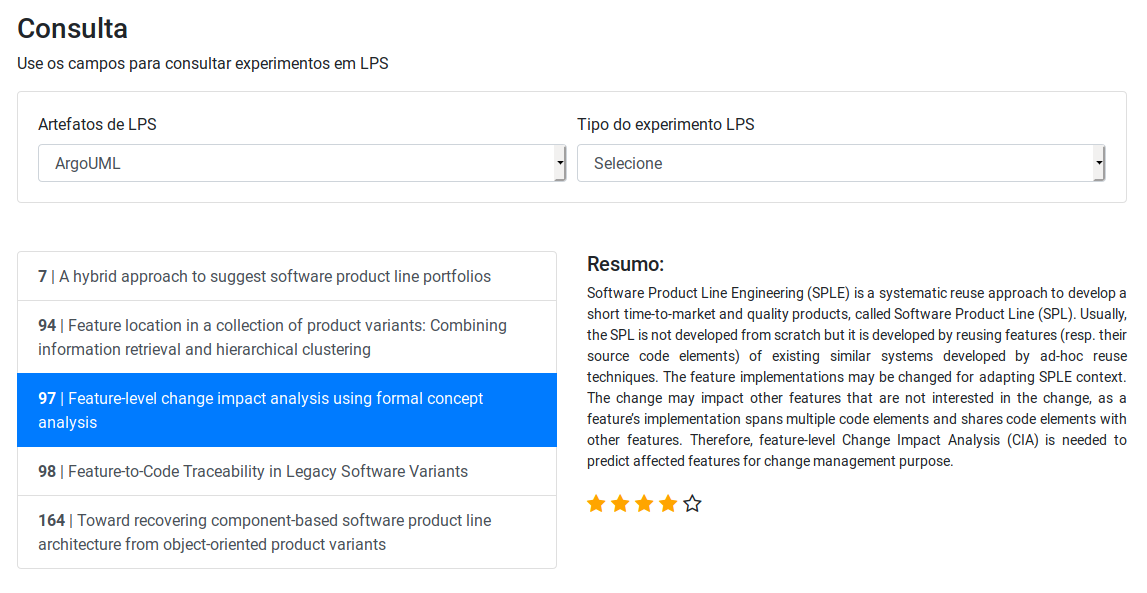
\includegraphics[scale=.5]{rating-recsys-onto.png}
	\caption{\textit{Rating} Expl�cito no SR.}
	\label{figure:rating-recsys-onto}
\end{figure}

Quando o usu�rio d� a sua nota, o SR invoca o m�todo \textit{rating\_experiment()} que recebe como par�metro o experimento e a nota dada pelo usu�rio e realiza a persist�ncia desses dados em um banco de dados relacional, na Se��o \ref{sec:banco_dados} est� detalhada a modelagem desses dados.


\subsection{Fase 4: Modelagem de Recomenda��o, Um Algoritmo para Filtragem Colaborativa}

Neste projeto foi utilizada como abordagem de recomenda��o a filtragem colaborativa. Esse modelo foi implementado utilizando o c�lculo da dist�ncia Euclidiana a fim de encontrar a similaridade entre os usu�rios do SR, em seguida, calcular as poss�veis notas dos itens que o usu�rio em quest�o ainda n�o avaliou e ranquea-las. Dessa forma sendo poss�vel recomendar, sugerindo determinada prioridade, os itens que o usu�rio ainda n�o se relacionou no SR e provavelmente gostaria de interagir.

Para tal resultado o algoritmo est� dividido em tr�s partes: (i) cria��o do \textit{dataset} para o algoritmo, (ii) c�lculo da similaridade - utilizando o c�lculo da dist�ncia Euclidiana e (iii) c�lculo da nota para os itens ainda n�o avaliados.

\begin{itemize}
	\item \textbf{Cria��o do \textit{dataset} para o algoritmo:} esta parte consulta o banco de dados e agrupa as notas dos experimentos por usu�rio, dessa forma gerando uma lista de usu�rio e as notas que ele deu para cada experimento. Por exemplo a lista: ['usu�rio-1': {69: 5.0, 1: 4.0, 5: 1.0, 129: 5.0, 170: 2.0, 97: 4.0}, 'usu�rio-2' {102: 3.0, 117: 4.0, 125: 3.0, 13: 2.0, 9: 3.0, 129: 4.0, 170: 4.0}], pode-se observar que o usu�rio-1 avaliou seis experimentos e o usu�rio-2 sete sendo eles \#102, \#117, \#125, \#13, \#9, \#129 e o \#170 (esses n�meros representam o identificador de cada experimento no SR), cada um com sua respectiva nota. Essa modelagem de dados � necess�ria para os pr�ximos passos do algoritmo.
	
	\item \textbf{C�lculo da similaridade:} a fundamenta��o da dist�ncia Euclidiana � medir a dist�ncia entre dois pontos ou mais, como descrito na Equa��o \ref{eq:distancia_eucliana}. 
	
	\begin{equation}
		\label{eq:distancia_eucliana}
		DE(x,y) = \sqrt{\sum_{i}^{p}{(x_i-y_i)�}}
	\end{equation}
	
	Usou-se este fundamento para encontrar a dist�ncia das notas dadas pelos usu�rios. Por exemplo, dado um determinado experimento com identificador \#170 usu�rio-1 deu nota 2.0 e o usu�rio-2 deu nota 4.0, pelo c�lculo da dist�ncia Euclidiana temos que o usu�rio-1 � distante do usu�rio-2 por um valor 2. Esse c�lculo fica mais interessante quando aplicamos mais dimens�es, cada dimens�o no no nosso cen�rios pode ser associada a um experimento, por exemplo, se for incluido no c�lculo o experimento \#129, tem-se que o usu�rio-1 deu nota 5.0 e o usu�rio-2 deu nota 4.0 logo calculo fica $\sqrt{(2-4)^2+(5-4)^2}$, retornando 3. O pr�ximo passo � normalizar esse valor de retorno da dist�ncia Euclidiana entre 0 e 1, aplicando a Equa��o \ref{eq:normalizacao_de}. Dessa forma pode-se afirmar que neste exemplo a similaridade entre o usu�rio-1 e o usu�rio-2 � 0.25

	\begin{equation}
		\label{eq:normalizacao_de}
		sim = \frac{1}{(1+de)}
	\end{equation}

	Todo algoritmo e c�lculos que foram implementados est�o no arquivo \textit{collaborativeFilter.py} e est� dispon�vel no Ap�ndice \ref{}.

	\item \textbf{C�lculo da nota para os itens ainda n�o avaliados:} esta parte do algoritmo, busca prever uma nota para os itens ainda n�o avaliados pelo usu�rio, para tal efeito � necess�rio realizar um c�lculo de m�dia ponderada usando o c�lculo de similaridade descrito anteriormente, este c�lculo est� descrito na Equa��o \ref{eq:nota_previsao}. Para melhor entendimento do c�lculo, segue o exemplo, dado os experimentos \#129 e \#170, o usu�rio-1 deu nota 2.0 para o \#129 e nota 3.0 para \#170, o usu�rio-2 deu nota 4.0 para o \#129 e nota 5.0 para \#170 e o o usu�rio-3 n�o deu nota para o \#129 e nota 4.0 para \#170, temos um usu�rio-4 queremos encontrar qual nota que ele daria para os experimentos \#129 e \#170, sabendo que o usu�rio-4 tem uma similaridade 0,4 com usu�rio-1, 0,25 com usu�rio-2 e 0,18 com usu�rio-3. a tabela \ref{tab:calculo-ponderado} apresenta os resultados deste c�lculo. Dessa forma podemos dizer que o usu�rio-4 daria nota 3,82 para \#170 e 2,77 \#129, portanto o SR recomendaria o experimento que \#170 por ter maior nota.
	
	\begin{equation}
		\label{eq:nota_previsao}
		NOTA_p() = \frac{\sum_{i}^{usuarios}{(sim_i*nota_i)}}{\sum_{i}^{usuariosTemNota}{(sim_i)}}
	\end{equation}

	\begin{table}[]
		\centering
		\caption{C�lculo para previs�o de nota}
		\label{tab:calculo-ponderado}
		\begin{tabular}{llllll}
		& Sim & Nota \#129 & Sim X \#129 & Nota \#170 & Sim X \#170 \\ \hline
		usu�rio-1 & \textbf{0,40} & \multicolumn{1}{c}{2} & \textbf{0,80} & \multicolumn{1}{c}{3} & 1,20 \\
		usu�rio-2 & \textbf{0,25} & \multicolumn{1}{c}{4} & \textbf{1,00} & \multicolumn{1}{c}{5} & 1,25 \\
		usu�rio-3 & \textbf{0,18} &  & \textbf{0,00} & \multicolumn{1}{c}{4} & 0,72 \\ \hline
		Total &  &  & 1,80 &  & 3,17 \\
		Soma Sim &  &  & 0,65 &  & 0,83 \\
		Total / Soma &  &  & 2,77 &  & 3,82 \\ \hline
		\textbf{usu�rio-4} &  & \textbf{2,77} &  & \textbf{3,82} & 
		\end{tabular}
	\end{table}

\end{itemize}

O modelo de recomenda��o usando foi a filtragem colaborativa com \textit{rating} expl�cito gera o problema da partida fria, ou seja, n�o temos dados o suficientes no SR quando ainda n�o h� avalia��es lan�adas, isso implica em resultados n�o satisfat�rios de recomenda��o. Foi implementado um modelo de nota aleat�ria para resolver este problema. Por�m, a melhor solu��o seria implementar a filtragem baseada em conte�do, pois esse modelo n�o se baseia nos \textit{ratings} dados pelos usu�rios.

\section{Banco de Dados}
\label{sec:banco_dados}

Para o banco de dado do SR foi utilizado o SGBD SQLite\footnote{https://www.sqlite.org/index.html}, ele foi utilizado por ser o banco de dados padr�o para Django Framework, dessa forma n�o foi preciso realizar nenhuma outra configura��o. O SQLite � um dos bancos de dados mais simples, todos os registros de metadados s�o armazenados em um �nico arquivo. 

As entidades existentes no banco de dados, s�o:

\begin{itemize}
	\item auth\_group;
	\item auth\_group\_permissions;
	\item auth\_permission;
	\item auth\_user;
	\item auth\_user\_groups;
	\item auth\_user\_user\_permissions;
	\item django\_admin\_log;
	\item django\_content\_type;
	\item django\_migrations;
	\item django\_session;
	\item rating\_rating; e
	\item sqlite\_sequence.
\end{itemize}

As entidades com prefixo \textit{auth} e \textit{django} s�o geradas e mantidas pelo pr�prio Django Framework. A entidade \textit{rating\_rating} foi gerada pela aplica��o \textit{rating} dentro do projeto, a \ref{tab:tabela-rating} descreve sua estrutura. Sua fun��o � armazenar as avalia��es dos usu�rio, a coluna \textit{user} armazena o login do usu�rio, a coluna rating armazena a nota dada, a coluna id\_experiment armazena o id do experimento e a coluna title\_experiment armazena o t�tulo do experimento.

\begin{table}[]
	\centering
	\caption{Entidade \textit{rating\_rating} do Banco de Dados}
	\label{tab:tabela-rating}
	\begin{tabular}{@{}ll@{}}
	\toprule
	Propriedade & Tipo \\ \midrule
	id & integer \\
	user & varchar(50) \\
	rating & real \\
	id\_experiment & integer \\
	title\_experiment & varchar(255) \\ \bottomrule
	\end{tabular}
\end{table}


\section{Ambiente de Desenvolvimento}
\label{sec:ambiente_de_desenvolvimento}

Para o desenvimento do SR foram necess�rias algumas ferramentas de apoio, al�m do Django Framework e do SQLite j� citado, foram utilizadas outras tecnologias como HTML CSS e JS, com o apoio dos \textit{frameworks} Bootstrap\footnote{https://getbootstrap.com/} e jQuery\footnote{https://jquery.com/}.

Para ambiente de desenvolvimento de c�digo fonte foi utilizado o editor de texto VSCode\footnote{https://code.visualstudio.com/} da Microsoft e a ferramenta Jupyter-Notebook e Jupyter-Lab, para visualiza��o do SR o navegador Google Chrome e FireFox e para o banco de dados o DB Browser\footnote{https://sqlitebrowser.org/}. Todas essas ferramentas s�o \textit{open source} e est�o disponiveis para \textit{download} at� a data de escrita deste trabalho.

Foram escolhidas essas ferramentas, pois o pesquisador j� possu�a habilidades nelas e por possuir maturidade e reconhecimento na ind�stria de desenvolvimento de software.

%TODO
\section{Empacotamento e Compartilhamento}
\label{sec:recsys_empacotamento}

Os artefatos utilizado para o desenvolvimento do SR est�o dispon�veis em: https://doi.org/..., visando dissemina��o dos dados.


\section{Considera��es Finais}
\label{sec:recsys_consideracoes_finais}

Este cap�tulo apresentou um SR provando que � poss�vel realizar infer�ncias no modelo de ontologia proposto por este trabalho de mestrado, a OntoExper-SPL. Por meio das infer�ncias implementadas no SR, foi poss�vel implementar o modelo de recomenda��o \textit{collaborative filtering} e gerar recomenda��es para os usu�rios que interagirem com o SR.

Inicialmente, a termo de contexto, foi apresentados os conceitos b�sico de sistemas de recomenda��o e uma breve descri��o do modelo \textit{collaborative filtering}. Na sequ�ncia foi apresentado como os sistemas de recomenda��o s�o tratados na ES e alguns exemplos de aplica��o.

Foi apresentado na se��o de concep��o do SR, a modelagem inicial da aplica��o, as principais tecnologias abordadas antes da fase de implementa��o, o ecossistema Python serviu como base para o desenvolvimen geral do SR, desde a infer�ncias iniciais at� a implementa��o de modelo de recomenda��o. J� na se��o de projeto foi tratado especificamente de como as tecnologias e ferramentas auxiliaram em cada fase do projeto, que foram divididas em quatro fases, (i) cria��o do projeto de aplica��o web usando Django Framework, (ii) carregamento da OntoExper-SPL no SR, (iii) \textit{ratings} dos usu�rios no SR e (iv) implementa��o do modelo de recomenda��o. O Django Framework se destaca pois ele foi a base de implementa��o da aplica��o web, pois ele foi constru�do para esse prop�sito, implementando principalmente os conceitos de MVC. Posteriormente foi apresenta o banco de dados e sua principal tabela para SR, a tabela que armazena os \textit{ratings} do usu�rio. Por fim, foi apresentado o ambiente de desenvolvimento utilizado para elaborar do SR, a principal ferramente para este fim foi o editor de texto VSCode.

No pr�ximo cap�tulo, ser� apresentado a conclus�o final deste trabalho de mestrado.


% \chapter{Proposta de Melhorias e Trabalhos Futuros para SMartOntology}
\pagestyle{plain}
\label{sec:melhorias_trabalhos_futuros}

Este t�pico apresenta propostas de melhorias e trabalhos futuros a serem aplicadas a SMartOntology.

\section{Considera��es Iniciais}
\label{sec:concidaracoes_iniciais}


\section{Propostas de Melhoria da Avalia��o}
\label{sec:propostas_de_melhoria}


\section{Trabalhos Futuros}
\label{sec:trabalhos_futuros}


\section{Considera��es Finais}
\label{sec:concidaracoes_finais}
\chapter{Conclus�o}
\pagestyle{plain}
\label{sec:conclusao}


\section{Considera��es Iniciais}
\label{sec:concidaracoes_iniciais}

...

A realiza��o de experimentos de SE no SPL traz informa��es mais relevantes para fornecer evid�ncias de uma teoria para o mundo real. A capacidade de entender, estudar e replicar experimentos torna esse m�todo ainda mais rico. Ao organizar os dados e informa��es sobre os experimentos de SE no SPL, acreditamos que essa tarefa � mais f�cil. Usando as tecnologias adjacentes, tais como formalizar o conhecimento atrav�s de ontologias e infer�ncias para gerar dados de informa��o personalizada atrav�s de um sistema de recomenda��o.

Neste trabalho, foi desenvolvida uma proposta para um modelo de ontologia (SMartyOntology) com o objetivo de organizar e estruturar o conhecimento adquirido sobre experimentos de SE em SPL. Este conhecimento foi previamente levantado em um trabalho de disserta��o do nosso grupo de pesquisa, onde foram relatados mais de 200 artigos que relatam experimentos em SPL. Com este levantamento foi poss�vel criar um modelo de ontologia para representar o conhecimento sobre experimentos em NPS, inserindo os dados dos artigos neste modelo, denominamos esta fase de inser��o dos indiv�duos na ontologia. Desta forma, estruturamos o TBox e o Abox para a SMartyOntology. Com a composi��o da ontologia podemos fazer uma breve avalia��o sobre algumas armadilhas que o modelo de ontologia poderia ter, utilizamos a ferramenta OOPS! para esta avalia��o. Tamb�m foi poss�vel criar um exemplo simples de recomenda��o, fazendo a infer�ncia das informa��es para a SMartyOntology.

A SMartyOntology se destaca por levar em conta um dom�nio espec�fico de experimentos de SE. SPL s�o constru�dos atrav�s de um dom�nio de aplica��o, semelhan�as, avalia��es do n�cleo e variabilidades, que distingue um produto do outro dentro da fam�lia de produtos, todas essas caracter�sticas est�o presentes na ontologia. No entanto, a SMartyOntology pode ser facilmente estendida a outros dom�nios de experimentos de SE, uma vez que todas as classes dentro da ontologia que lidam com SPL s�o subclasses de representa��es de experimentos em geral.

Os principais objetivos deste trabalho, est�o relacionados a propor um sistema de recomenda��o que, possa gerar processos e diretrizes para realiza��o de experimentos em LPS. Para foi realizado um estudo aprofundado nos conceitos de Sistemas de Recomenda��o em ES e modelos de Ontologias para representa��o dos dados levantados sobre a qualidade dos experimentos em LPS, encontrados no trabalho do grupo.

Portanto, acredita-se que ap�s a realiza��o do projeto de software, ser� poss�vel desenvolver o sistema de recomenda��o para que os usu�rios que interagirem com este sistema, e possa receber recomenda��es de processos e diretrizes para suas pesquisas experimentais em LPS.

Como trabalho futuro, identificamos na avalia��o v�rios pontos de melhoria na modelagem da ontologia, esses ajustes devem ser feitos para padronizar o modelo com o objetivo de possibilitar a extens�o e divulga��o do mesmo.


\section{Considera��es Finais}
\label{sec:concidaracoes_finais}

... 

% Fancyhead
\fancyhead[RO,LE]{\itshape REFER�NCIAS}
\fancyhead[RO,LE]{\thepage}

% Bibliografia

\renewcommand{\bibname}{REFER�NCIAS} 
%\setlength\bibindent{0mm}
\setlength\bibhang{0mm} 
%\bibliographystyle{apalike}
\bibliographystyle{icmc2}
\bibliography{texto/RevisaoLiteratura}

% Ap�ndices
\initappendix

\appendix{Apêndice A: Código Fonte do Modelo da SMartOntology}
\label{apendice:a}
\appendix{Ap�ndice B: C�digo Fonte do Povoamento de Dados no Modelo OntoExper-SPL}
\label{apendice:b}
\appendix{Ap�ndice B: C�digo Fonte do Povoamento de Dados no Modelo OntoExper-SPL}
\label{apendice:b}
\appendix{Ap�ndice D: C�digo Fonte dos Exemplos de Aplica��o de Recomenda��o Usando SMartOntology }
\label{apendice:d}

\end{document}
